\documentclass[a4paper]{article}
\usepackage[utf8]{inputenc}
\usepackage[T1]{fontenc}

\usepackage[backend=biber,sorting=none]{biblatex}
\addbibresource{references.bib}

\usepackage{amsmath}
\usepackage{appendix}
\usepackage{graphicx}
\usepackage{hyperref}
\usepackage{listings}
\usepackage{placeins}
\usepackage{subcaption}
\usepackage{tabularx}
\usepackage{xcolor}

% \DeclareUnicodeCharacter{03BC}{\textmu}
% \DeclareUnicodeCharacter{B5}{\textmu}

% For fixing unicode errors with lstinputlisting
% https://en.wikibooks.org/wiki/LaTeX/Source_Code_Listings#Encoding_issue
\lstset{literate=
	{µ}{{\textmu}}1
}

\title{PAP328 project work: proportional counter}
\author{Mika Mäki}
\date{2021-04-10}
% TODO add date when the report was handed in

\newenvironment{todo}{
% \hline
\color{red}
}
{
% \hline
}


\begin{document}

\maketitle

\section*{Abstract}
In this project we assembled a gas-based proportional counter for X-ray and $\gamma$-ray detection.
The detector consists of a drink can that serves as the cathode, and a thin anode wire along its center.

% When high voltage is applied between the cathode and the anode and incoming high-energy radiation ionizes the gas inside, the resulting electrons drift towards the anode wire.
% Close to the wire the field strength is high enough for avalanche formation, and the electrons are multiplied, resulting in an electrical pulse that can be detected with read-out electronics.

The system was tested with Fe-55 and Am-241 sources, and a multichannel analyzer was used to collect the emission spectra, which were then analyzed with self-developed software.
This setup demonstrated sufficient resolution to distinguish the TODO peaks.

% TODO add main results here.

The detector was also tested with a self-built pre-amplifier.
However, these results were inconclusive due to unexpected degradation of the detector.

\tableofcontents


\section{Introduction}
\label{introduction}
Radiation detectors are devices that measure the rate of incoming ionizing radiation such as $\alpha$, $\beta$, $\gamma$ and neutrino radiation and optionally measure its kinetic energies.
They are widely used on various fields from nuclear energy production to medicine.
The properties of ionizing radiation and the needs of applications vary, and so do the detector principles and constructions used.

However, a common feature of particle detectors has been that they are expensive and require various specific tools and materials to manufacture.
In this project work we followed in the footsteps of
\href{https://www.helsinki.fi/en/people/people-finder/alexander-winkler-9110087}{Winkler}
et al. \cite{winkler_gaseous_2015} to demonstrate that proportional counters can be an exception to this by manufacturing a relatively simple proportional counter based on a conventional drink can.
Proportional counters are gas-based radiation detectors, which as their name suggests, produce electric pulses with amplitudes proportional to the energies of the incoming ionizing radiation.
Their operation principles are discussed in section \ref{theory}.

The construction of the proportional counter is discussed in section \ref{assembly}.
To obtain accurate and meaningful results, the system had to be calibrated as in section \ref{assembly} and configured for the measurements as in section \ref{setup_testing}.
The results for the calibration, high voltage sweep and spectral measurements are discussed in section \ref{results}.

We also constructed our own pre-amplifier, but the results were inconclusive due to unexpected degradation of the detector.
These measurements are discussed in the appendix \ref{pre_amp}.


\section{Theory}
\label{theory}

\subsection{Radiation sources and interaction of their radiation with matter}
Radiation can be categorized to ionizing and non-ionizing radiation depending on its capability of exciting electrons out of matter.
In the context of particle physics, the most relevant type of radiation is ionizing radiation, which includes particle radiation and short-wavelength electromagnetic radiation such as X-rays and gamma radiation.
Non-ionizing radiation refers primarily to electromagnetic radiation of visible and longer wavelengths.
In addition to these there are other forms of radiation such as neutrons and neutrinos.

The effects of electromagnetic radiation vary significantly by wavelength.
Whereas the longer wavelengths are mostly capable of inducing thermal motion, other excitations and electric currents, the shorter wavelengths from ultraviolet radiation onwards have enough energy to remove an electron from an atom or a molecule and are therefore ionizing.

Radiation can be characterized
\cite{knoll_radiation_2010}

However, the details of the interaction of high-energy photons with matter vary significantly by wavelength.

Alpha and beta radiation are the most prominent types of particle radiation.
Alpha radiation consists of 

In this project work we used $^{55}$Fe and $^{241}$Am sources.
Both emit various types of radiation in their decay processes, but due to their closed packaging, only electromagnetic radiation was allowed to escape the sources.
$^{55}$Fe decays by electron capture of the innermost shell (K-shell) into $^{55}$Mn with a half-life of 2.75 a.
This results in an electron vacancy, which gets filled by an electron from the outer shells, resulting in a sequence of electron transfers, the energy of which is released as Auger electrons and X-ray emissions.


\begin{equation}
^{241}_{95}\text{Am} \rightarrow ^{237}_{93}\text{Np} + ^4_2 \alpha + \gamma (59.24 \text{keV})
\end{equation}



In this project we used an

In this project we focus on x-rays and alpha, beta and gamma radiation.




\subsection{The proportional counter}
\label{counter}

In this project the particle detection was done using a proportional counter, which is a gas-filled particle detector with a high electric field inside.
\cite{instructions}
A schematic of the proportional counter is given in figure \ref{fig:theory_schematic}.

\begin{figure}[ht!]
\centering
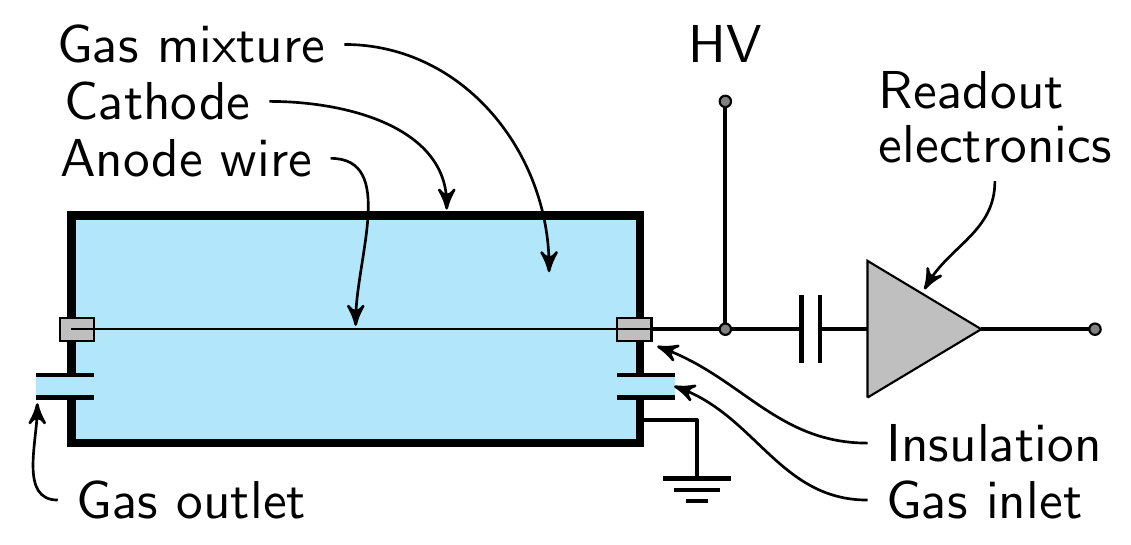
\includegraphics[width=0.6\textwidth]{fig/article/schematic.png}
\caption{Schematic drawing of the proportional counter \cite{winkler_gaseous_2015}}
% TODO: draw own version with vector graphics
\label{fig:theory_schematic}
\end{figure}

When ionizing radiation passes through the detector, it collides with the gas inside, causing ionization of the gas.
Due to the electric field the electrons drift towards the anode, and the positive ions drift towards the cathode.
This causes a pulse of electric current, which is detectable with the readout electronics.
The detector is cylindrically symmetric, and the electric field strength can therefore be approximated as
\begin{equation}
E(r) = \frac{U}{r \ln(b/a) },
\end{equation}
where $U$ is the potential between the electrodes, $r$ is the radius of the can, $a$ is the outer radius of the anode wire and $b$ is the inner radius of the cathode tube.
Consequently, the electric field strength increases when approaching the anode wire, and close to the anode ($\approx$ 30 \textmu m) it reaches sufficient level for
\href{https://en.wikipedia.org/wiki/Townsend_discharge}{Townsend avalanche} formation.
In a Townsend avalanche the kinetic energy of a drifting electron is sufficient to ionize the gas upon collisions, and this results in the multiplication of the incomng electron.
As the naming of the proportional counter suggests, the number of generated electron-ion pairs is proportional to those generated by the incident radiation, and consequently incoming particles of different energies can be distinquished to create spectral measurements.
\cites{winkler_gaseous_2015}[p. 159--164]{knoll_radiation_2010}

The uniformity of the detector and especially the anode wire is highly important for the spectral accuracy of the detector.
However, in the ends of the detector this is not achieved, as the field distortion caused by the shape of the detector is significant.
As a solution the anode wire at the ends is covered by metallic field tubes, which increase the radius of the anode and consequently prevent the formation of avalanches in those regions.
\cite[p. 165]{knoll_radiation_2010}

Each avalanche creates a cloud of positive ions near the anode, and these slowly diffuse towards the cathode.
The anode wire is long compared to the avalanche, and therefore the detector can record other pulses from other regions of the wire before the ions have cleared from the first one.
However, the applied voltage and consequently the electric field is too high, the avalanches become so large that the ions form a significant space charge in the detector, which alters its characteristics and causes nonlinearities in its behaviour.
This is known as the limited proportionality region.
If the applied voltage is increased further, the space charge becomes a dominant feature.
It reduces the field near the anode and therefore limits the avalanche process, causing all pulses to have the same amplitude.
This is known as the Geiger-Mueller region.
\cite[p. 160--161]{knoll_radiation_2010}

The choice of the gas mixture is essential for the operation of the detector.
The operation of a proportional counter is dependent on the migration of free electrons, which should not be absorbed during their journey.
The gas should therefore have a low electron attachment coefficient.
This disqualifies the use of air, and the detectors should consequently be airtight to prevent the introduction of air into the detector chamber.
\cite[p. 167--168]{knoll_radiation_2010}

The avalanche collisions near the anode wire may cause excitations of the gas in addition to the desired ionization.
These excitations decay by the emission of visible or UV photons, which can cause ionization elsewhere in the detector under suitable circumstances.
These would lead to a loss of proportionality or the creation of spurious pulses, which are undesirable in proportional counters.
To alleviate this problem, a molecular gas is introduced into the mixture to absorb these photons.
In this project we used the P-10 gas mixture, which consists of 90 \% argon and 10 \% methane.
\cite[p. 168]{knoll_radiation_2010}


Gas constants \cite{wolff_measurement_1974}

Theoretical predictions on accuracy?

Schockley \cite{shockley_currents_1938}
Ramo \cite{ramo_currents_1939}
TODO

Diethorn formula \cite[eq. 6.10]{knoll_radiation_2010}
\begin{equation}
\ln M = \frac{V}{\ln b/a} \frac{\ln 2}{\Delta V}
\left( \ln \frac{V}{pa \ln (b/a)} - \ln K \right)
\end{equation}


\subsection{Error analysis methods}
\label{error_analysis}
The detector consists of various components, each of which has its manufacturing imperfections.
In addition, each of the measurement systems used has inaccuracies.
Together these provide various sources of uncertainties for the measurements, and combining these into uncertainties of the end results is known as error propagation.

By Taylor expanding the function in question around the mean values of the random variables we can relate the covariance matrices and therefore the uncertainties of the input and output variables.
In the general case the covariance matrix of the output variables is given by
\begin{equation}
U_{kl}
= \mathrm{Cov}(y_k, y_l)
\approx \sum_{i,j=1}^n \left( \frac{\partial y_k}{\partial x_i} \frac{\partial y_l}{\partial x_j} \right)_{\mathbf{x}=\mathbf{\mu}} V_{ij},
\end{equation}
where $U$ is the covariance matrix of the output variables $y$ and $V$ is the covariance matrix of the input variables $x$.
Consequently the variances for each of the output variables are
\begin{equation}
\sigma_{y_k}^2 \approx \sum_{i,j=1}^n \left( \frac{\partial y_k}{\partial x_i} \frac{\partial y_k}{\partial x_j} \right)_{\mathbf{x}=\mathbf{\mu}} V_{ij}.
\end{equation}
This can be written in matrix notation as
\begin{equation}
U = AVA^T,
\end{equation}
where
\begin{equation}
A_{ij} = \frac{\partial y_i}{\partial x_j} \vert_{\boldsymbol{x}=\boldsymbol{\mu}}.
\end{equation}
\cite[p. 20--22]{cowan_statistical_1998}

If the input variables $x_i$ are uncorrelated, these expressions are simplified.
Then the covariance matrix is given by
\begin{equation}
U_{kl} \approx \sum_{i=1}^n \left( \frac{\partial y_k}{\partial x_i} \frac{\partial y_l}{\partial x_i} \right)_{\mathbf{x}=\mathbf{\mu}} \sigma_i^2,
\end{equation}
and the variances are \cite[p. 20--22]{cowan_statistical_1998}
\begin{equation}
\sigma_{y_k}^2 \approx \sum_{i=1}^n \left( \frac{\partial y_k}{\partial x_i} \right)_{\mathbf{x}=\mathbf{\mu}}^2 \sigma_i^2.
\label{eq:variance}
\end{equation}
In the analysis code of this project the general case of this error propagation has been implemented symbolically using
\href{https://www.sympy.org/}{SymPy}
for use with the computation of the collected charges and the Diethorn formula.
The error propagation of fit functions is handled directly by the
\href{https://docs.scipy.org/doc/scipy/reference/generated/scipy.optimize.curve_fit.html}{scipy.optimize.curve\_fit}
and
\href{https://docs.scipy.org/doc/scipy/reference/generated/scipy.odr.ODR.html}{scipy.odr.ODR} utilities of
\href{https://www.scipy.org/}{SciPy}
that are used to generate the fits.
\cite{repo}


\iffalse
\subsection{Error analysis}
\begin{todo}
The total gain of the amplifiers is a product of the gains of the pre-amplifier and the spectral amplifier.
Therefore the uncertainty of the gain using equation \ref{eq:variance} is
\begin{equation}
\sigma_g \approx \sqrt{(g_\text{spec} \sigma_\text{pre})^2 + (g_\text{pre}\sigma_\text{spec})^2}.
\end{equation}
TODO: the gain of the spectral amplifier was varied from $10\cdot1=10$ to $10\cdot100=1000$, but what was the gain of the pre-amplifier?
Since they were two parts of the same device, was the setting already a total of these?
Was the coarse gain perhaps for the pre-amplifier and the fine gain for the spectral amplifier?
\end{todo}
\fi


\subsection{Read-out electronics}
\label{electronics}


Capacitive decoupling \ref{fig:theory_schematic}

The detector was also tested with a custom pre-amplifier, and the results are in appendix \ref{pre_amp}.


\clearpage
\section{Experimental set-up}
\label{setup}
As a part of this project we built the detector ourselves from a construction kit designed by the course organizers.
For the read-out electronics we used devices available in the laboratory.

Answer the questions on page 5 of the instructions!


\subsection{Detector assembly}
\label{assembly}
We manufactured the detector of this project from an aluminum drink can according to the schematic of figure \ref{fig:schematic}.
The parts were provided by the course organizers, except for the drink can.

\begin{figure}[ht!]
\centering
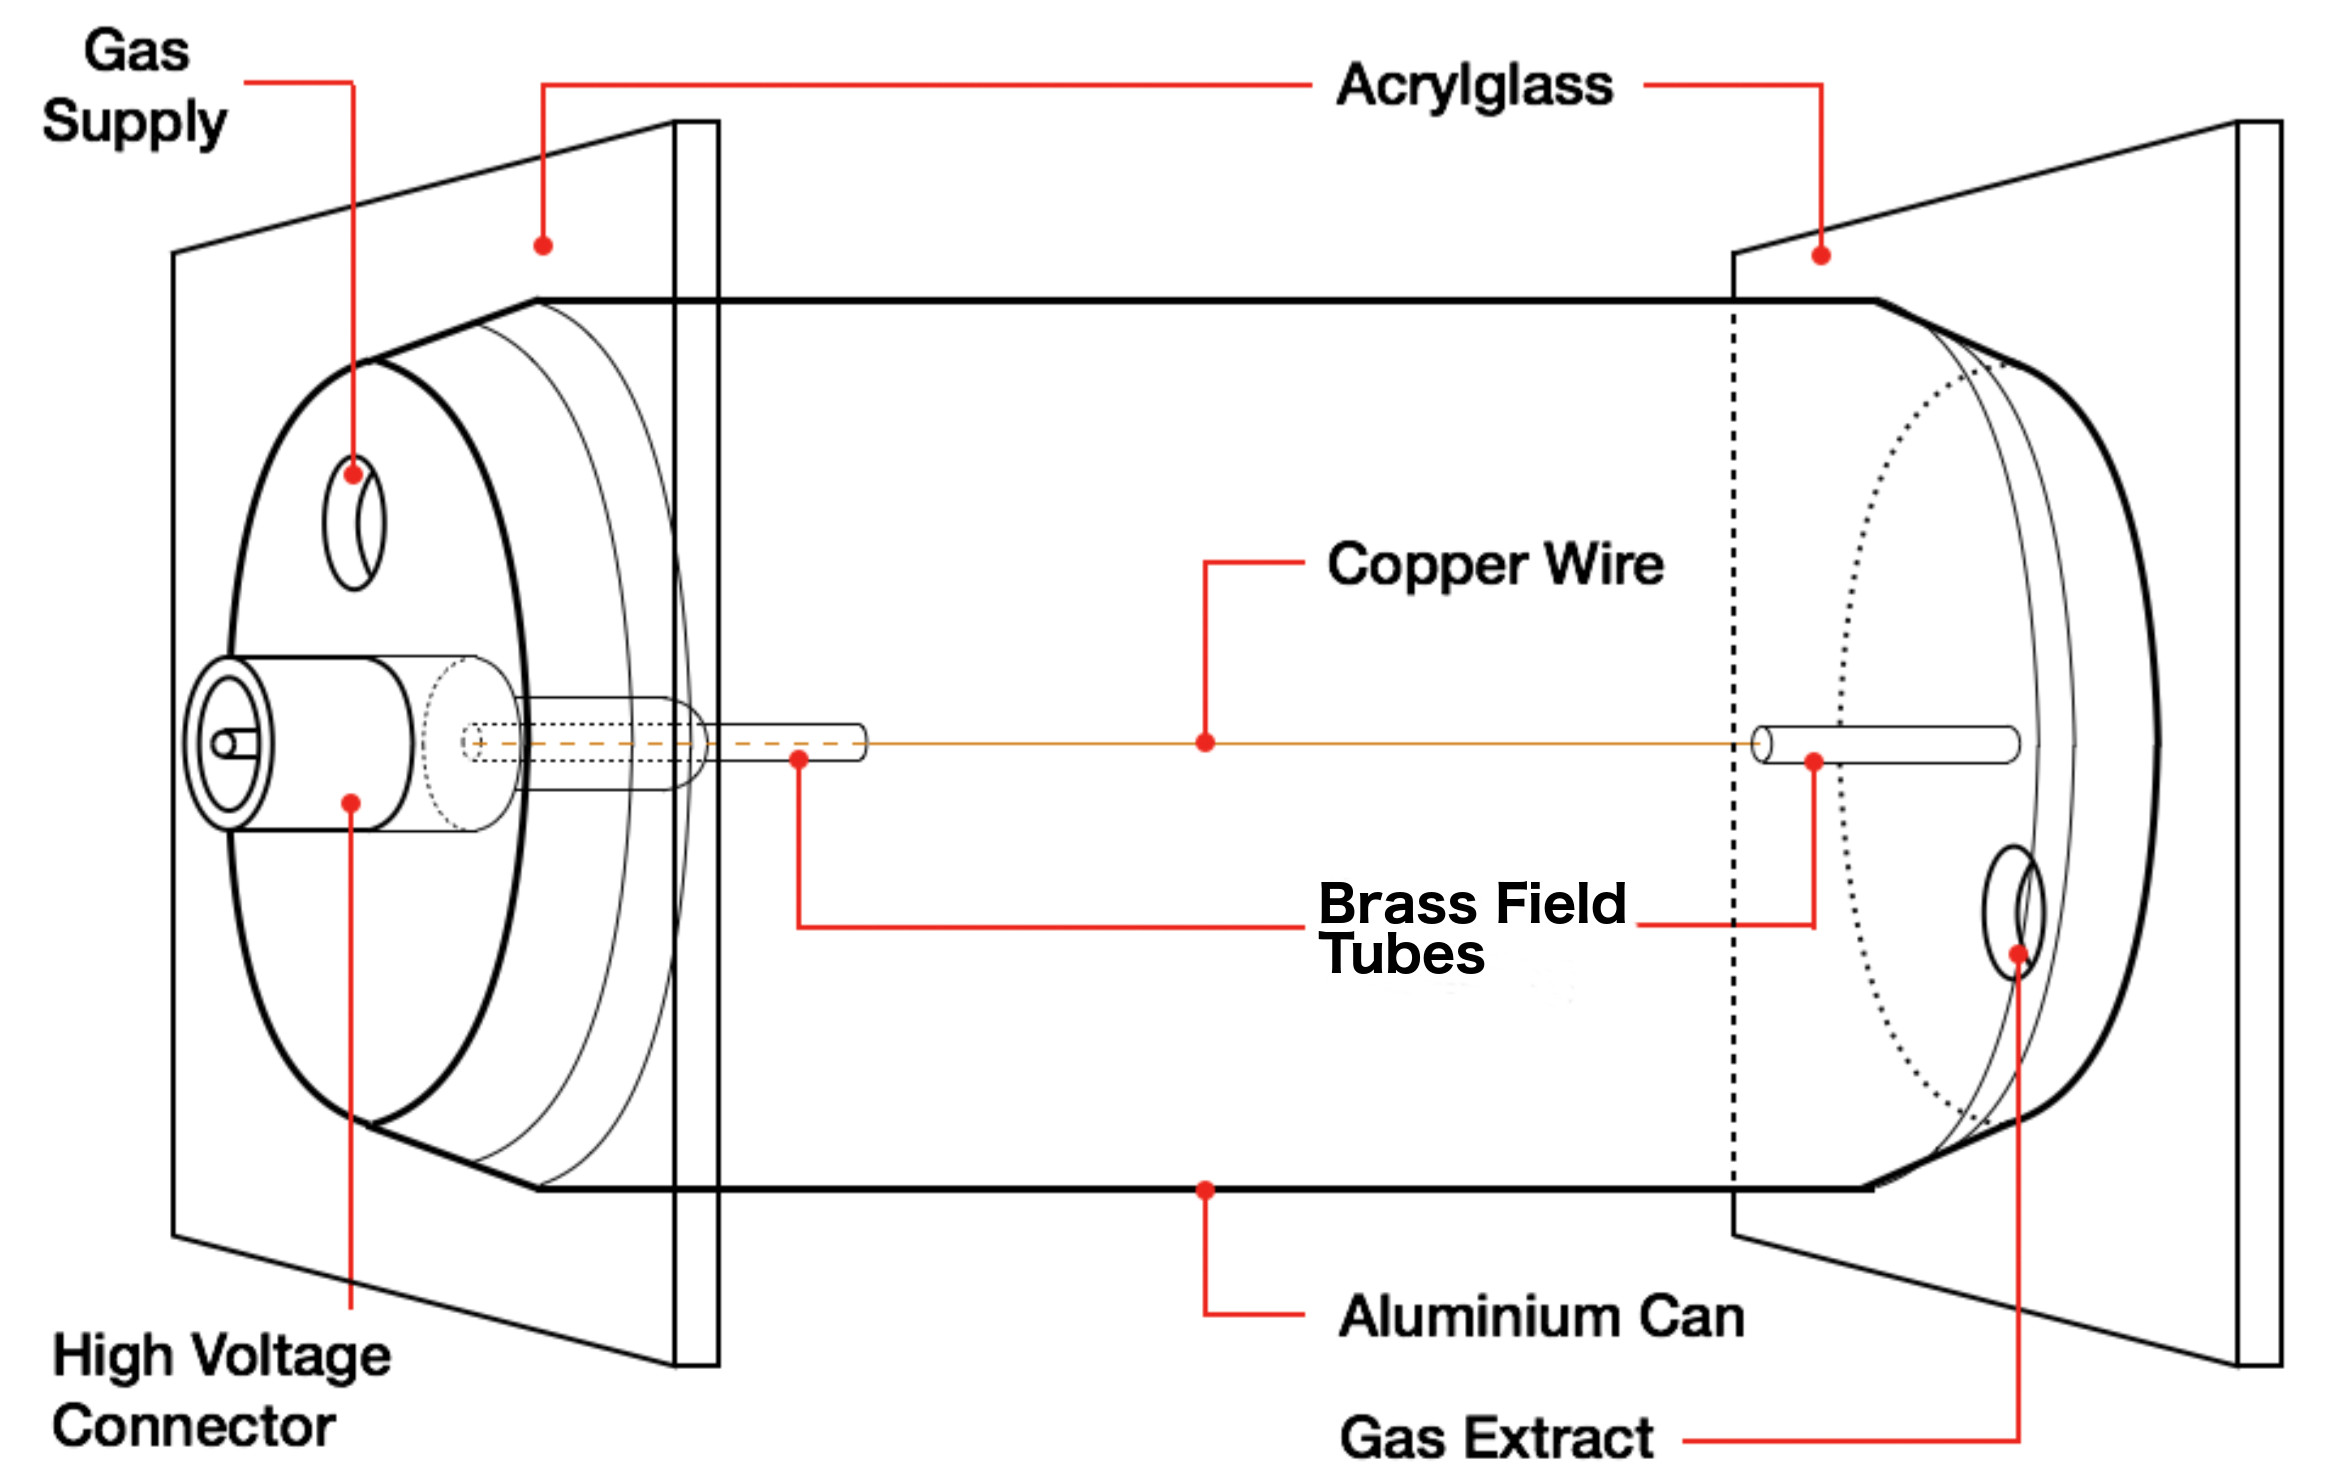
\includegraphics[width=0.8\textwidth]{fig/instructions/schematic.png}
\caption{Schematic of the detector \cite{instructions}}
% TODO draw own one with vector graphics
\label{fig:schematic}
\end{figure}

First we prepared the parts of the detector by removing a single strand from a copper wire and cutting two pieces of brass tube for the wire mounting.
The course organizers removed the top of the can and drilled two holes to its bottom, one to the center and one off-center.
We then smoothened the cutting edges to avoid sharp edges that could cause sparking, and grinded away the anti-corrosion layer for long-term stability of the detector.
Table \ref{table:sizes} contains size measurements of the can and the brass tubes.
Each of the results is averaged from five measurements.
The can thickness and brass tube diameter were measured using a
\href{https://en.wikipedia.org/wiki/Micrometer}{micrometer}, and the rest were measured with a
\href{https://en.wikipedia.org/wiki/Calipers}{caliper}.

Once the can and the other parts were ready, we put them to an ultrasonic cleaner for grease removal, as any leftover grease in the detector could interact due to the high-voltage conditions, causing degradation of detector performance.
To avoid contaminating the cleaned parts, every step from now on had to performed with rubber gloves.

We prepared the anode mounting by gluing the longer brass tube 
to the hole in the center of a plastic screw.
To avoid filling the hole within the brass tube, the outside of the brass tube was coated with glue, and the tube was then pushed into the hole.
The screw was then attached to the can with a plastic nut, as in figure \ref{fig:anode_mounting}.

\begin{figure}[ht!]
\centering
\begin{subfigure}[t]{0.48\textwidth}
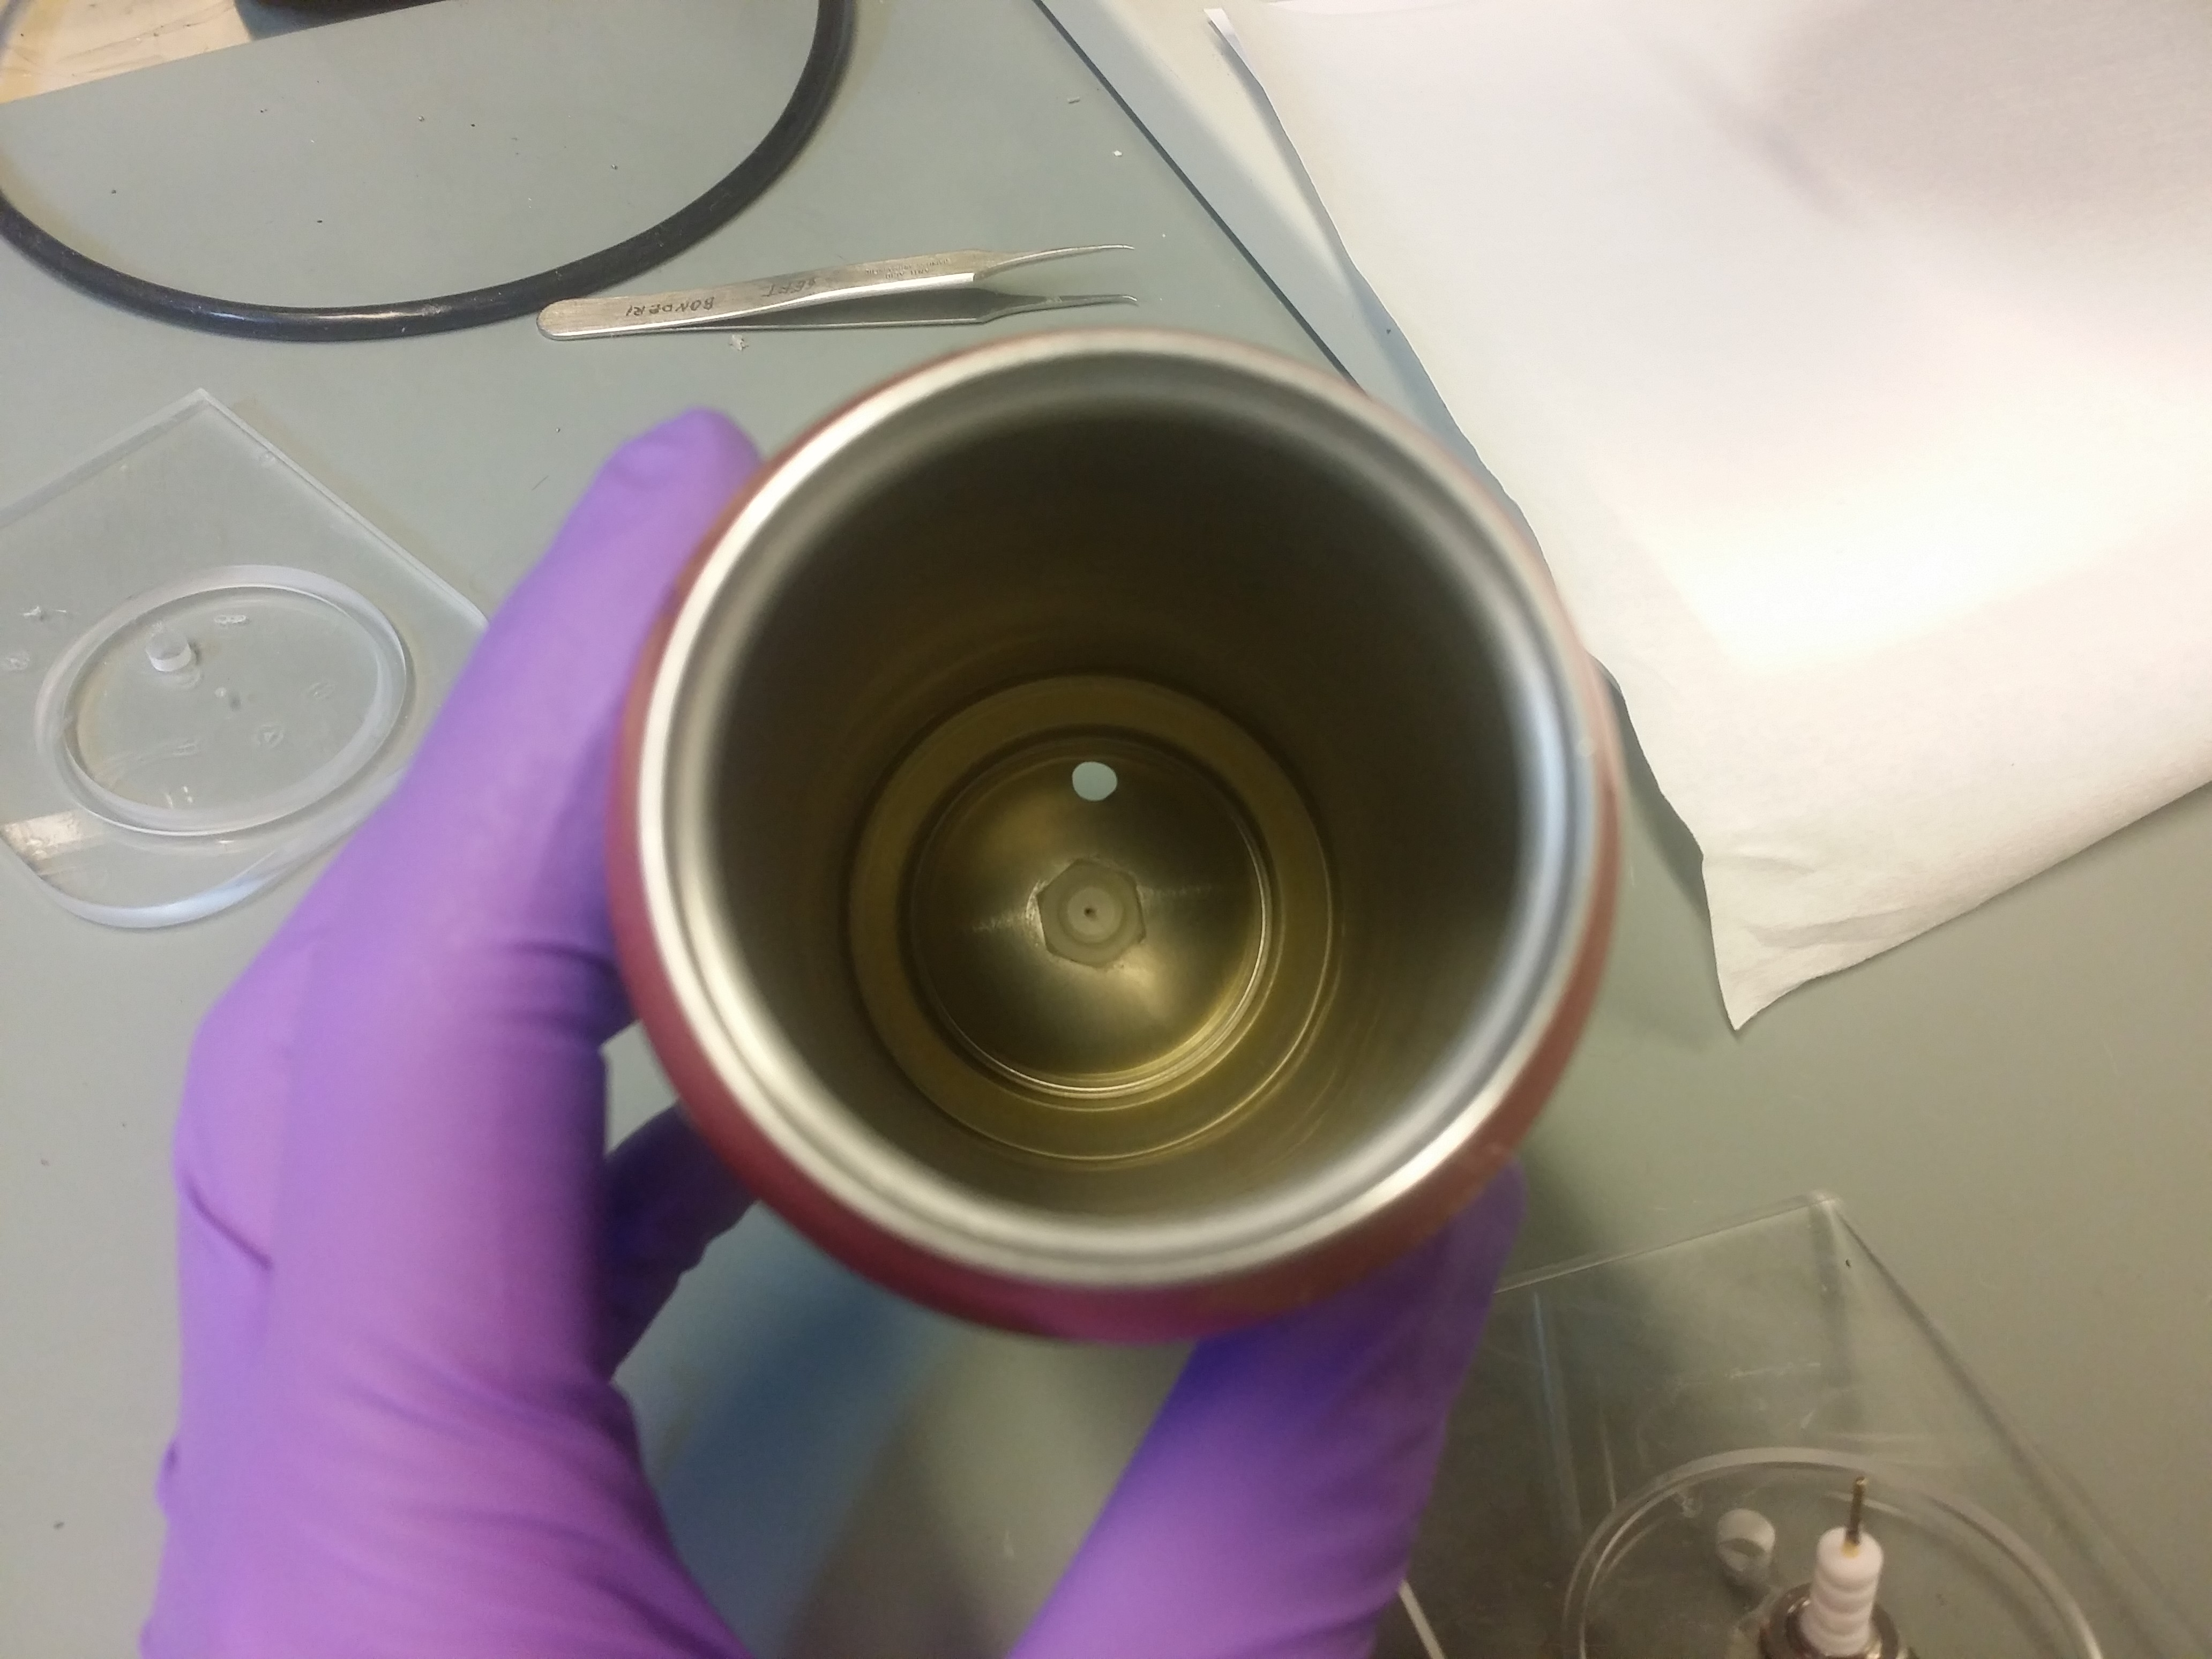
\includegraphics[width=\textwidth]{fig/IMG_20201123_103327.jpg}
\caption{A brass tube within a plastic screw serves as the other end of the anode wire}
\label{fig:anode_mounting}
\end{subfigure}
%
\begin{subfigure}[t]{0.48\textwidth}
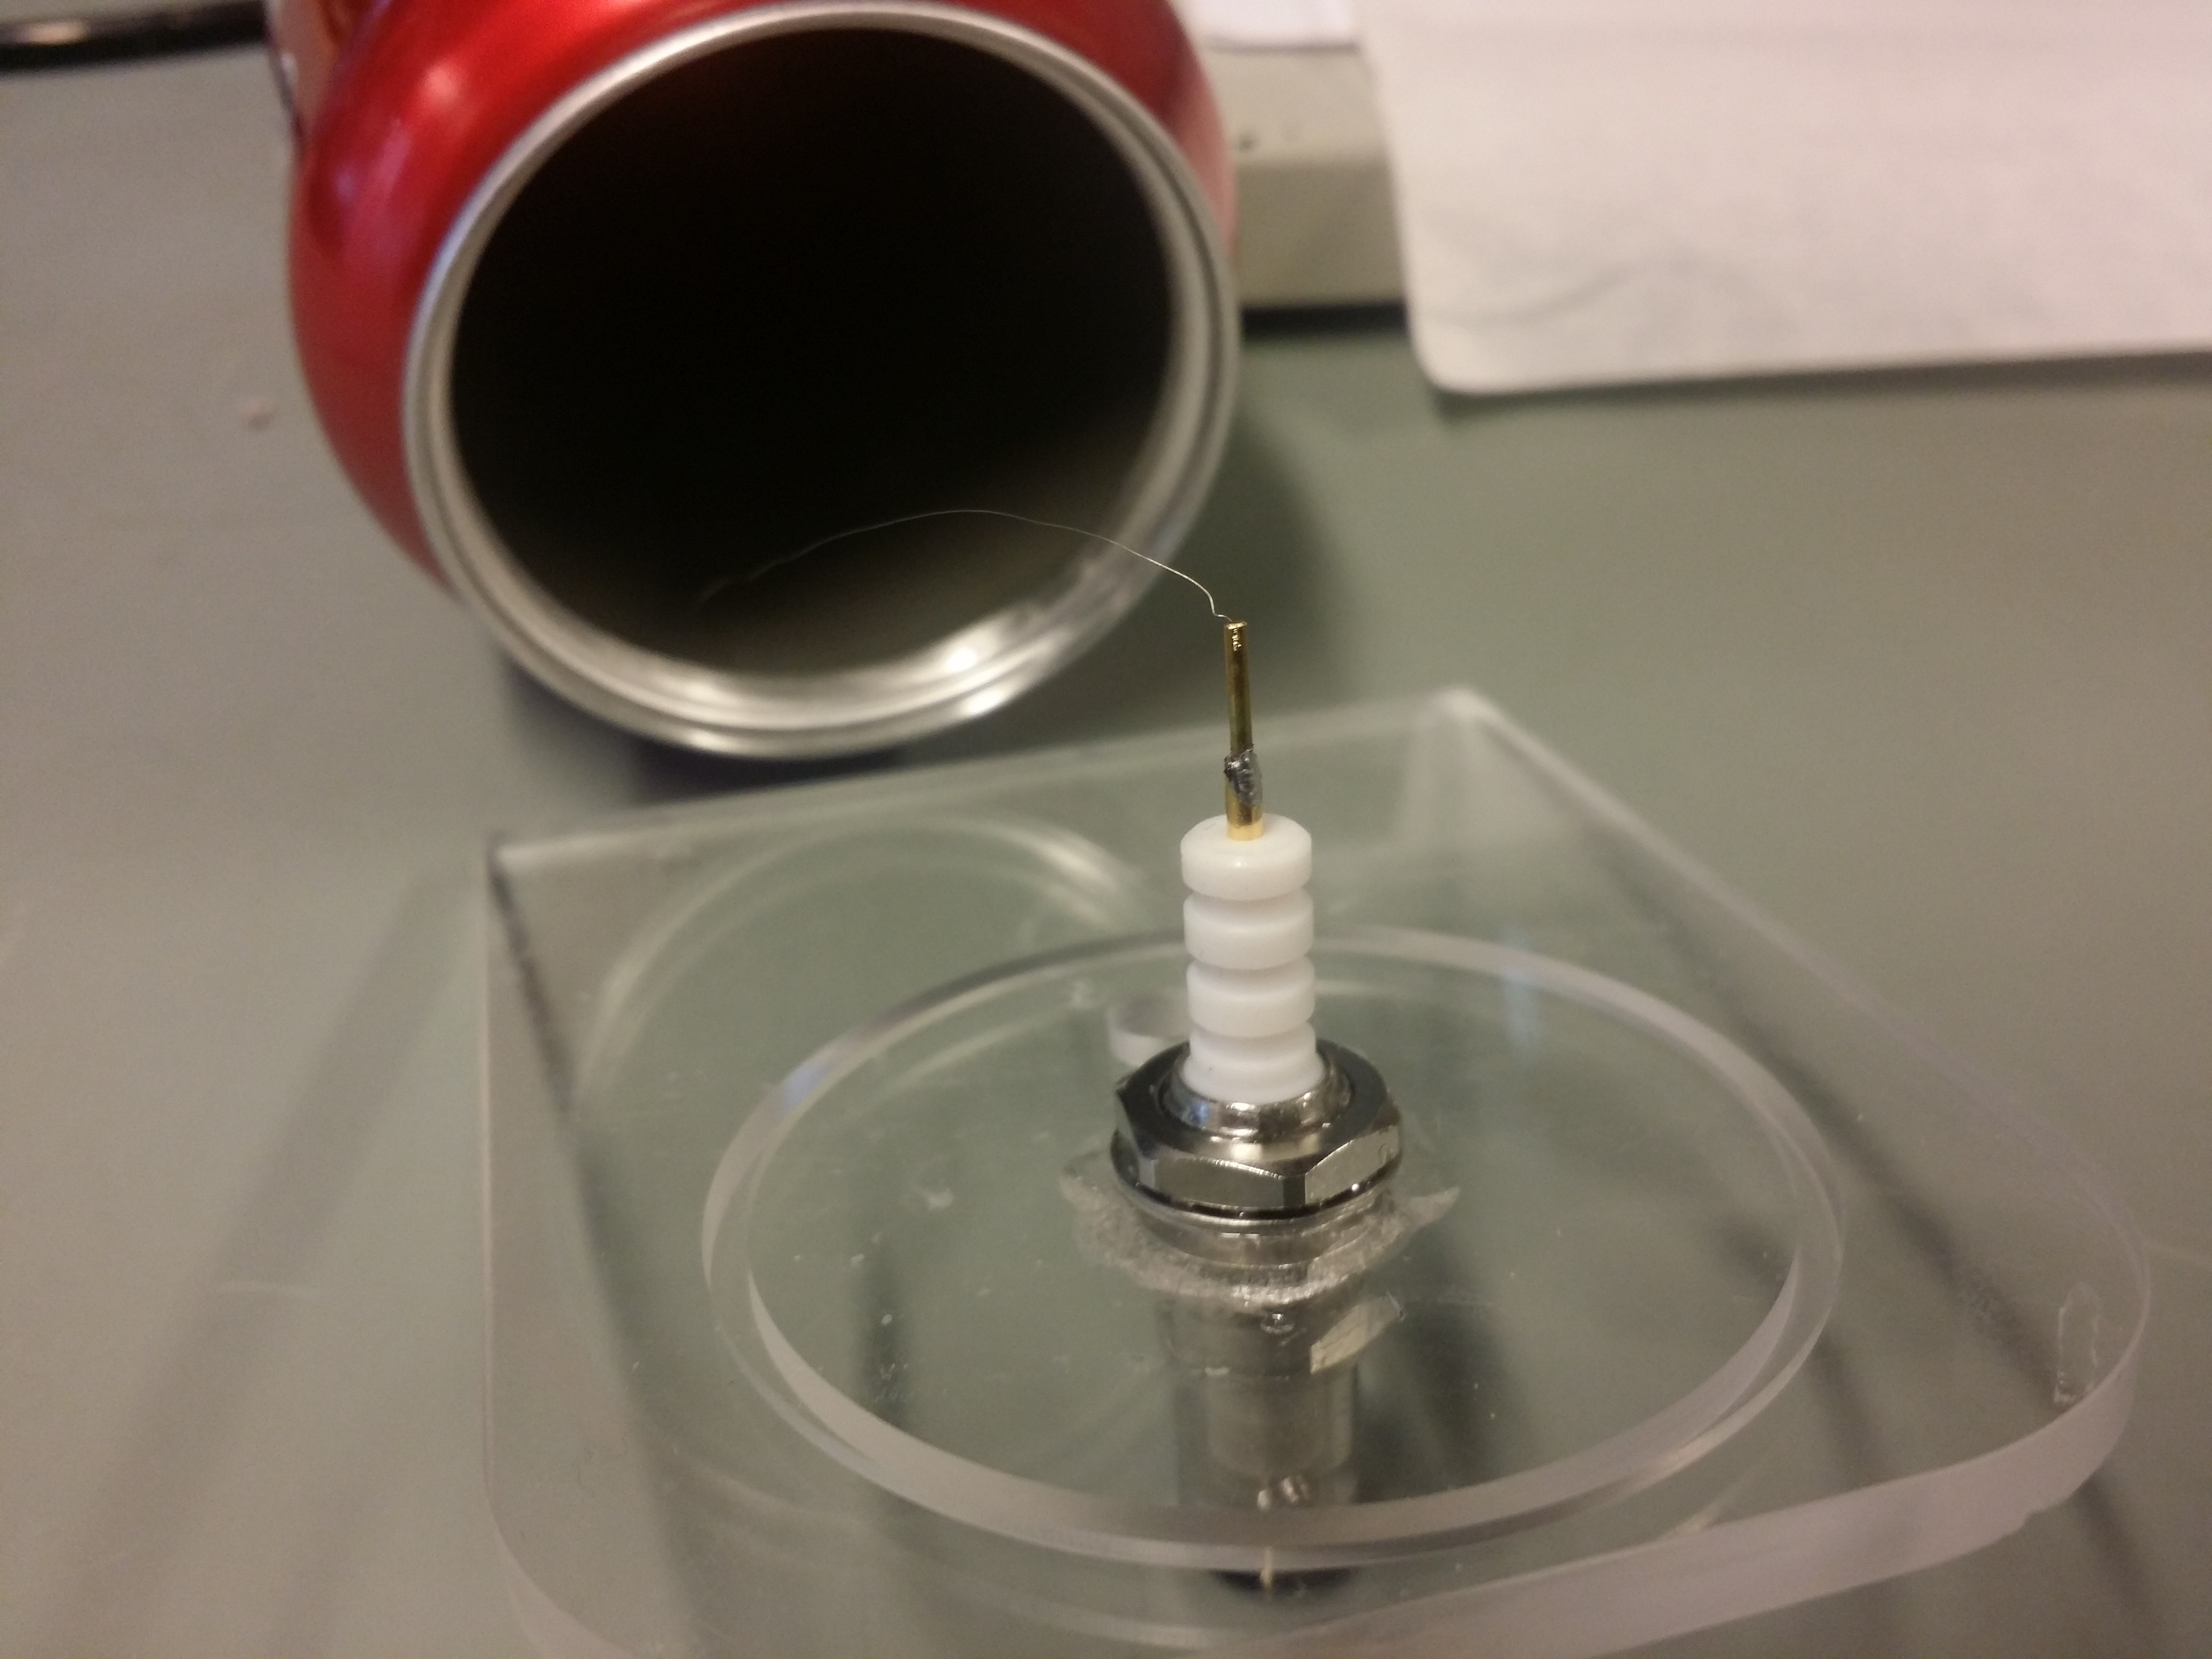
\includegraphics[width=\textwidth]{fig/IMG_20201117_121044.jpg}
\caption{The anode wire is soldered to the connector}
\label{fig:connector}
\end{subfigure}

\begin{subfigure}[t]{0.48\textwidth}
\centering
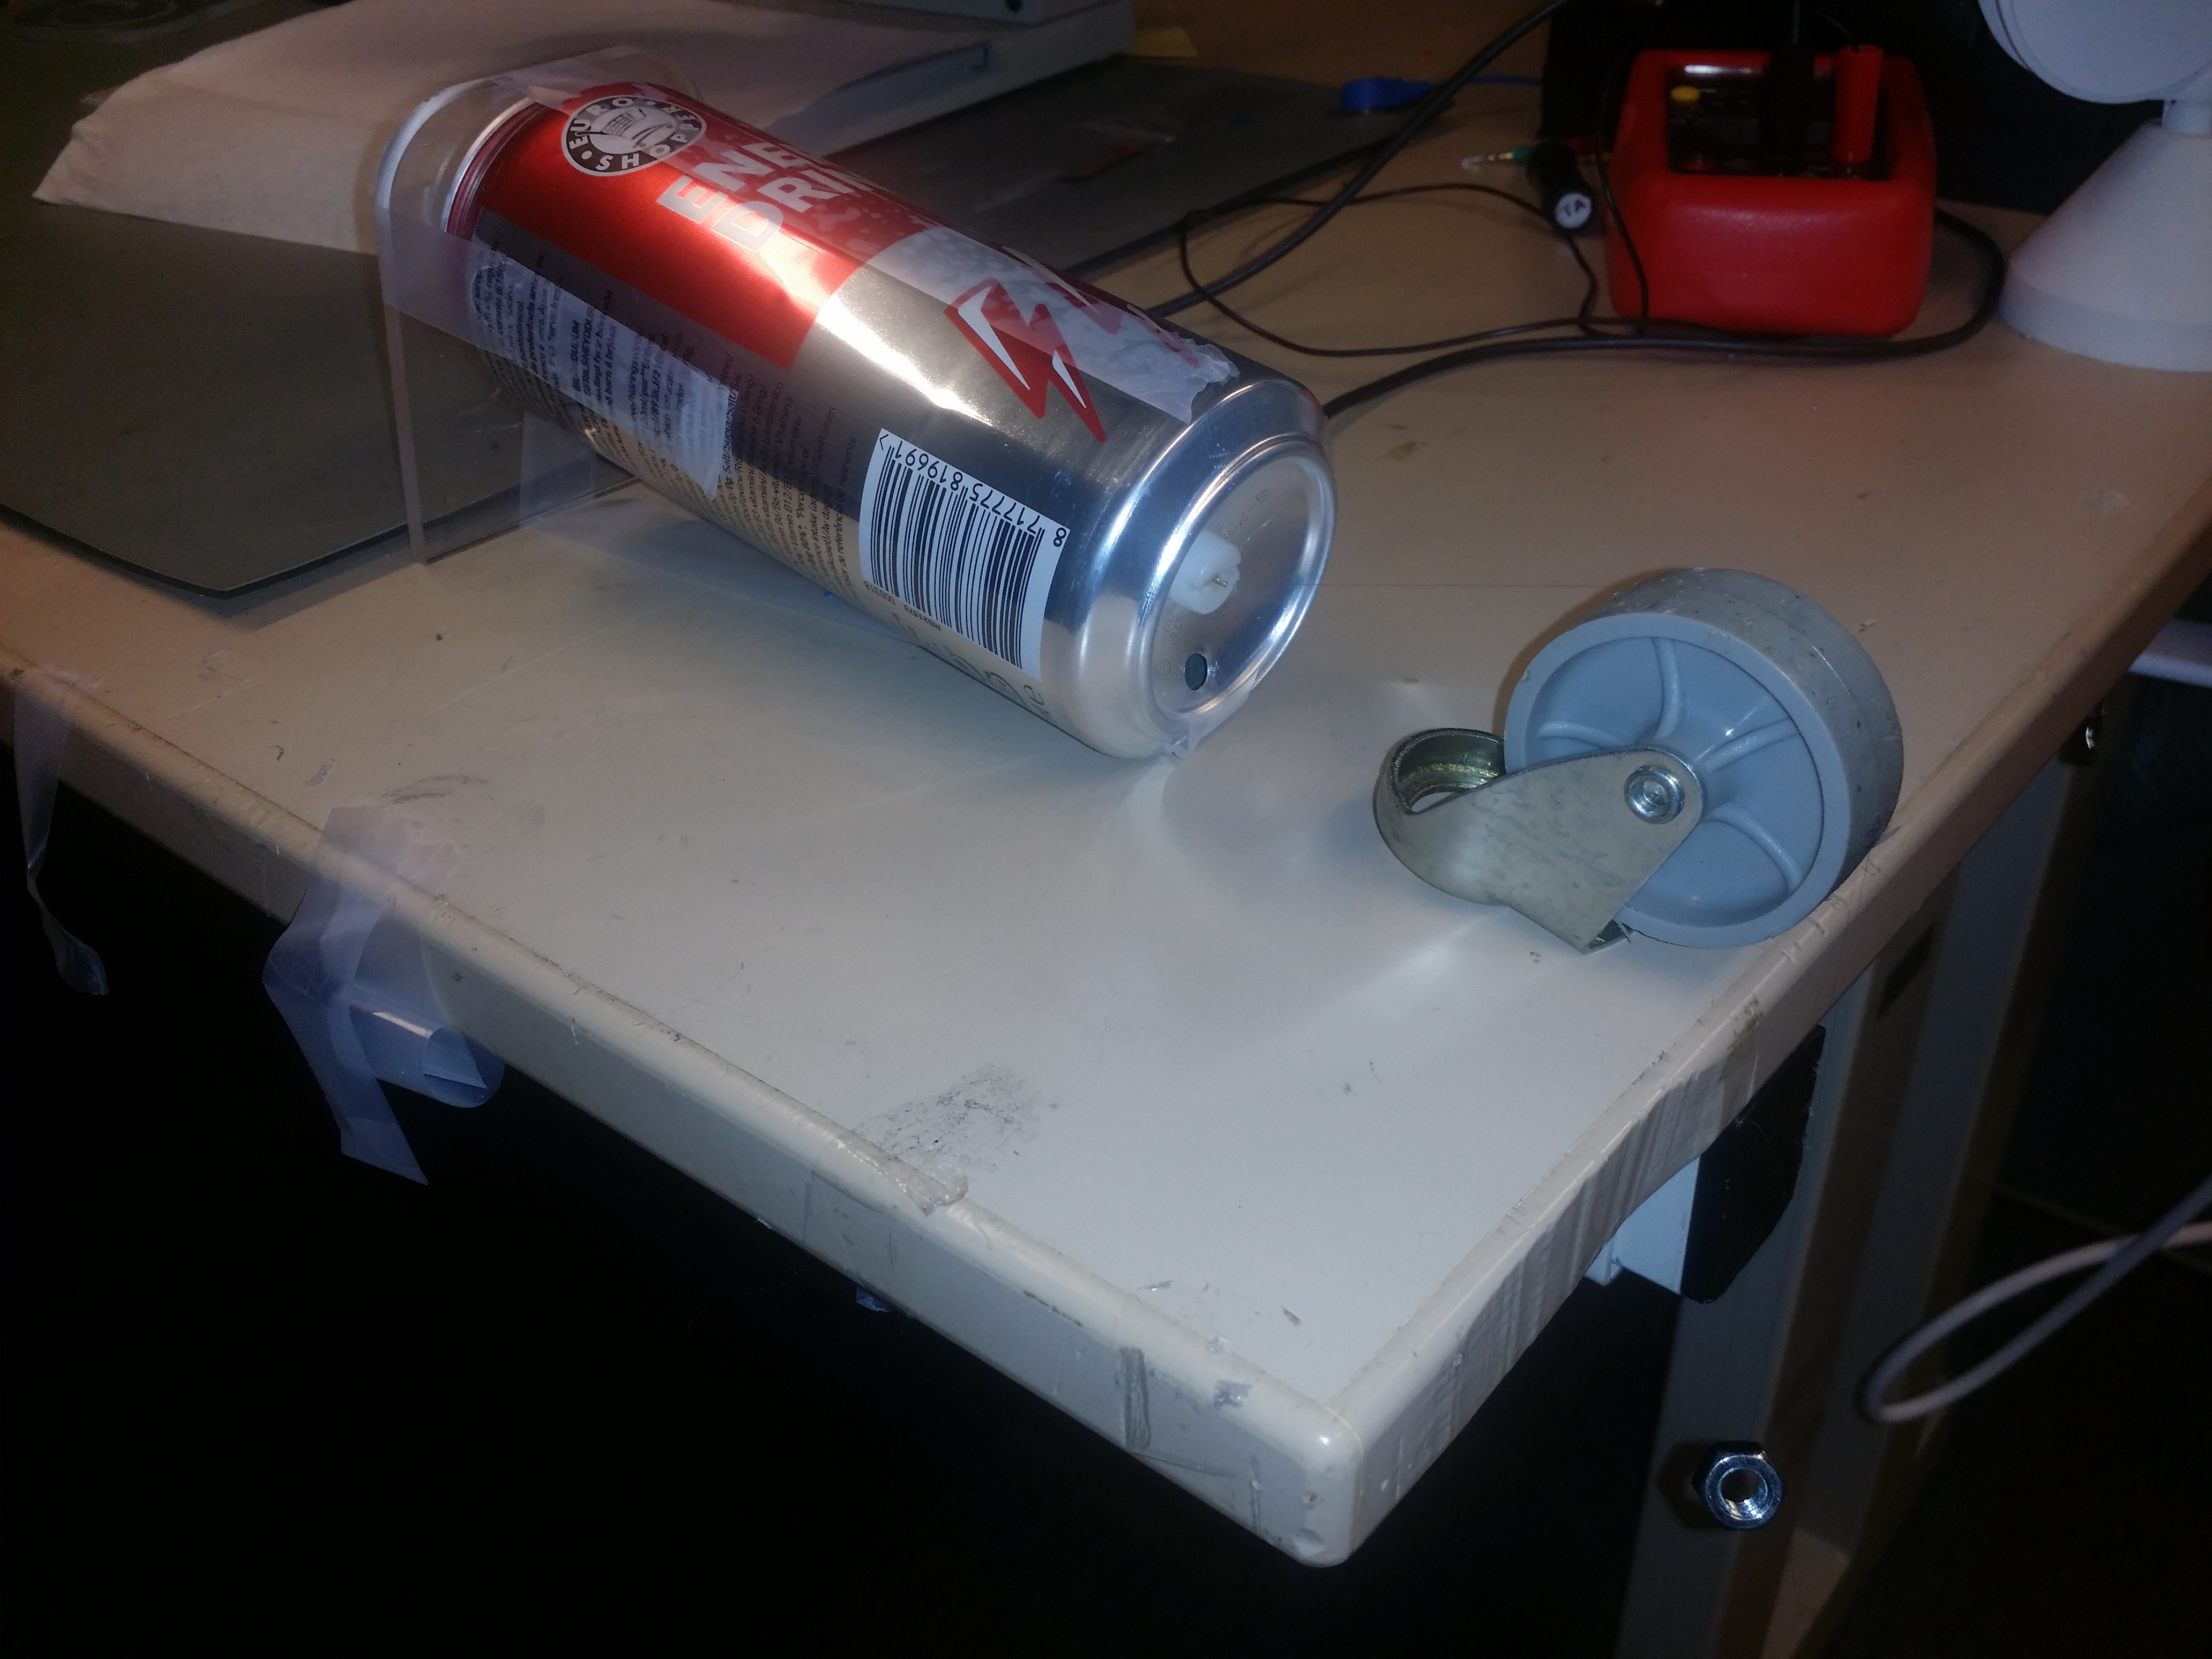
\includegraphics[width=\textwidth]{fig/IMG_20201123_104201.jpg}
\caption{Setup for tightening the anode wire}
\label{fig:tightening}
\end{subfigure}
%
\begin{subfigure}[t]{0.48\textwidth}
\centering
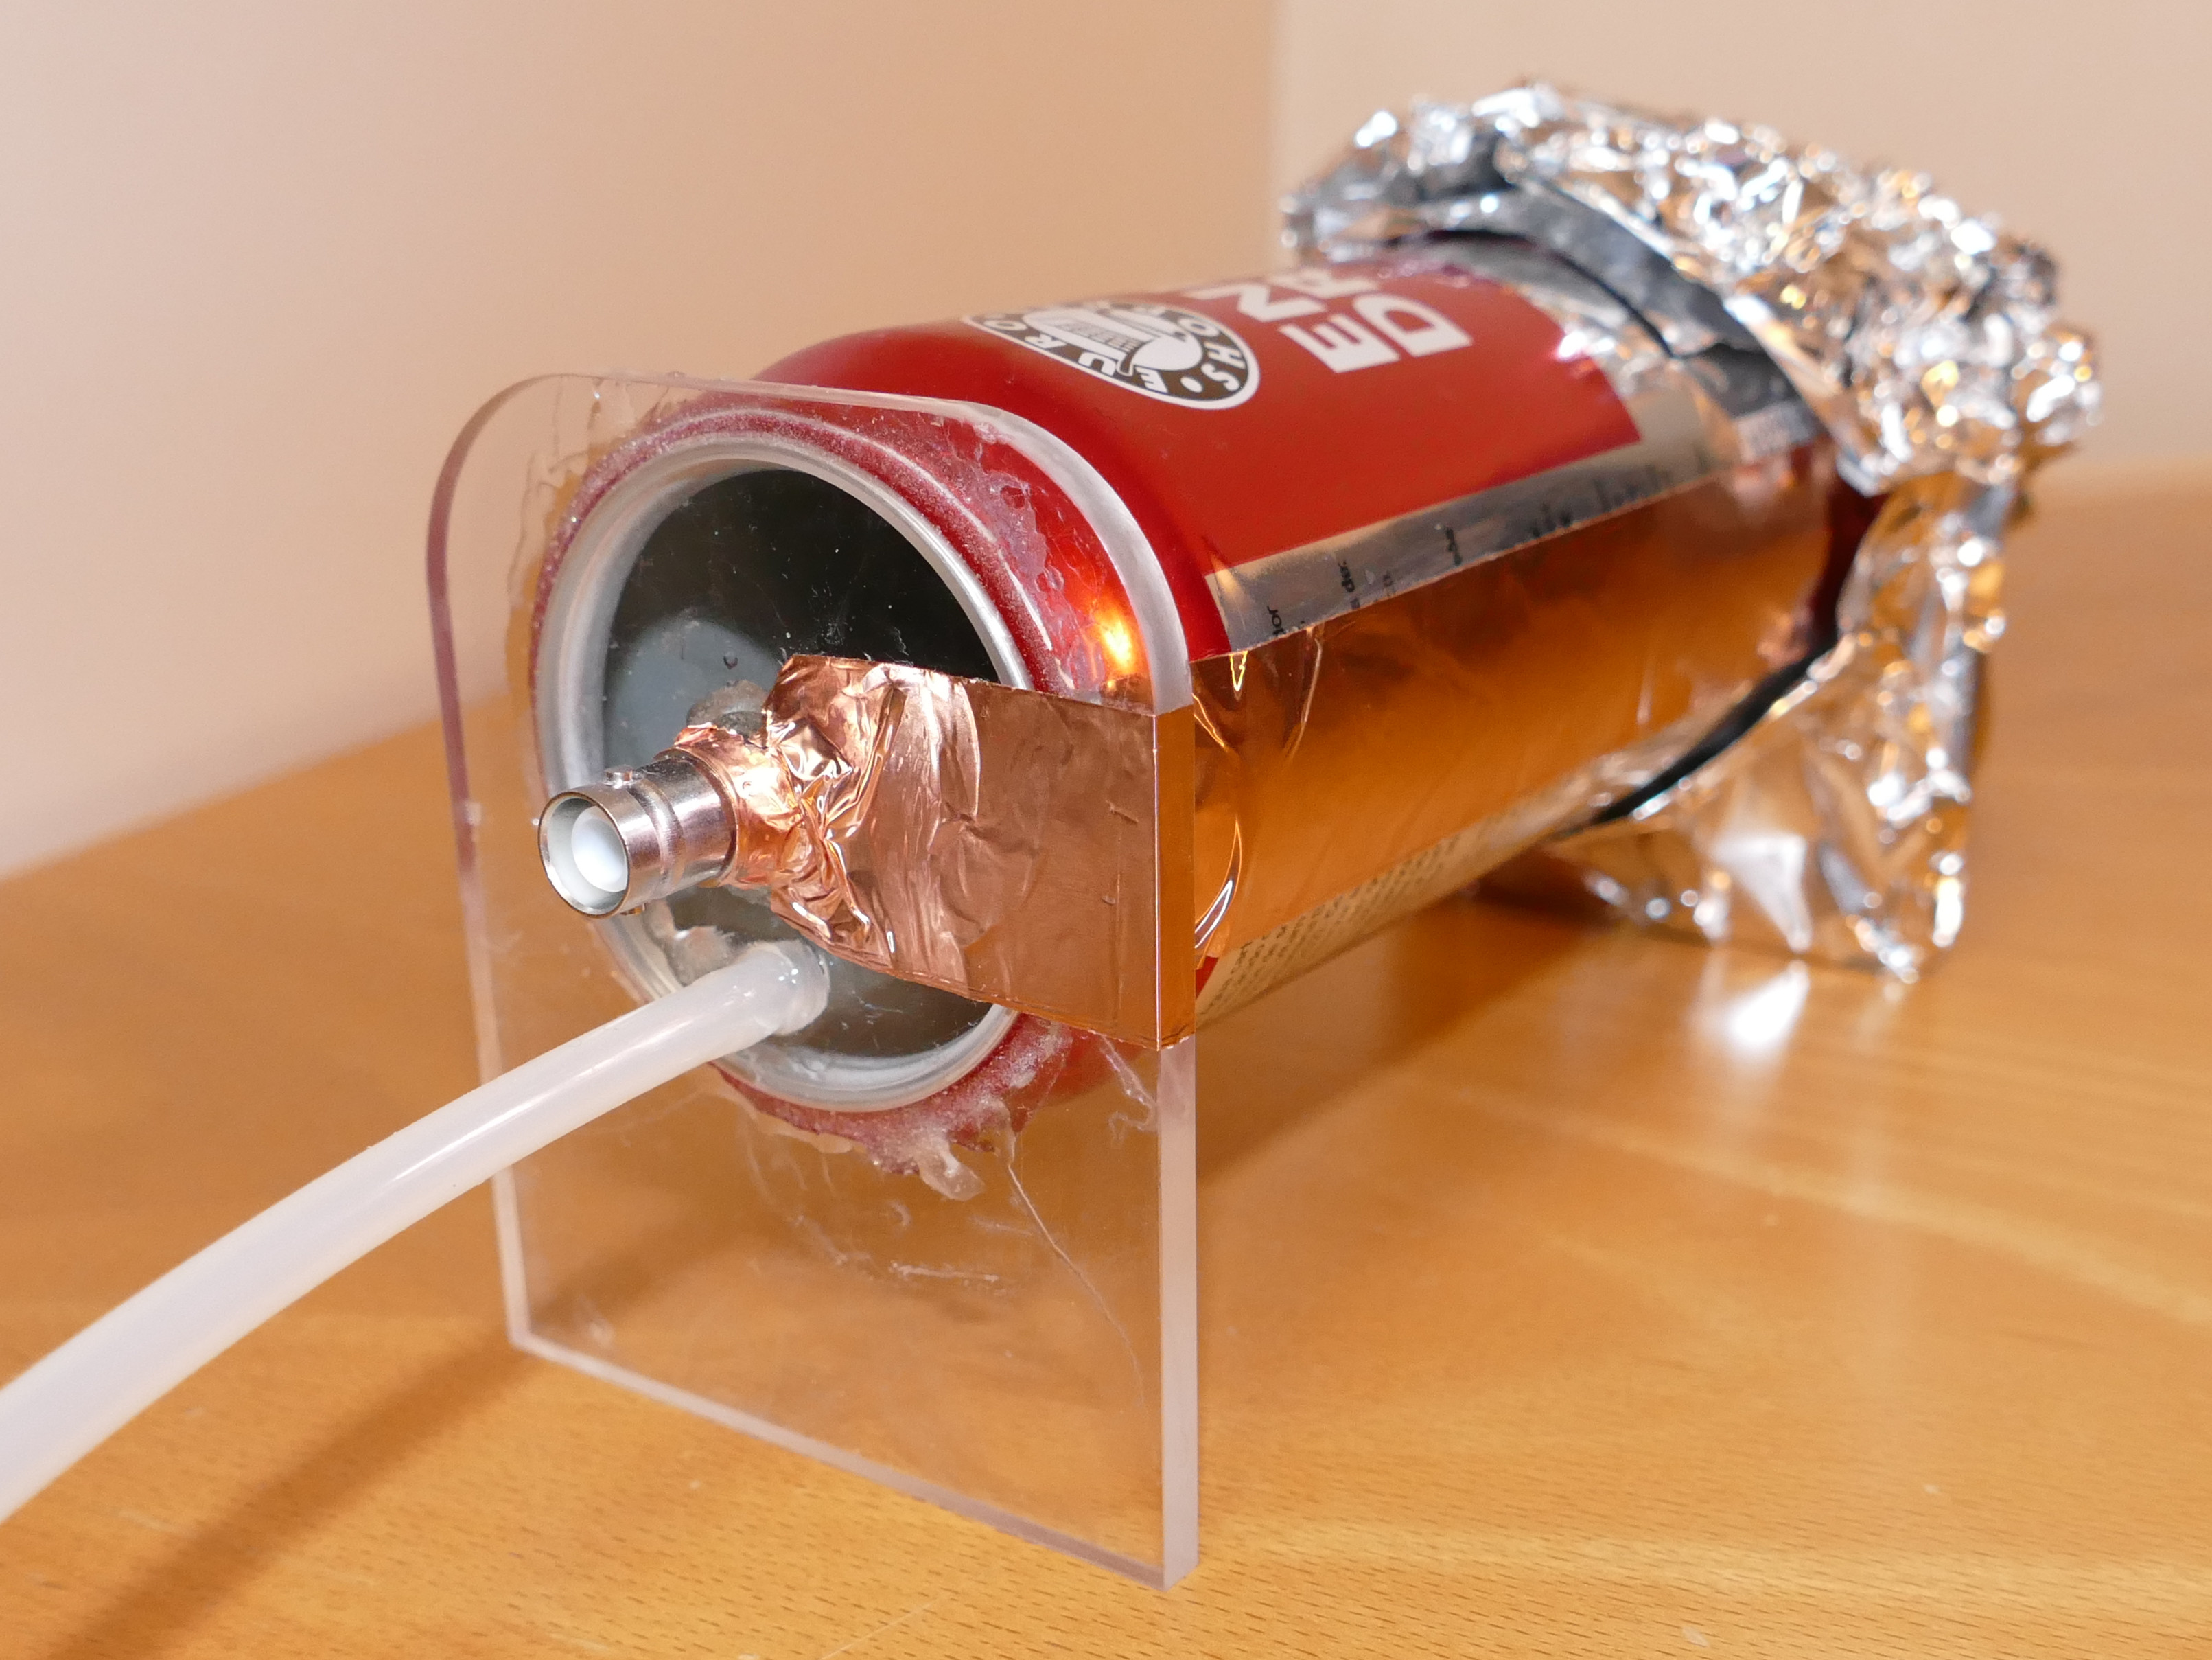
\includegraphics[width=\textwidth]{fig/P1170847-cropped.jpg}
\caption{Finished detector}
\label{fig:detector}
\end{subfigure}
%
\caption{Detector construction steps}
\end{figure}

The electric connection of the anode would be supplied by a high-voltage coaxial connector, which we attached to one of the
\href{https://en.wikipedia.org/wiki/Poly(methyl_methacrylate)}{plexiglass}
end caps with a nut and some epoxy glue.
The nut is sufficient to keep the connector in place, but the glue makes the connection airtight.
Once the connector was in place, we pushed the anode wire through the brass tube at the bottom of the can and pulled it out of the top of the can.
We then pushed the wire through the shorter brass tube and twisted it into a hook so that it stayed in place when we pushed the brass tube into the connector.
The electrical connection was then formed by soldering the brass tube and therefore also the wire to the connector as in figure \ref{fig:connector}
In this step one should be careful not to leave the end of the wire exposed from the solder, as such a sharp tip would cause high electric fields and therefore sparking.

Now the wire was in place, but it had to be tightened.
This was accomplished by taping the top cap to the can, knotting the wire around a nut and placing the wire over a wheel, as in figure \ref{fig:tightening}.
We then secured the tightening by soldering the wire to the brass tube, and then we cut the remaining wire.
In this step one should be careful to solder only as long as is needed for the solder to melt, as heating the wire for too long will cause it to break, as happened once during the manufacturing of this detector.
In the case of such an incident, a new wire has to be soldered to the high voltage connector.

Now the wire was in place, and the detector had to be sealed.
We used large amounts of epoxy to attach the end caps, and office tape to hold the caps in place.
In this step one should wait for the epoxy to dry properly before removing the top cap, as otherwise the cap may move and break the strained anode wire.
Once the epoxy of the caps was dry, we added some more to ensure airtightness, and then attached a pipe to the hole on each of the end caps.

Finally we brushed one side of the can with sandpaper and attached a piece of copper tape so that it went all the way to the shielding of the high voltage connector.
This established an electrical connection between the ground and the can.
It should be noted that the copper tape should be put on a different side than on which the radiation source is placed, as the copper tape would otherwise absorb some of the radiation.
A piece of aluminum foil was put over the bottom of the can to provide additional shielding from electromagnetic interference, as the end of the anode wire slightly extrudes from within the can.



\clearpage
\subsection{Calibration}
\label{setup_calibration}
The detector and readout electronics had to be calibrated to establish a relationship between the channels of the multichannel analyzer and the energies of the incoming radiation.
The setup consisted of an
\href{https://iseg-hv.com/en/products/detail/NHR}{Iseg NHR 42 60r}
high voltage power supply,
\href{https://www.ortec-online.com/products/electronics/preamplifiers/142a-b-c}{Ortec 142}
pre-amplifier,
\href{https://www.ortec-online.com/products/electronics/amplifiers/855}{Ortec 855}
dual spectral amplifier,
\href{https://www.amptek.com/products/multichannel-analyzers/mca-8000d-digital-multichannel-analyzer}{Amptek MCA-8000D}
digital multichannel analyzer and
\href{https://teledynelecroy.com/oscilloscope/wavesurfer-3000z-oscilloscopes/wavesurfer-3024z}{Lecroy WaveSurfer 3024z} oscilloscope (200 MHz).
The electrical connections of the setup used for both calibration and the measurements are illustrated in figure \ref{fig:connections}, except that for the electronics calibration the oscilloscope was connected directly to the output of the pulser.

\begin{figure}[ht!]
\centering
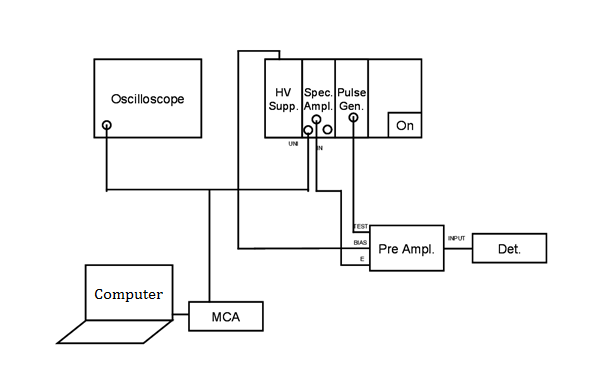
\includegraphics[width=\textwidth]{fig/instructions/connections.png}
\caption{Electrical connections of the setup \cite{instructions}}
% TODO draw own one with vector graphics}
\label{fig:connections}
\end{figure}

\FloatBarrier
The first step was the calibration of the multichannel analyzer to the collected charge.
This was done by setting the bias voltage to zero and attaching a pulse generator to the amplifier input, and an oscilloscope and the multichannel analyzer to its output, as in figure \ref{fig:pulser_setup}.
The voltage over a capacitor is defined by the equation $V = \frac{Q}{C}$, where $Q$ is the collected charge, $C$ is the capacitance of the pre-amplifier.
Therefore the collected charge is defined by $Q = CV$, where $V$ is the output pulse height measured with the oscilloscope.
The pulse height was determined by comparing the value of an exponential fit at the peak time to the average voltage before the pulse.
These are illustrated in figure \ref{fig:cal_trace}.

\begin{figure}[ht!]
\centering
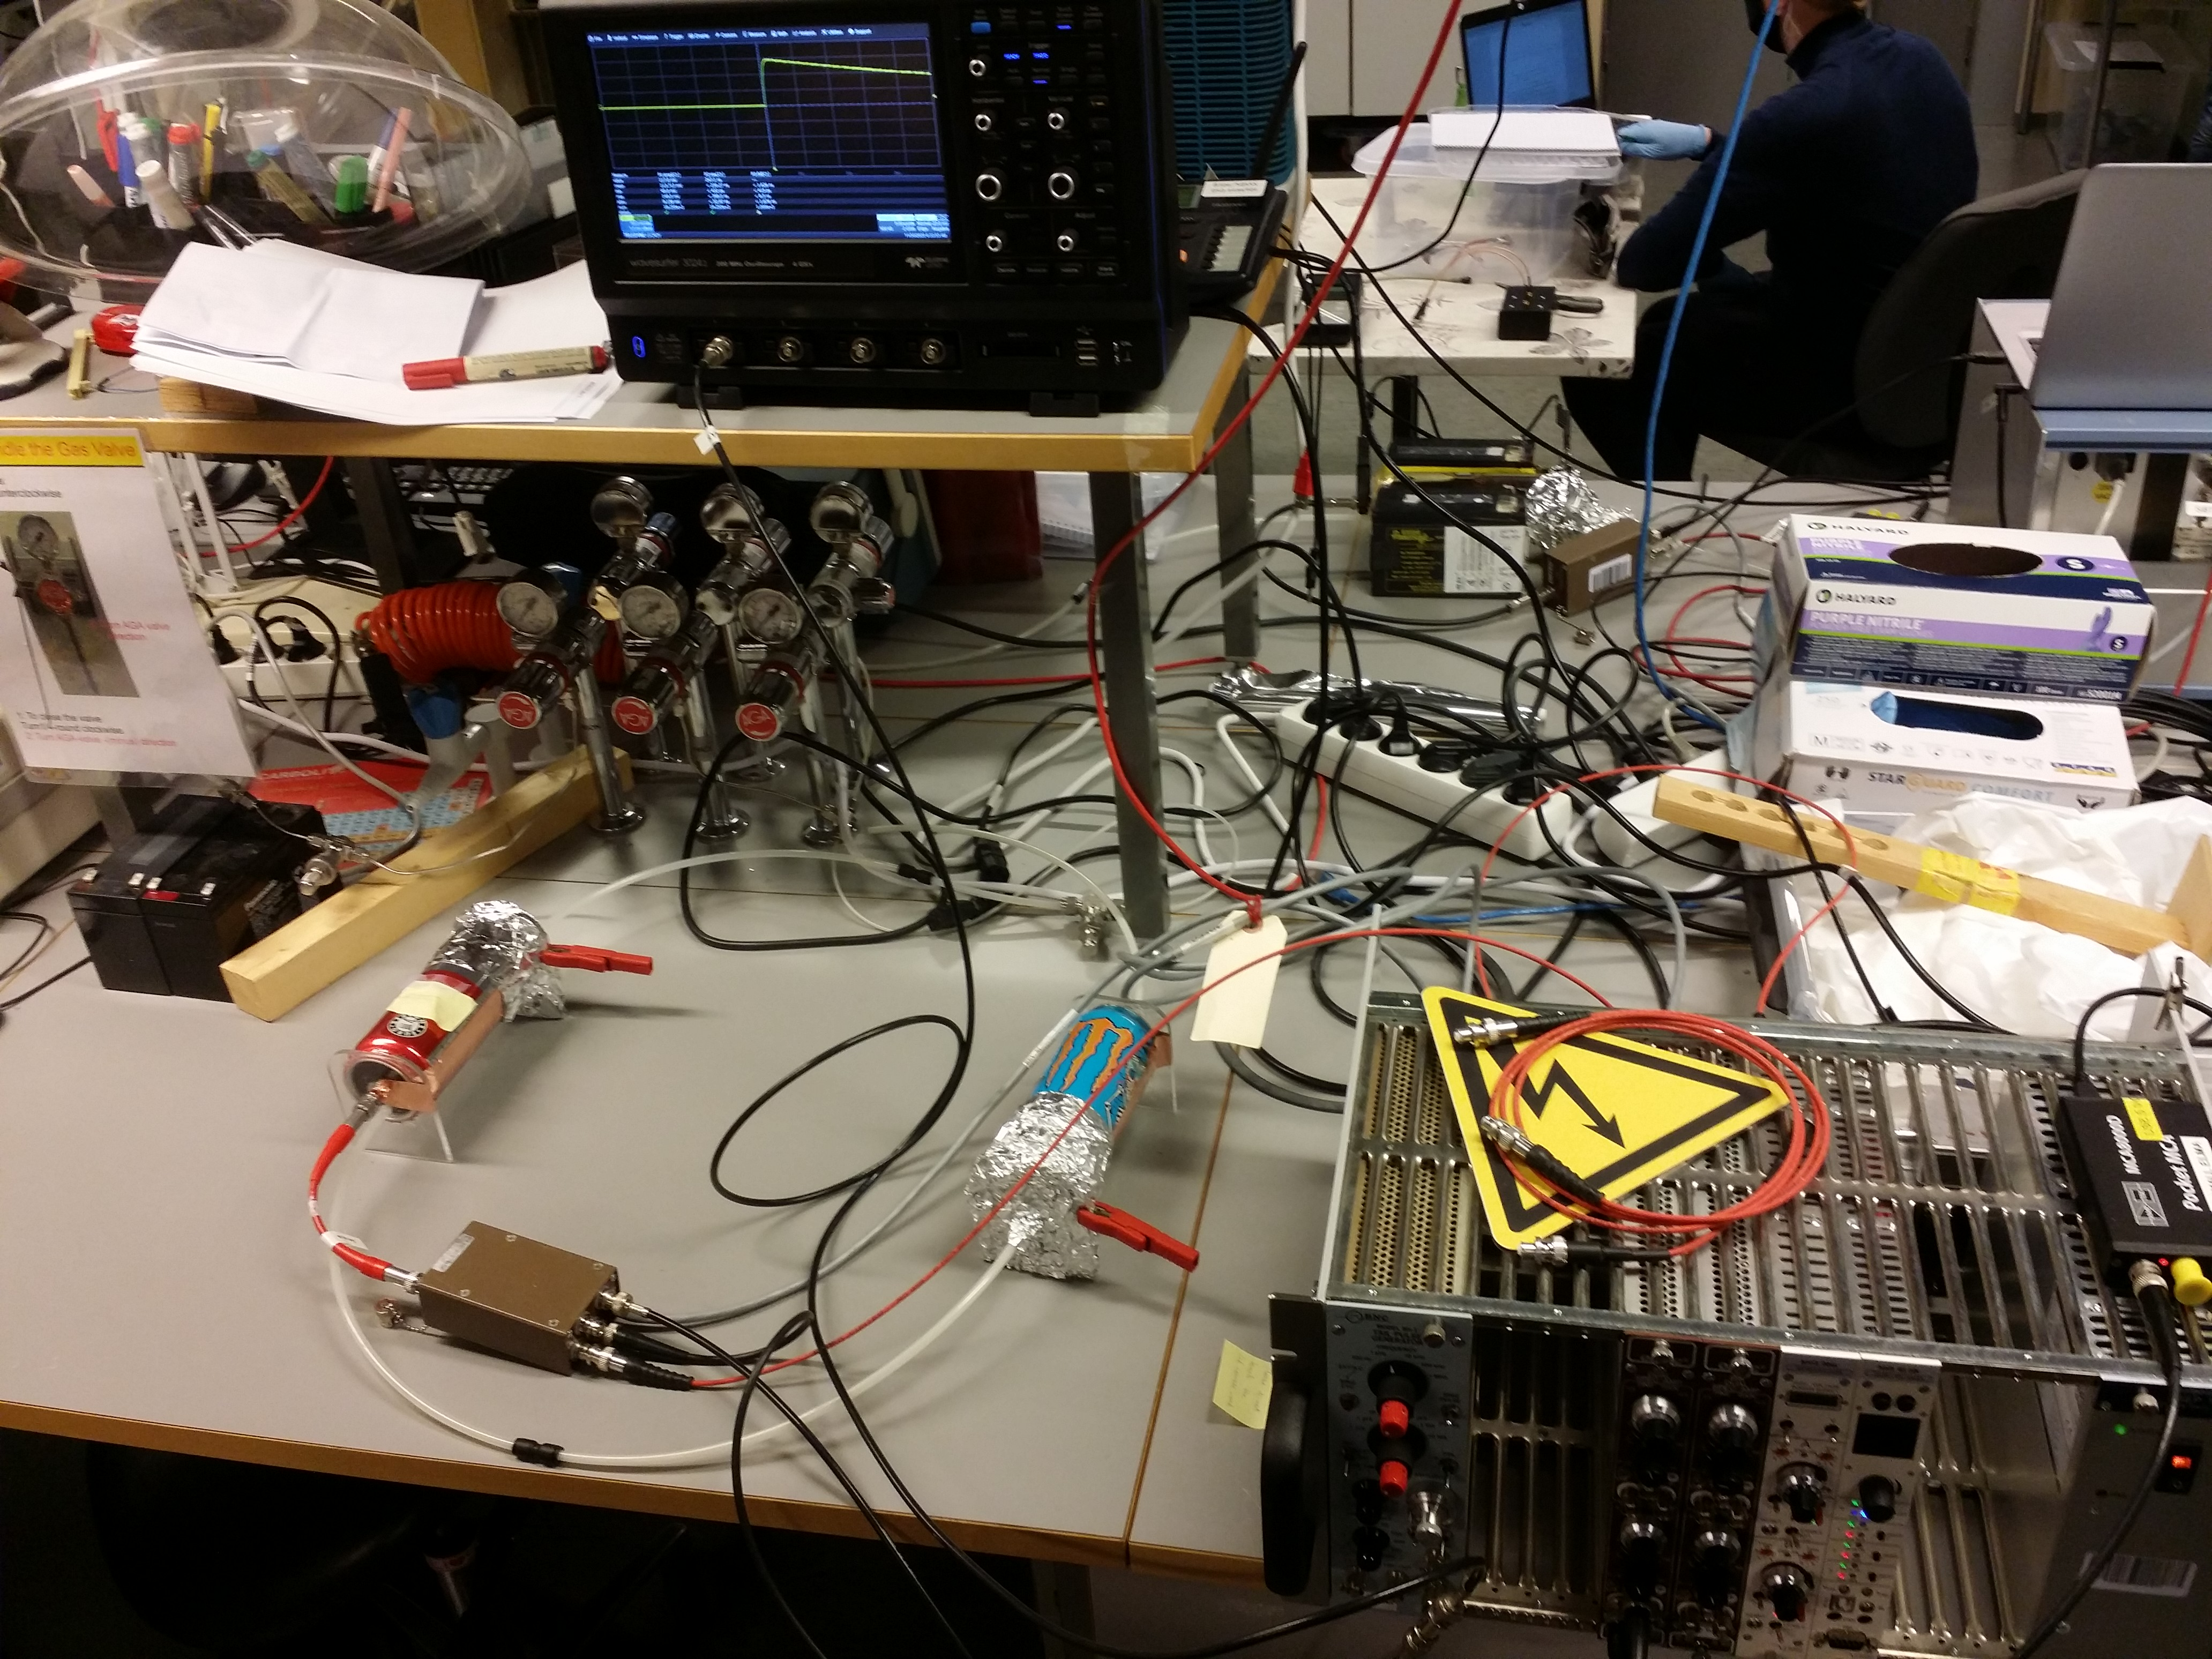
\includegraphics[width=0.8\textwidth]{fig/IMG_20201130_135000.jpg}
\caption{Setup for testing with an external pulser}
\label{fig:pulser_setup}
\end{figure}

\begin{figure}[ht!]
\centering
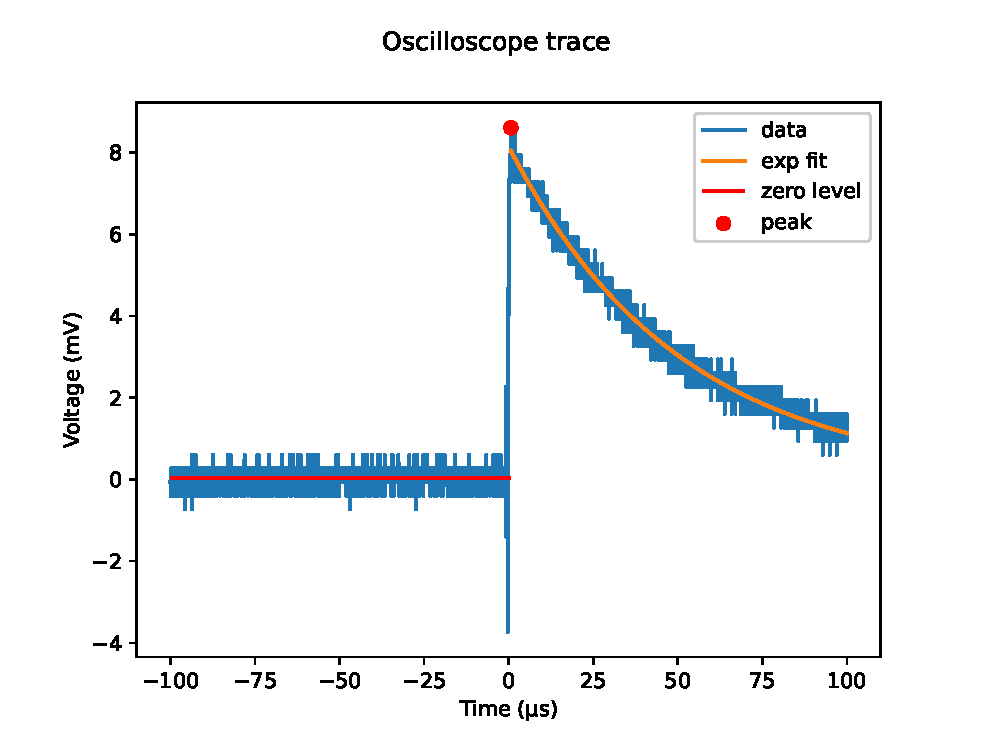
\includegraphics[width=\textwidth]{fig/python/calibration_trace.eps}
\caption{An oscilloscope trace for the calibration}
\label{fig:cal_trace}
\end{figure}



\FloatBarrier
\subsection{Measurements with radiation sources}
\label{setup_testing}
For the testing with radiation sources the electrical connections were the same as for the calibration, except that the pulse generator was removed and that the oscilloscope was attached to the output of the spectral amplifier.
The detector was placed within a lead shielding that consisted of two lead-acid batteries, and the radioactive source was placed on top, as in figure \ref{fig:setup_testing}.
For the $^{241}$Am source we had to use a thick metal sheet with a thin slit as a collimator to reduce the intensity of the radiation.
Without the attenuator the pulses would pile up so that individual pulses would no longer be detectable separately for energy measurement.
Due to its different enclosure and higher activity, the $^{241}$Am source also required the use of additional lead shielding around the setup to prevent unnecessary user exposure to the radiation.

\begin{figure}[ht!]
\centering
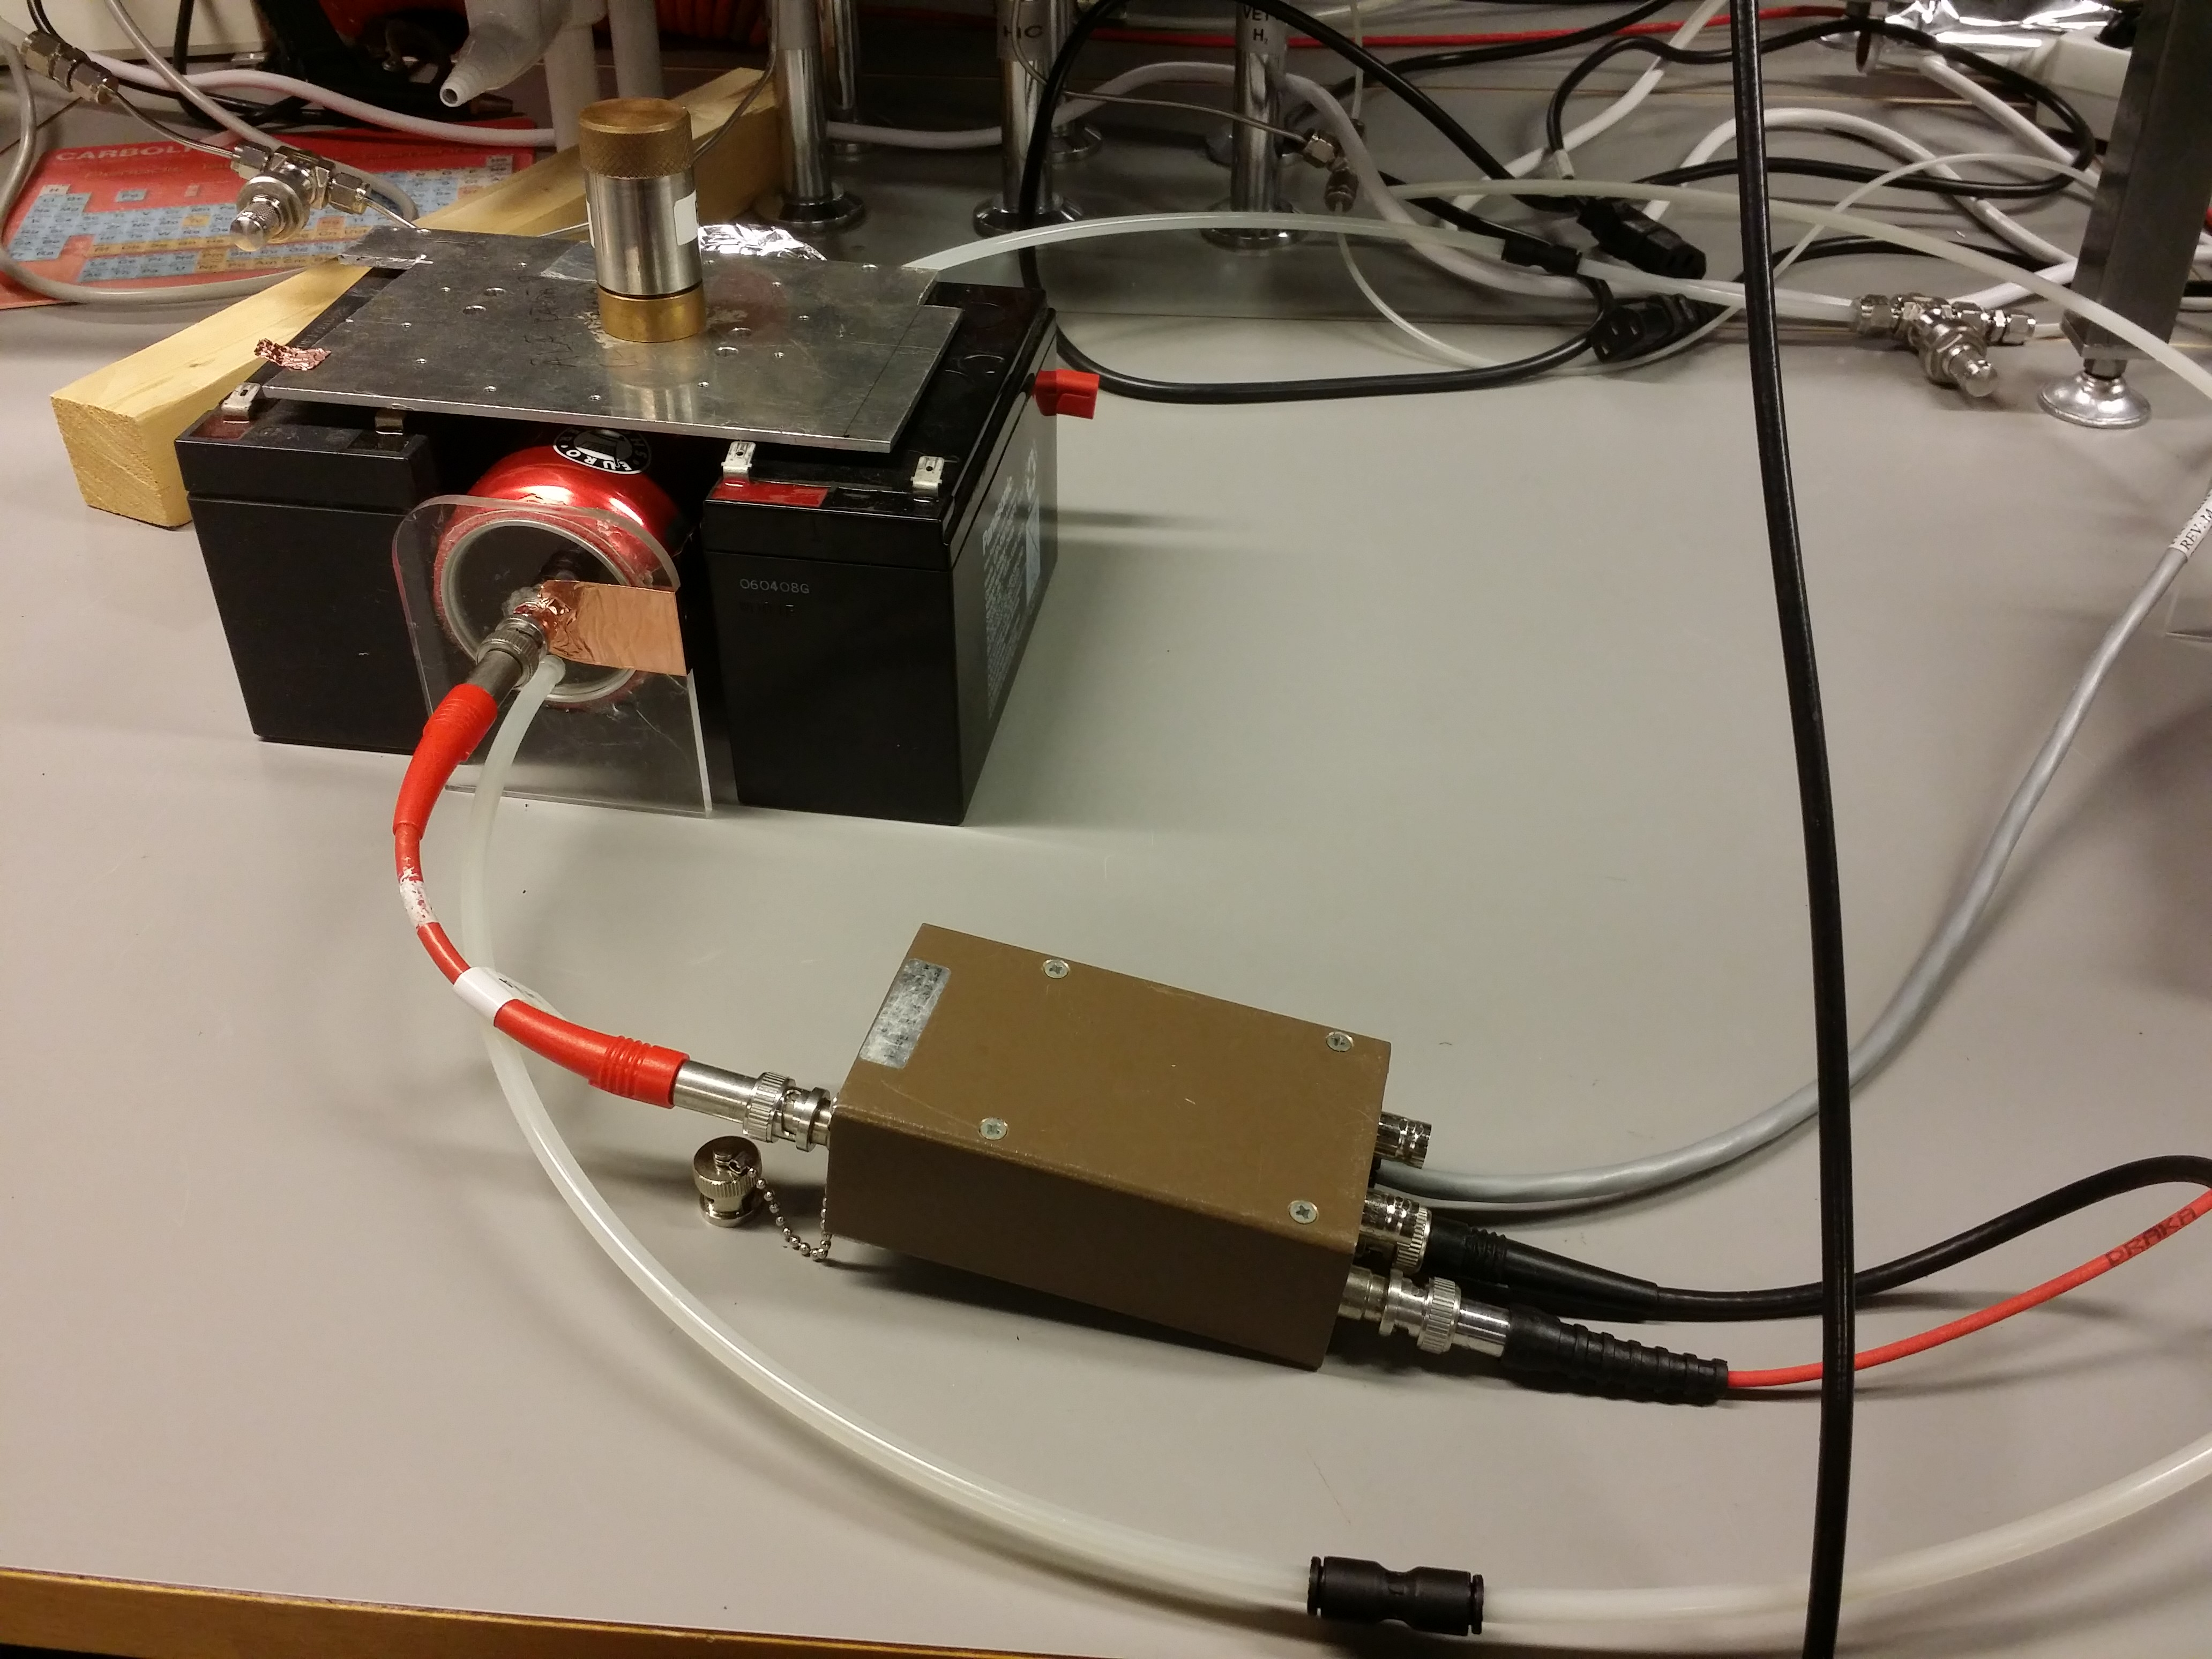
\includegraphics[width=0.8\textwidth]{fig/IMG_20201130_144418.jpg}
\caption{Setup for testing with an $^{55}$Fe source and the rack-mounted amplifier}
\label{fig:setup_testing}
\end{figure}



\clearpage
\section{Results and discussion}
\label{results}
In this chapter we discuss the measurement results of the setups described in chapter \ref{assembly}.
The code used for the data analysis is available in the GitHub repository. \cite{repo}


\subsection{Calibration}
\label{results_calibration}
By varying the voltage of the test pulse we get the relationship between the peak MCA channel and the collected charge as in \ref{fig:mca_calibration}.
The error bars represent the standard deviation of five measurements except for one data point which had four successful measurement and one data point which had only two due to technical issues.
To this data we can make the linear fit
\begin{equation}
Q = g \cdot \text{Channel}_\text{MCA} + h,
\end{equation}
and for the fit parameters we get the values $g = 1.46 \cdot 10^{-4} \pm 4.81 \cdot 10^{-7}$ pC/channel and $h = -1.04 \cdot 10^{-4} \pm 6.99 \cdot 10^{-5}$ pC.

\begin{figure}[ht!]
\centering
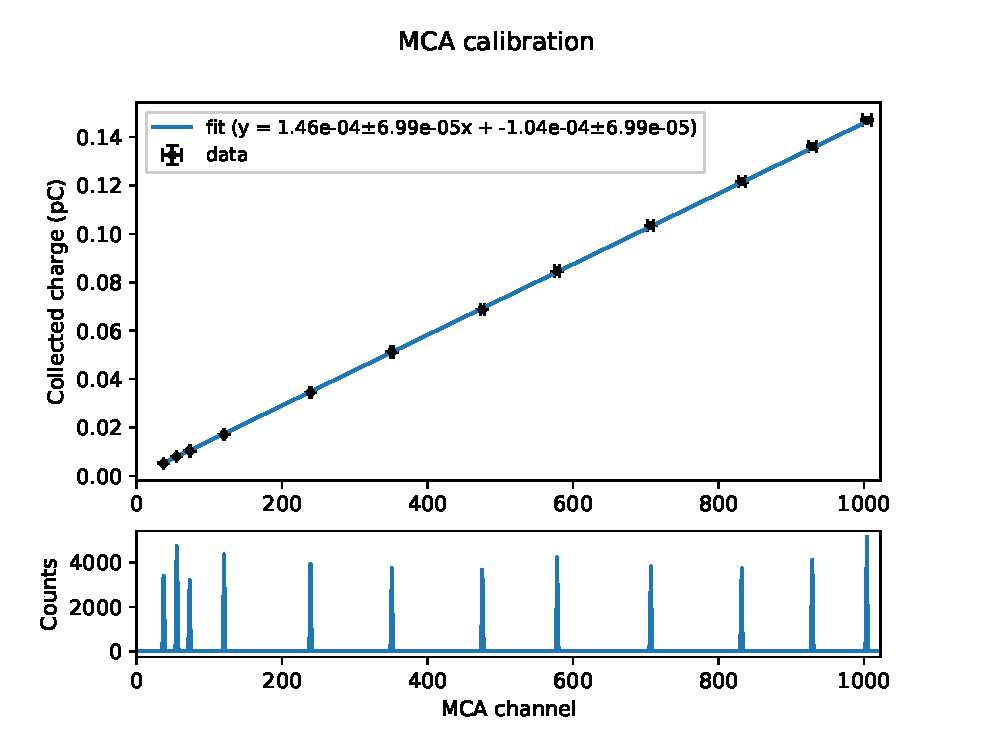
\includegraphics[width=\textwidth]{fig/python/mca_calibration.eps}
\caption{MCA calibration: collected charge as a function of the MCA channel with a linear fit, and a histogram of the measured detection counts}
\label{fig:mca_calibration}
\end{figure}

It should be noted that the pulse heights measured with the oscilloscope differred significantly from those set on the pulser.
The relationship between these is illustrated in figure \ref{fig:pulser_calibration}.

\begin{figure}[ht!]
\centering
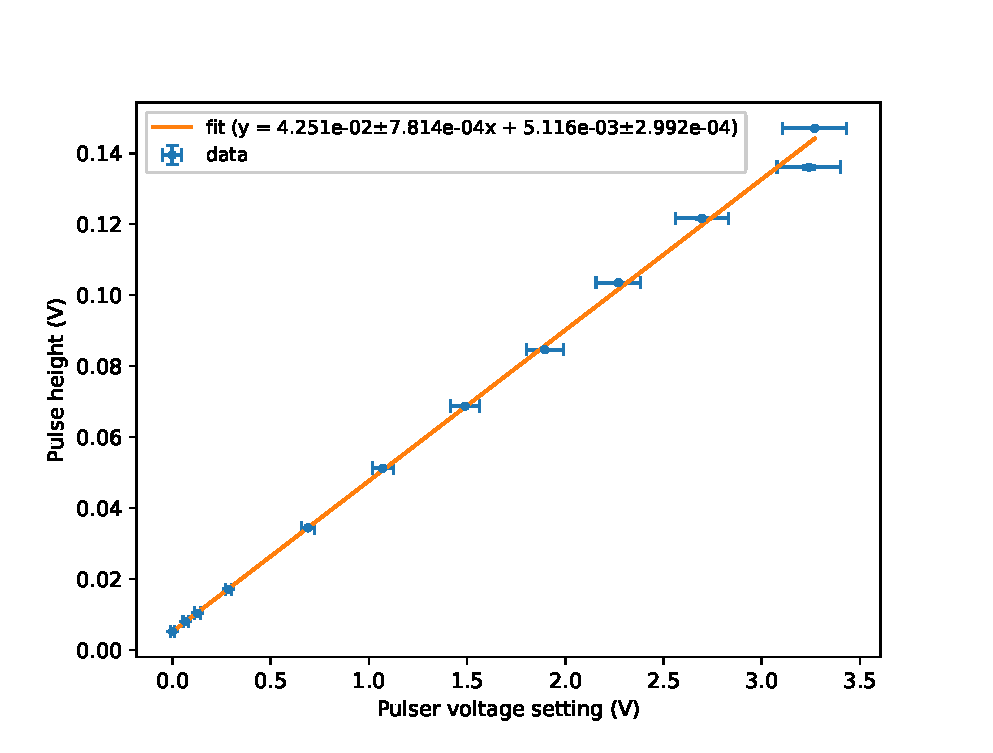
\includegraphics[width=\textwidth]{fig/python/pulser_calibration.eps}
\caption{Pulser calibration}
\label{fig:pulser_calibration}
\end{figure}


\clearpage
\subsection{High voltage sweep}
\label{results_hv}
To find the optimal settings for the detector we tested it with several voltages and gain values.
With the $^{241}$Am source we obtained the spectra in figure \ref{fig:am_scan_fits} and for the $^{55}$Fe source the data in figure \ref{fig:fe_scan_fits}.
For $^{55}$Fe the tested voltage range was 1603--2301 V, and for $^{241}$Am 1152--2301 V, as within this range suitable gain values were available to fit the signal within the range of the multichannel analyzer.

\begin{figure}[ht!]
\centering
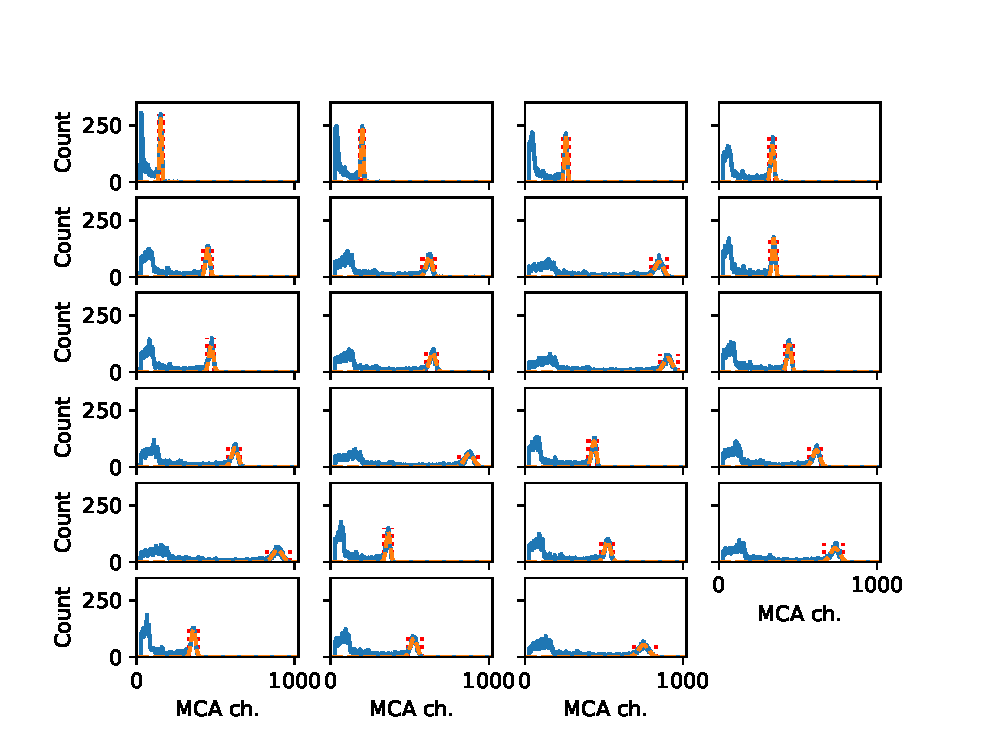
\includegraphics[width=\textwidth]{fig/python/am_scan_fits.eps}
\caption{$^{241}$Am voltage scan data}
\label{fig:am_scan_fits}
\end{figure}

\begin{figure}[ht!]
\centering
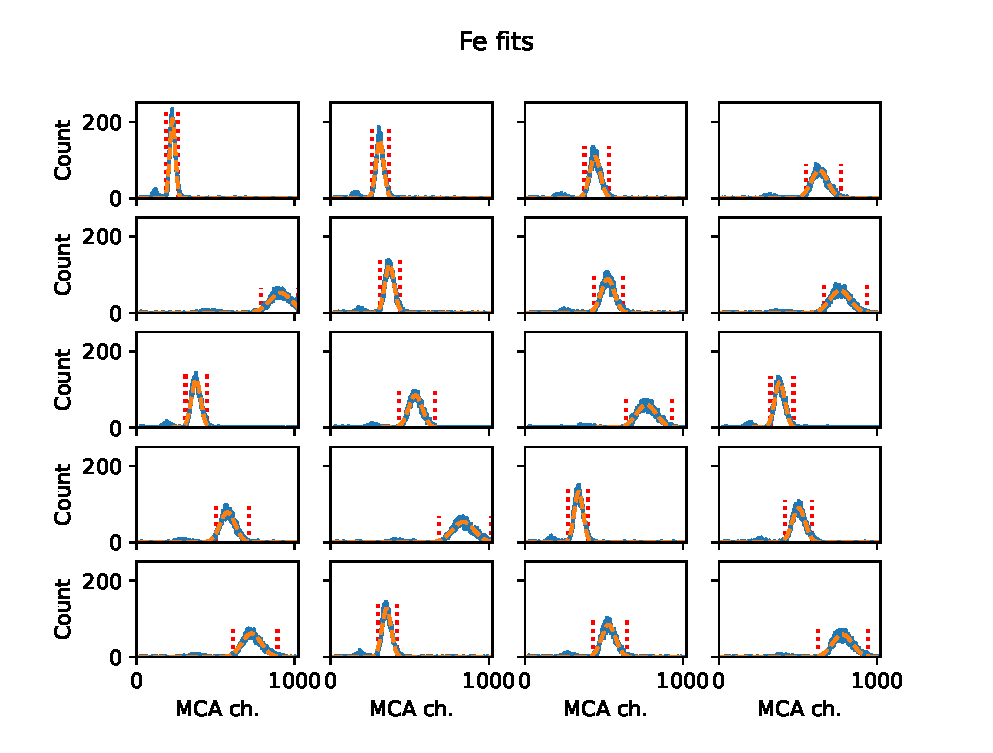
\includegraphics[width=\textwidth]{fig/python/fe_scan_fits.eps}
\caption{$^{55}$Fe voltage scan data}
\label{fig:fe_scan_fits}
\end{figure}

\begin{figure}[ht!]
\centering
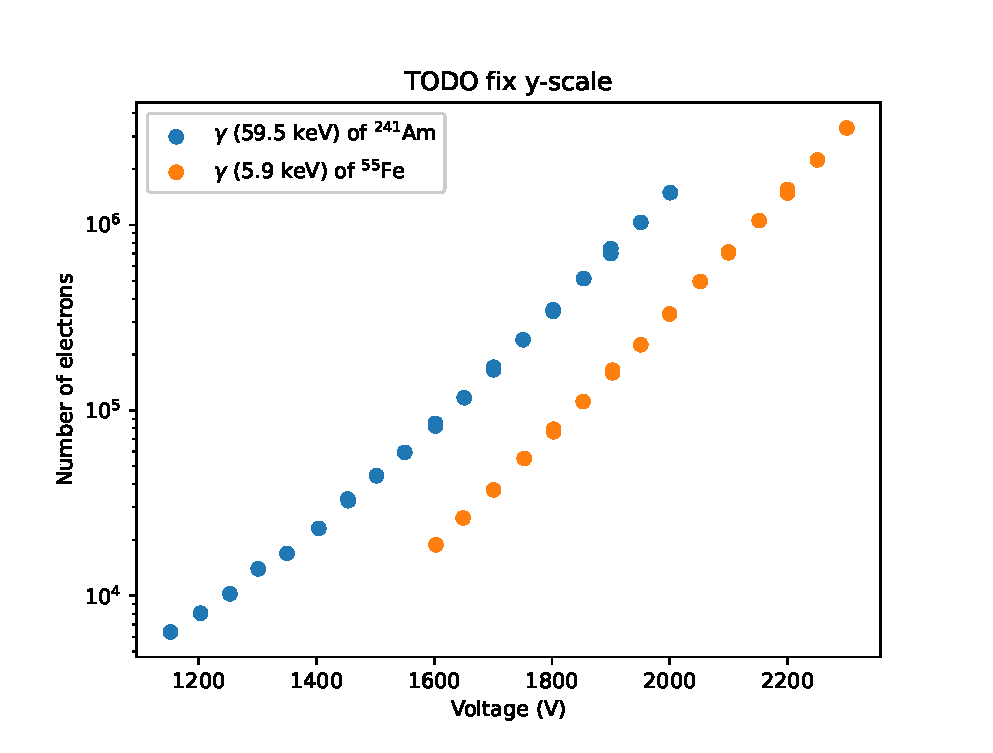
\includegraphics[width=\textwidth]{fig/python/hv_scans.eps}
\caption{Measured charge as a function of voltage}
\label{fig:hv_scans}
\end{figure}

\FloatBarrier
For the $^{55}$Fe source the measured charge increases exponentially for the entire measured range.
On the other hand, for the $^{241}$Am there is a change of voltage dependence at about 1500 V.
Consequently it appears that the detector reaches the desired proportional region at about 1500 V.

\begin{figure}[ht!]
\centering
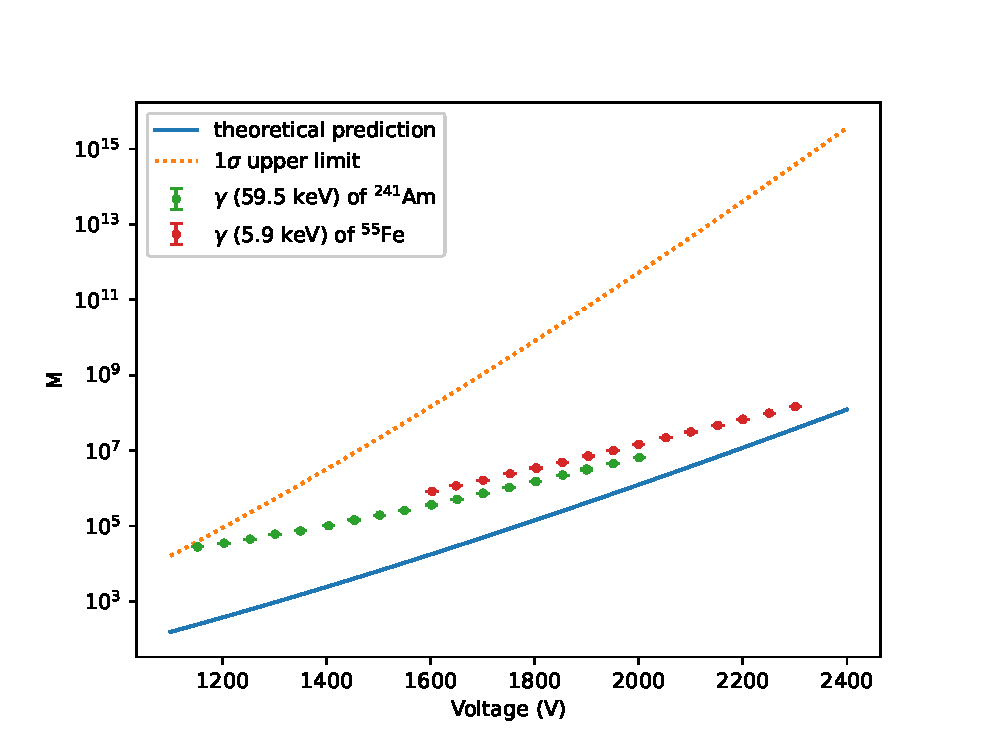
\includegraphics[width=\textwidth]{fig/python/gas_mult.eps}
\caption{Gas multiplication factor as a function of voltage}
\label{fig:gas_mult}
\end{figure}

\begin{figure}[ht!]
\centering
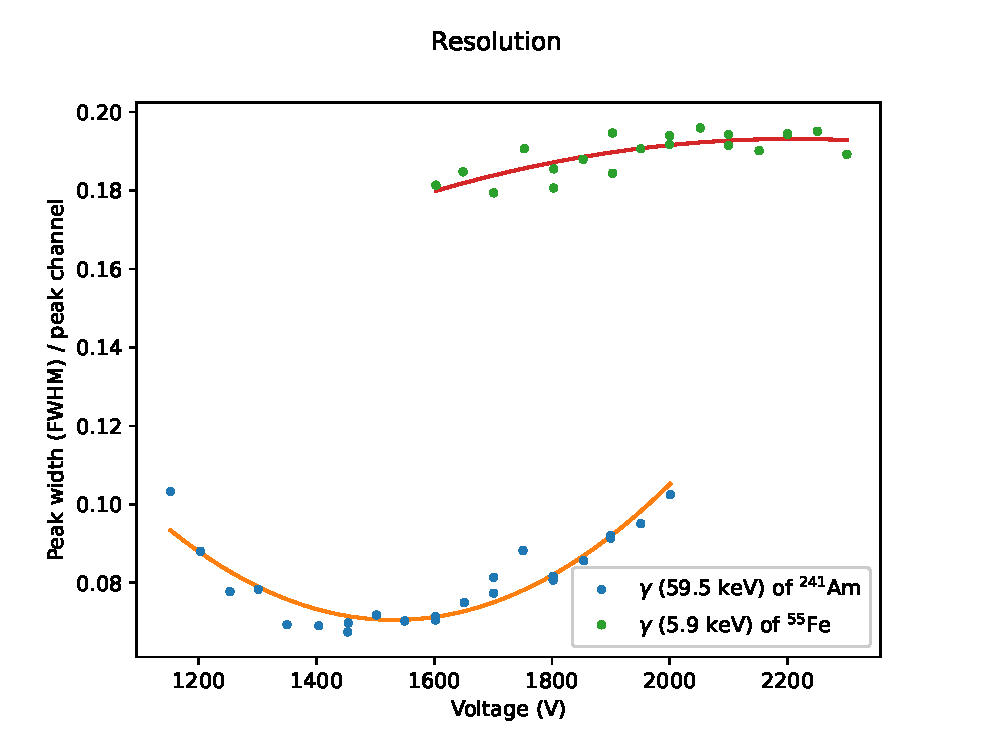
\includegraphics[width=\textwidth]{fig/python/resolution.eps}
\caption{Resolution as a function of voltage}
\label{fig:gas_mult}
\end{figure}



\clearpage
\subsection{Spectral measurement}
\label{results_spectral}
To obtain accurate spectral data, we ran long spectral measurements with both sources, and without any source for determining the noise level.
The $^{241}$Am source was measured for 30 min, the $^{55}$Fe source for 15 min and the noise for 60 min.
Figure \ref{fig:spectra} contains the noise-subtracted spectra.
The energy axis has been determined by fitting Gaussians to the primary peaks and using their means as reference points corresponding to their known emission energies.

The secondary peak on the $^{55}$Fe spectrum is the Argon escape peak.

\begin{todo}
TODO: The uncertainty is not merely the width of the peak. We have to estimate all the uncertainties involved and propagate the errors.

TODO: analyze the secondary peaks of the Am-241 spectrum.
\end{todo}

\begin{figure}[ht!]
\centering
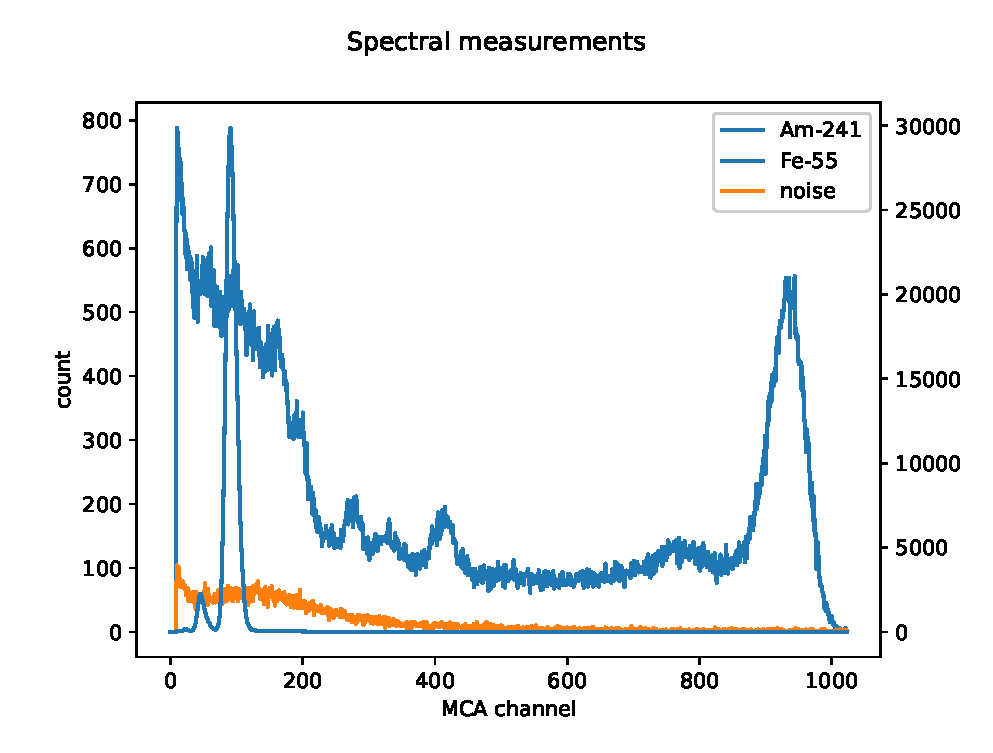
\includegraphics[width=\textwidth]{fig/python/spectra.eps}
\caption{Spectral measurements}
\label{fig:spectra}
\end{figure}

\begin{figure}[ht!]
\centering
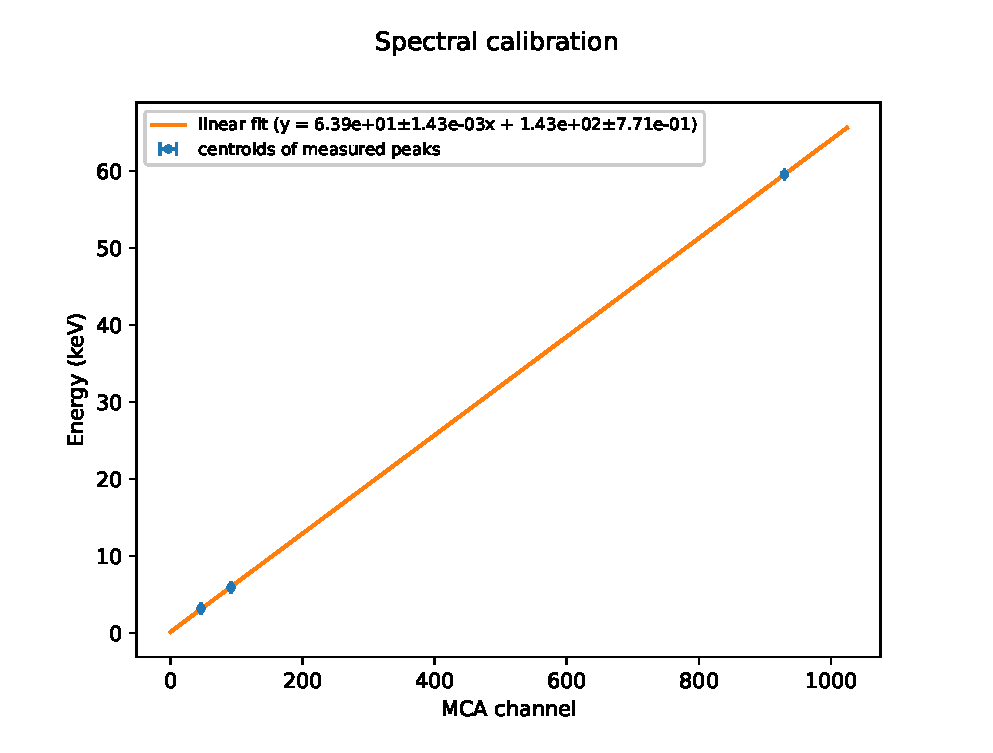
\includegraphics[width=\textwidth]{fig/python/spectral_calibration.eps}
\caption{Energy calibration with the spectral measurement}
\label{fig:spectral_calibration}
\end{figure}



\clearpage
\section{Conclusions}
\label{conclusions}
Discuss results in context.
No need to repeat the results.
Refer to the introduction.
Was the aim fulfilled?
Were the results as expected? If not, why?
Is the mesurement precise enough to discuss ASDF?


\clearpage
\begin{appendices}

\section{Pre-amplifier}
\label{pre_amp}
In addition to using the amplifier available at the lab, we constructed a pre-amplifier ourselves.
This pre-amplifier required a power supply, which we also constructed ourselves, as the operational amplifier used in the pre-amplifier requires supplies of both positive and negative voltage of 5 V.
We started by testing the power supply components on a breadboard, as in figure \ref{fig:pre_amp_psu_testing}.
Once we had verified that the components worked, we soldered them on a PCB, resulting in the device in figure \ref{fig:pre_amp_psu}

Figure \ref{fig:pre_amp_schematic} provides a schematic of this pre-amplifier.
Its core is the
\href{https://www.ti.com/product/OPA657}{Texas Instruments OPA657}
\href{https://en.wikipedia.org/wiki/Operational_amplifier}{operational amplifier}, which is configured for the gain value $G = 21$ with a suitable choice of resistors.

TODO GAIN FORMULA HERE

The assembled pre-amplifier is shown in figure \ref{fig:pre_amp_board}, and its mounting is illustrated in figure \ref{fig:pre_amp_mounting}.
We also built a switch panel of figure \ref{fig:pre_amp_switch} for the power supply.
The final assembled pre-amplifier is shown in figure \ref{fig:pre_amp}.

\begin{todo}
Describe preamp construction and what was planned to do with it
\end{todo}

\begin{figure}[ht!]
\centering
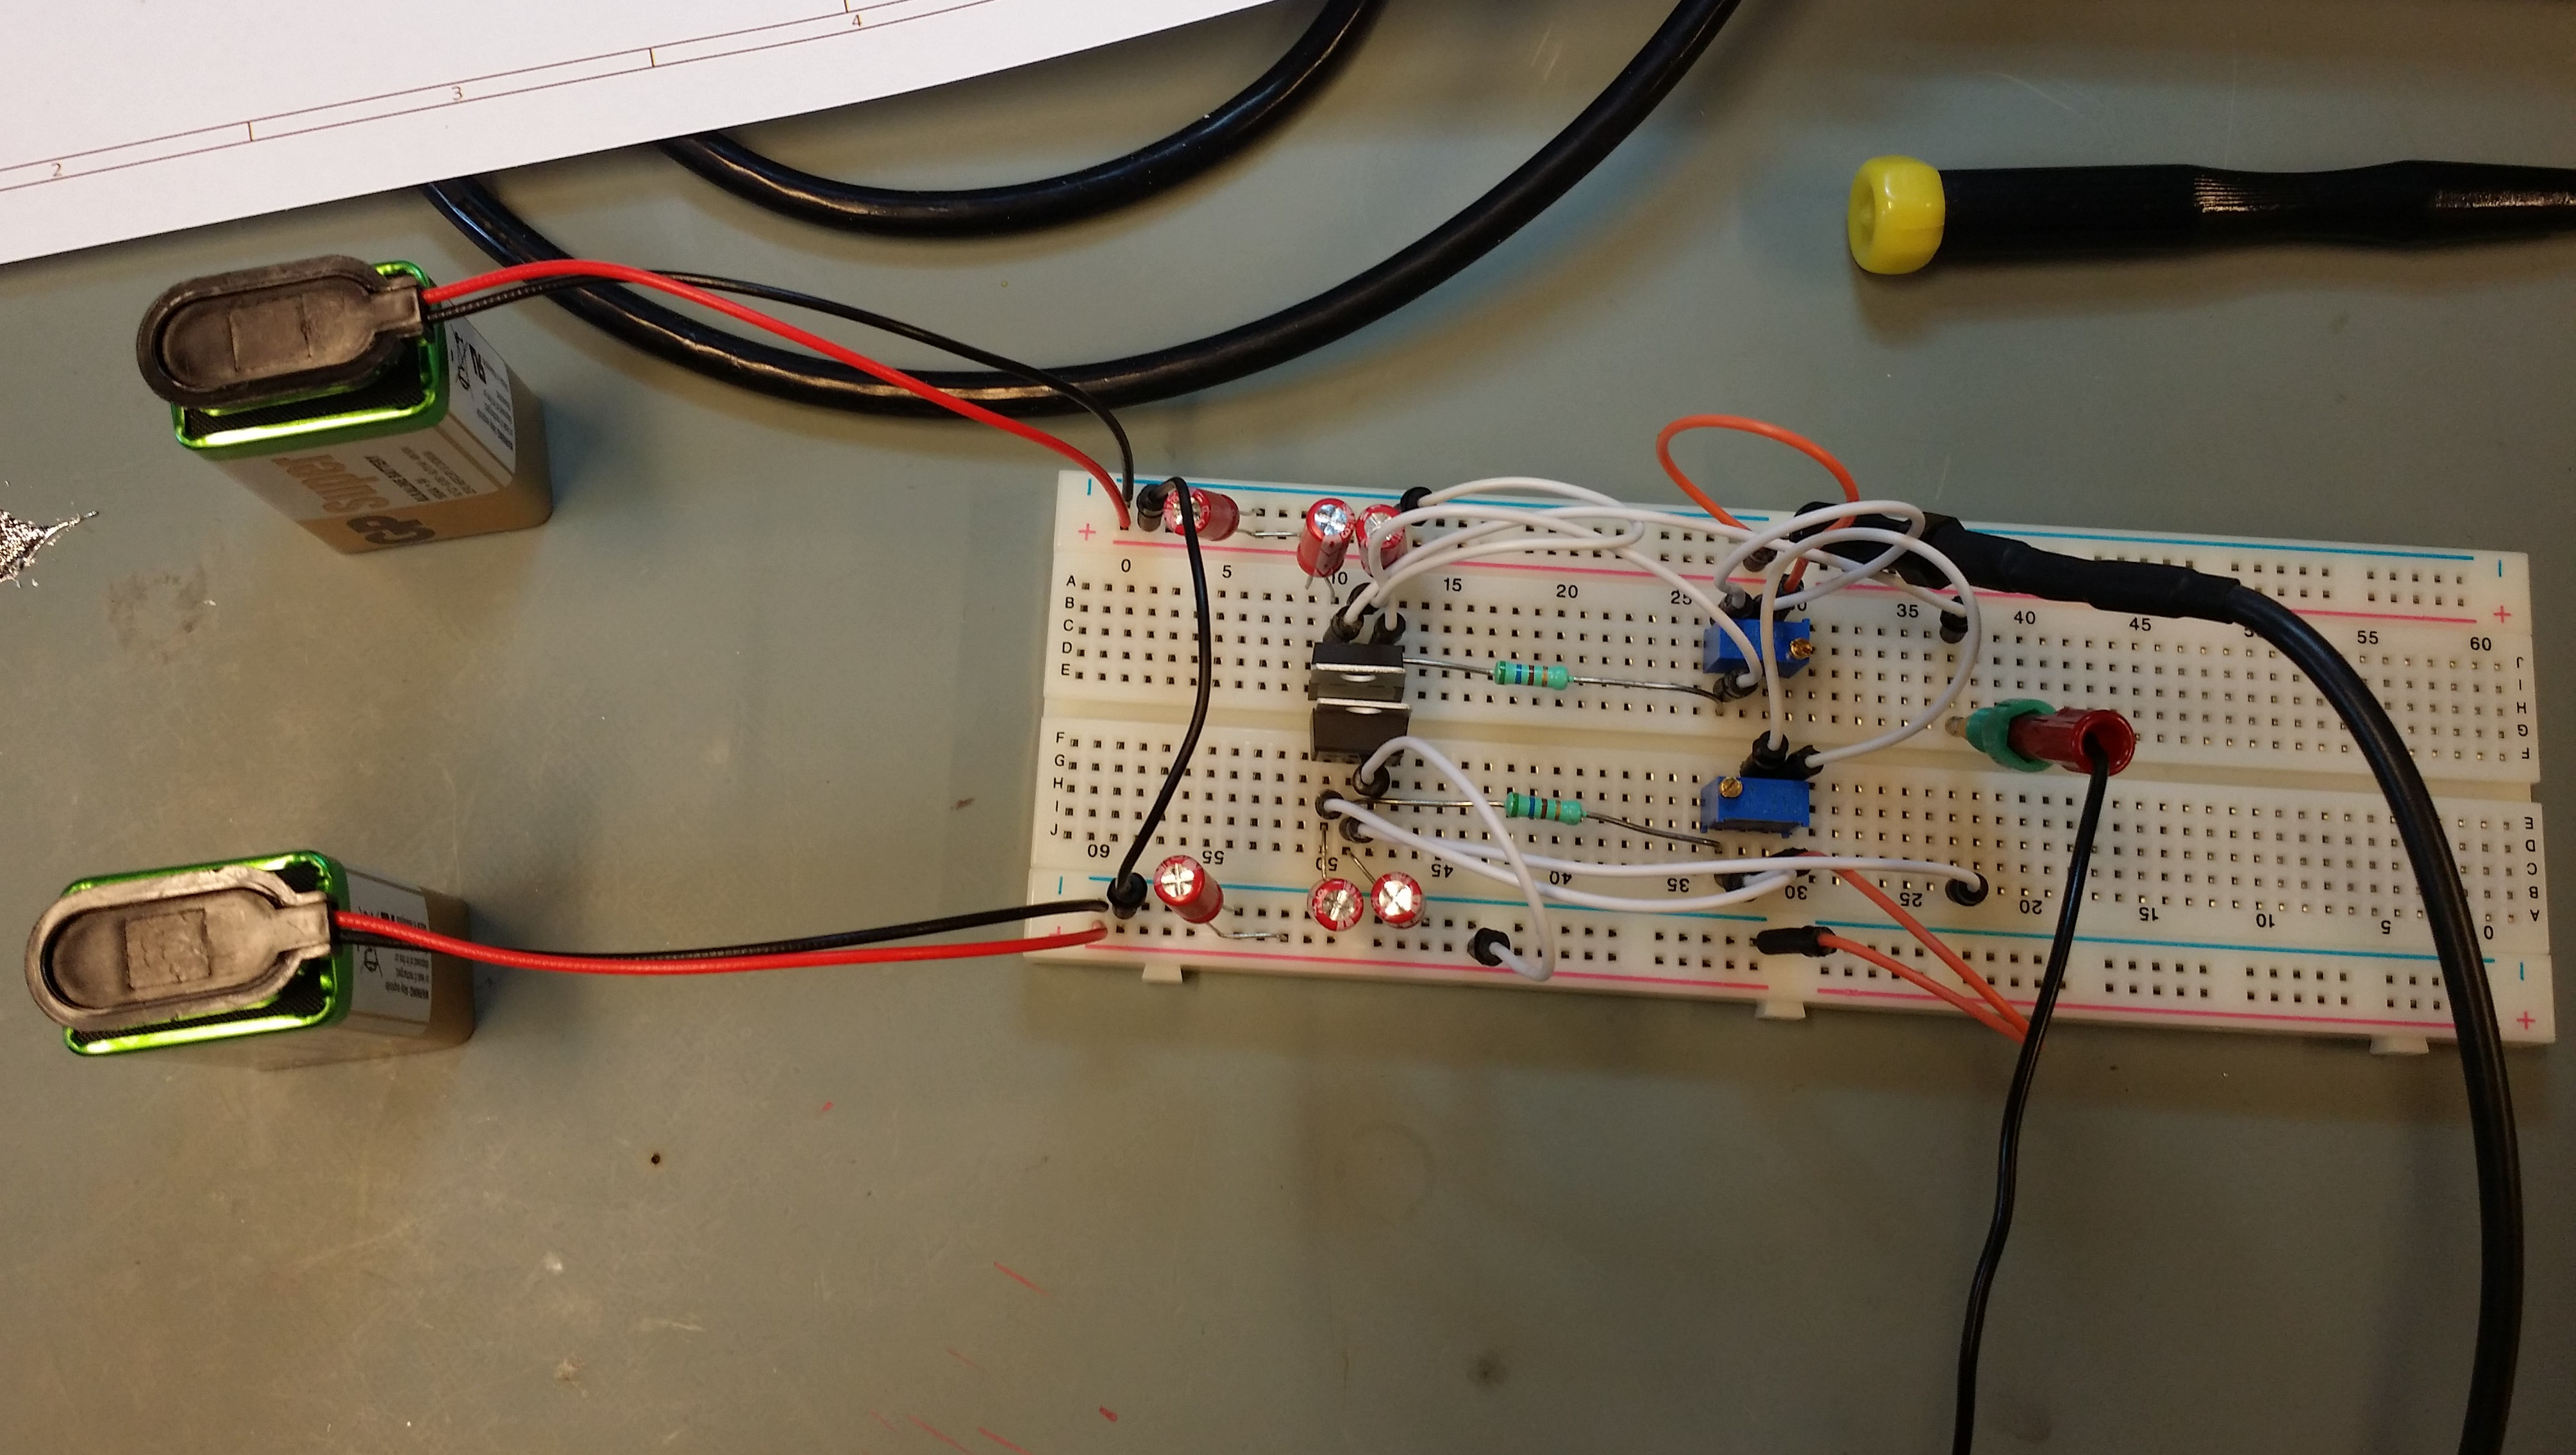
\includegraphics[width=\textwidth]{fig/IMG_20201005_104331-cropped.jpg}
\caption{Preliminary testing of the components of the pre-amplifier power supply}
\label{fig:pre_amp_psu_testing}
\end{figure}

\begin{figure}[ht!]
\centering

\begin{subfigure}[t]{0.48\textwidth}
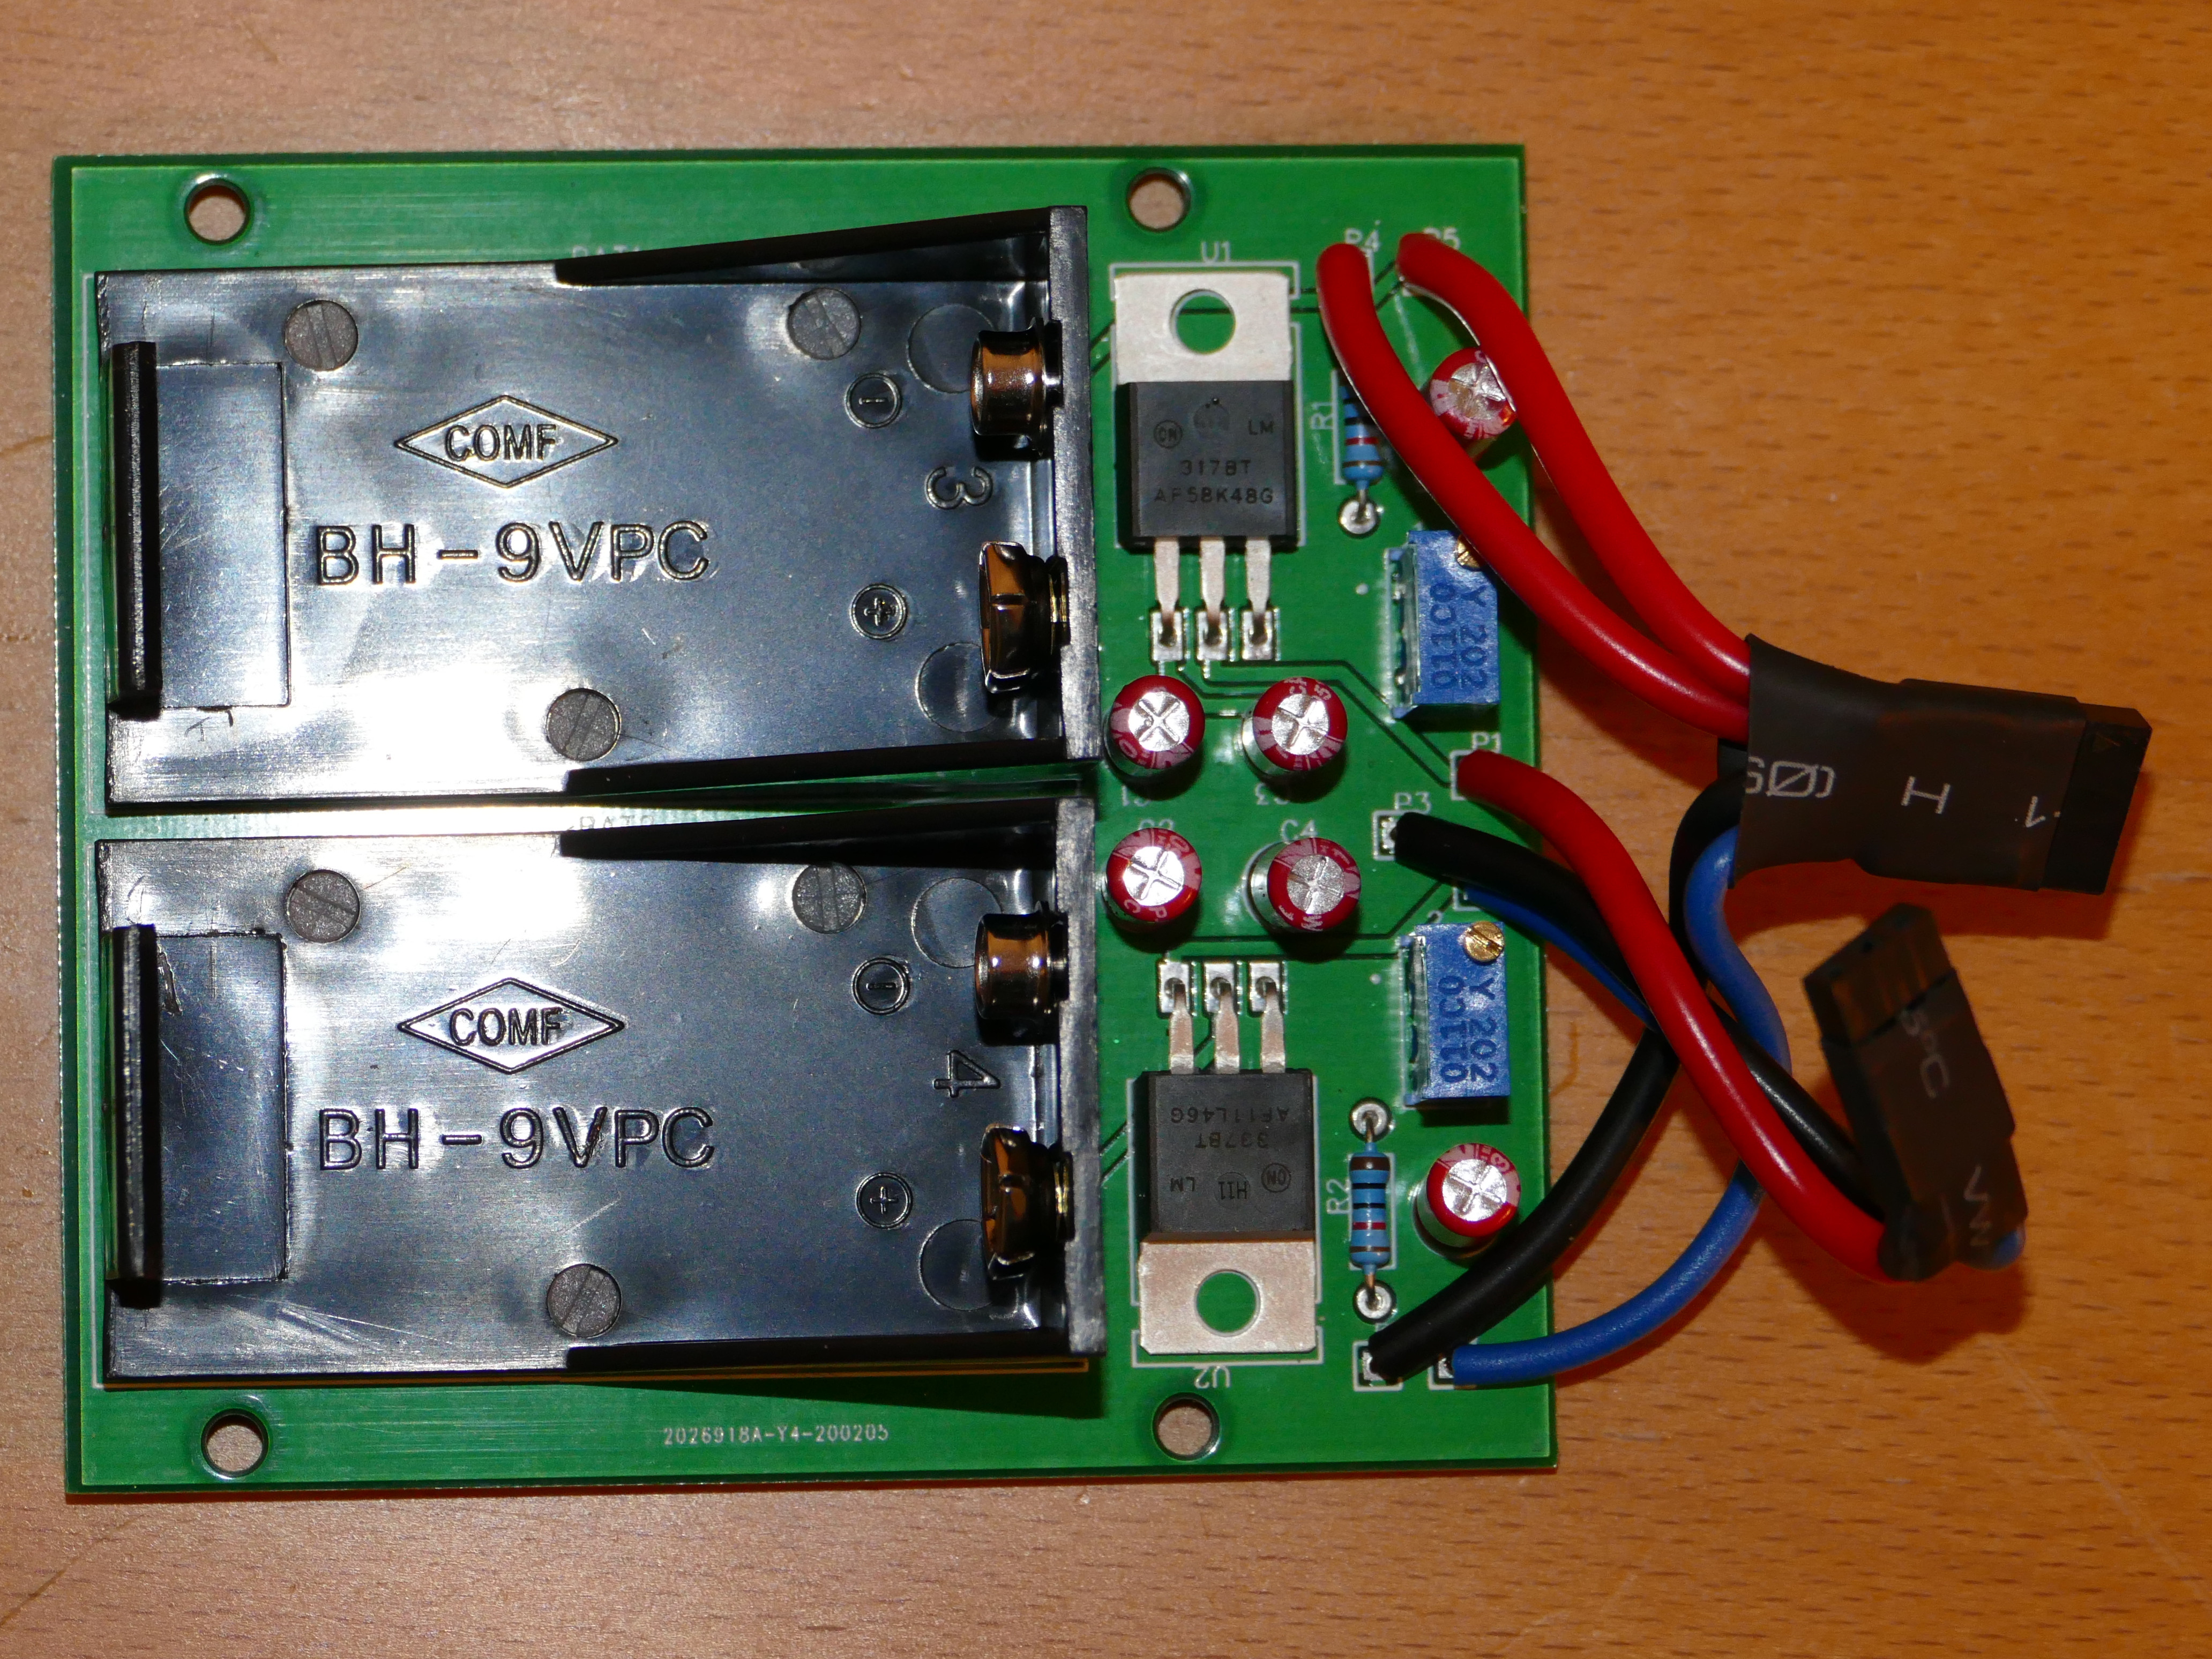
\includegraphics[width=\textwidth]{fig/P1170891-cropped.jpg}
\end{subfigure}
%
\begin{subfigure}[t]{0.48\textwidth}
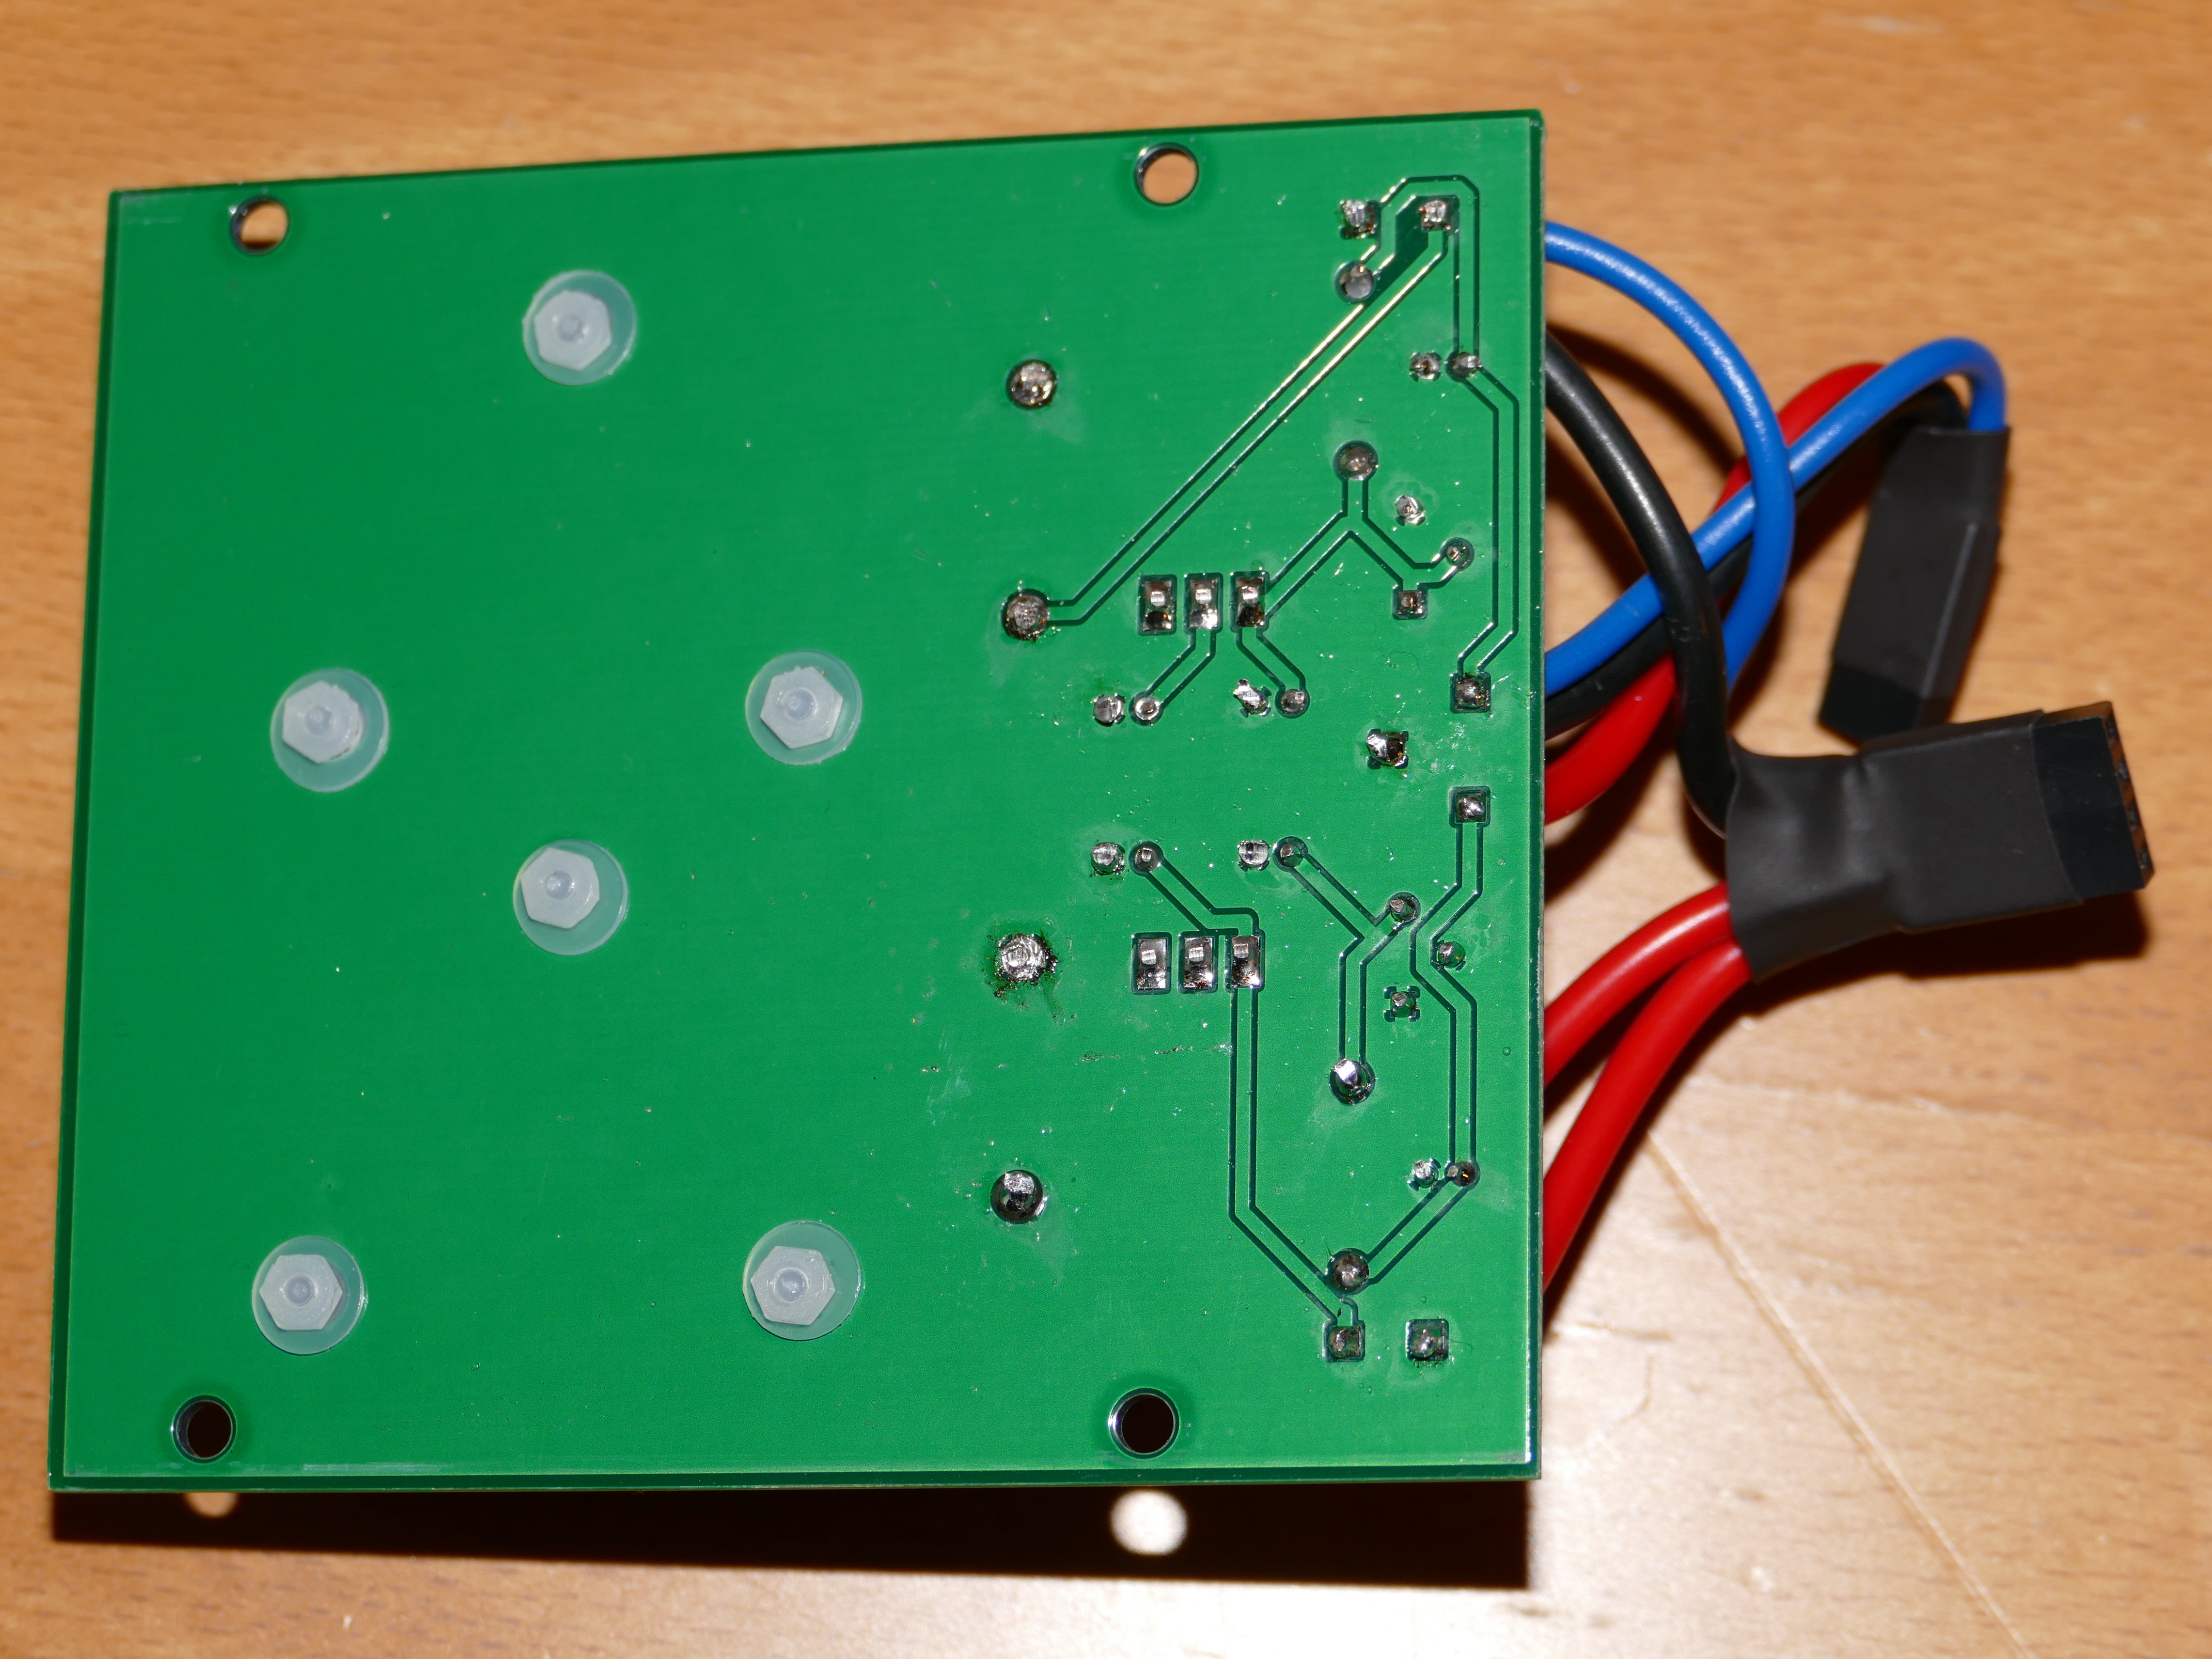
\includegraphics[width=\textwidth]{fig/P1170894-cropped.jpg}
\end{subfigure}
%
\caption{Power supply for the pre-amplifier}
\label{fig:pre_amp_psu}
\end{figure}

\begin{figure}[ht!]
\centering
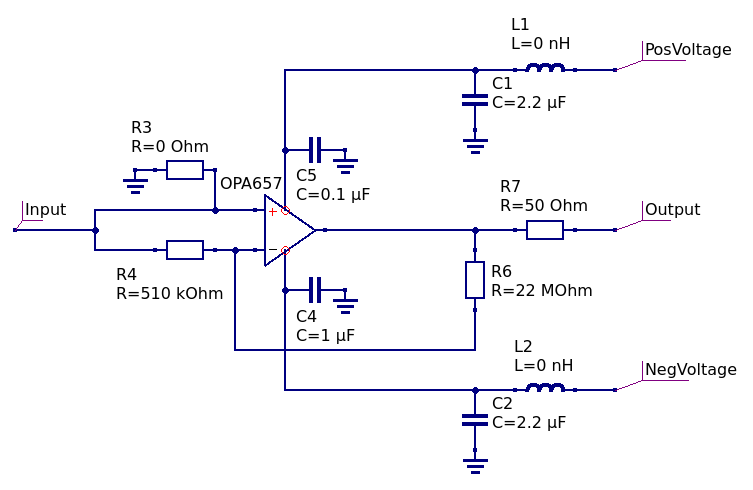
\includegraphics[width=\textwidth]{fig/amp-schematic/amplifier.png}
\caption{Circuit diagram of the pre-amplifier}
\label{fig:pre_amp_schematic}
\end{figure}

\begin{figure}[ht!]
\centering
% 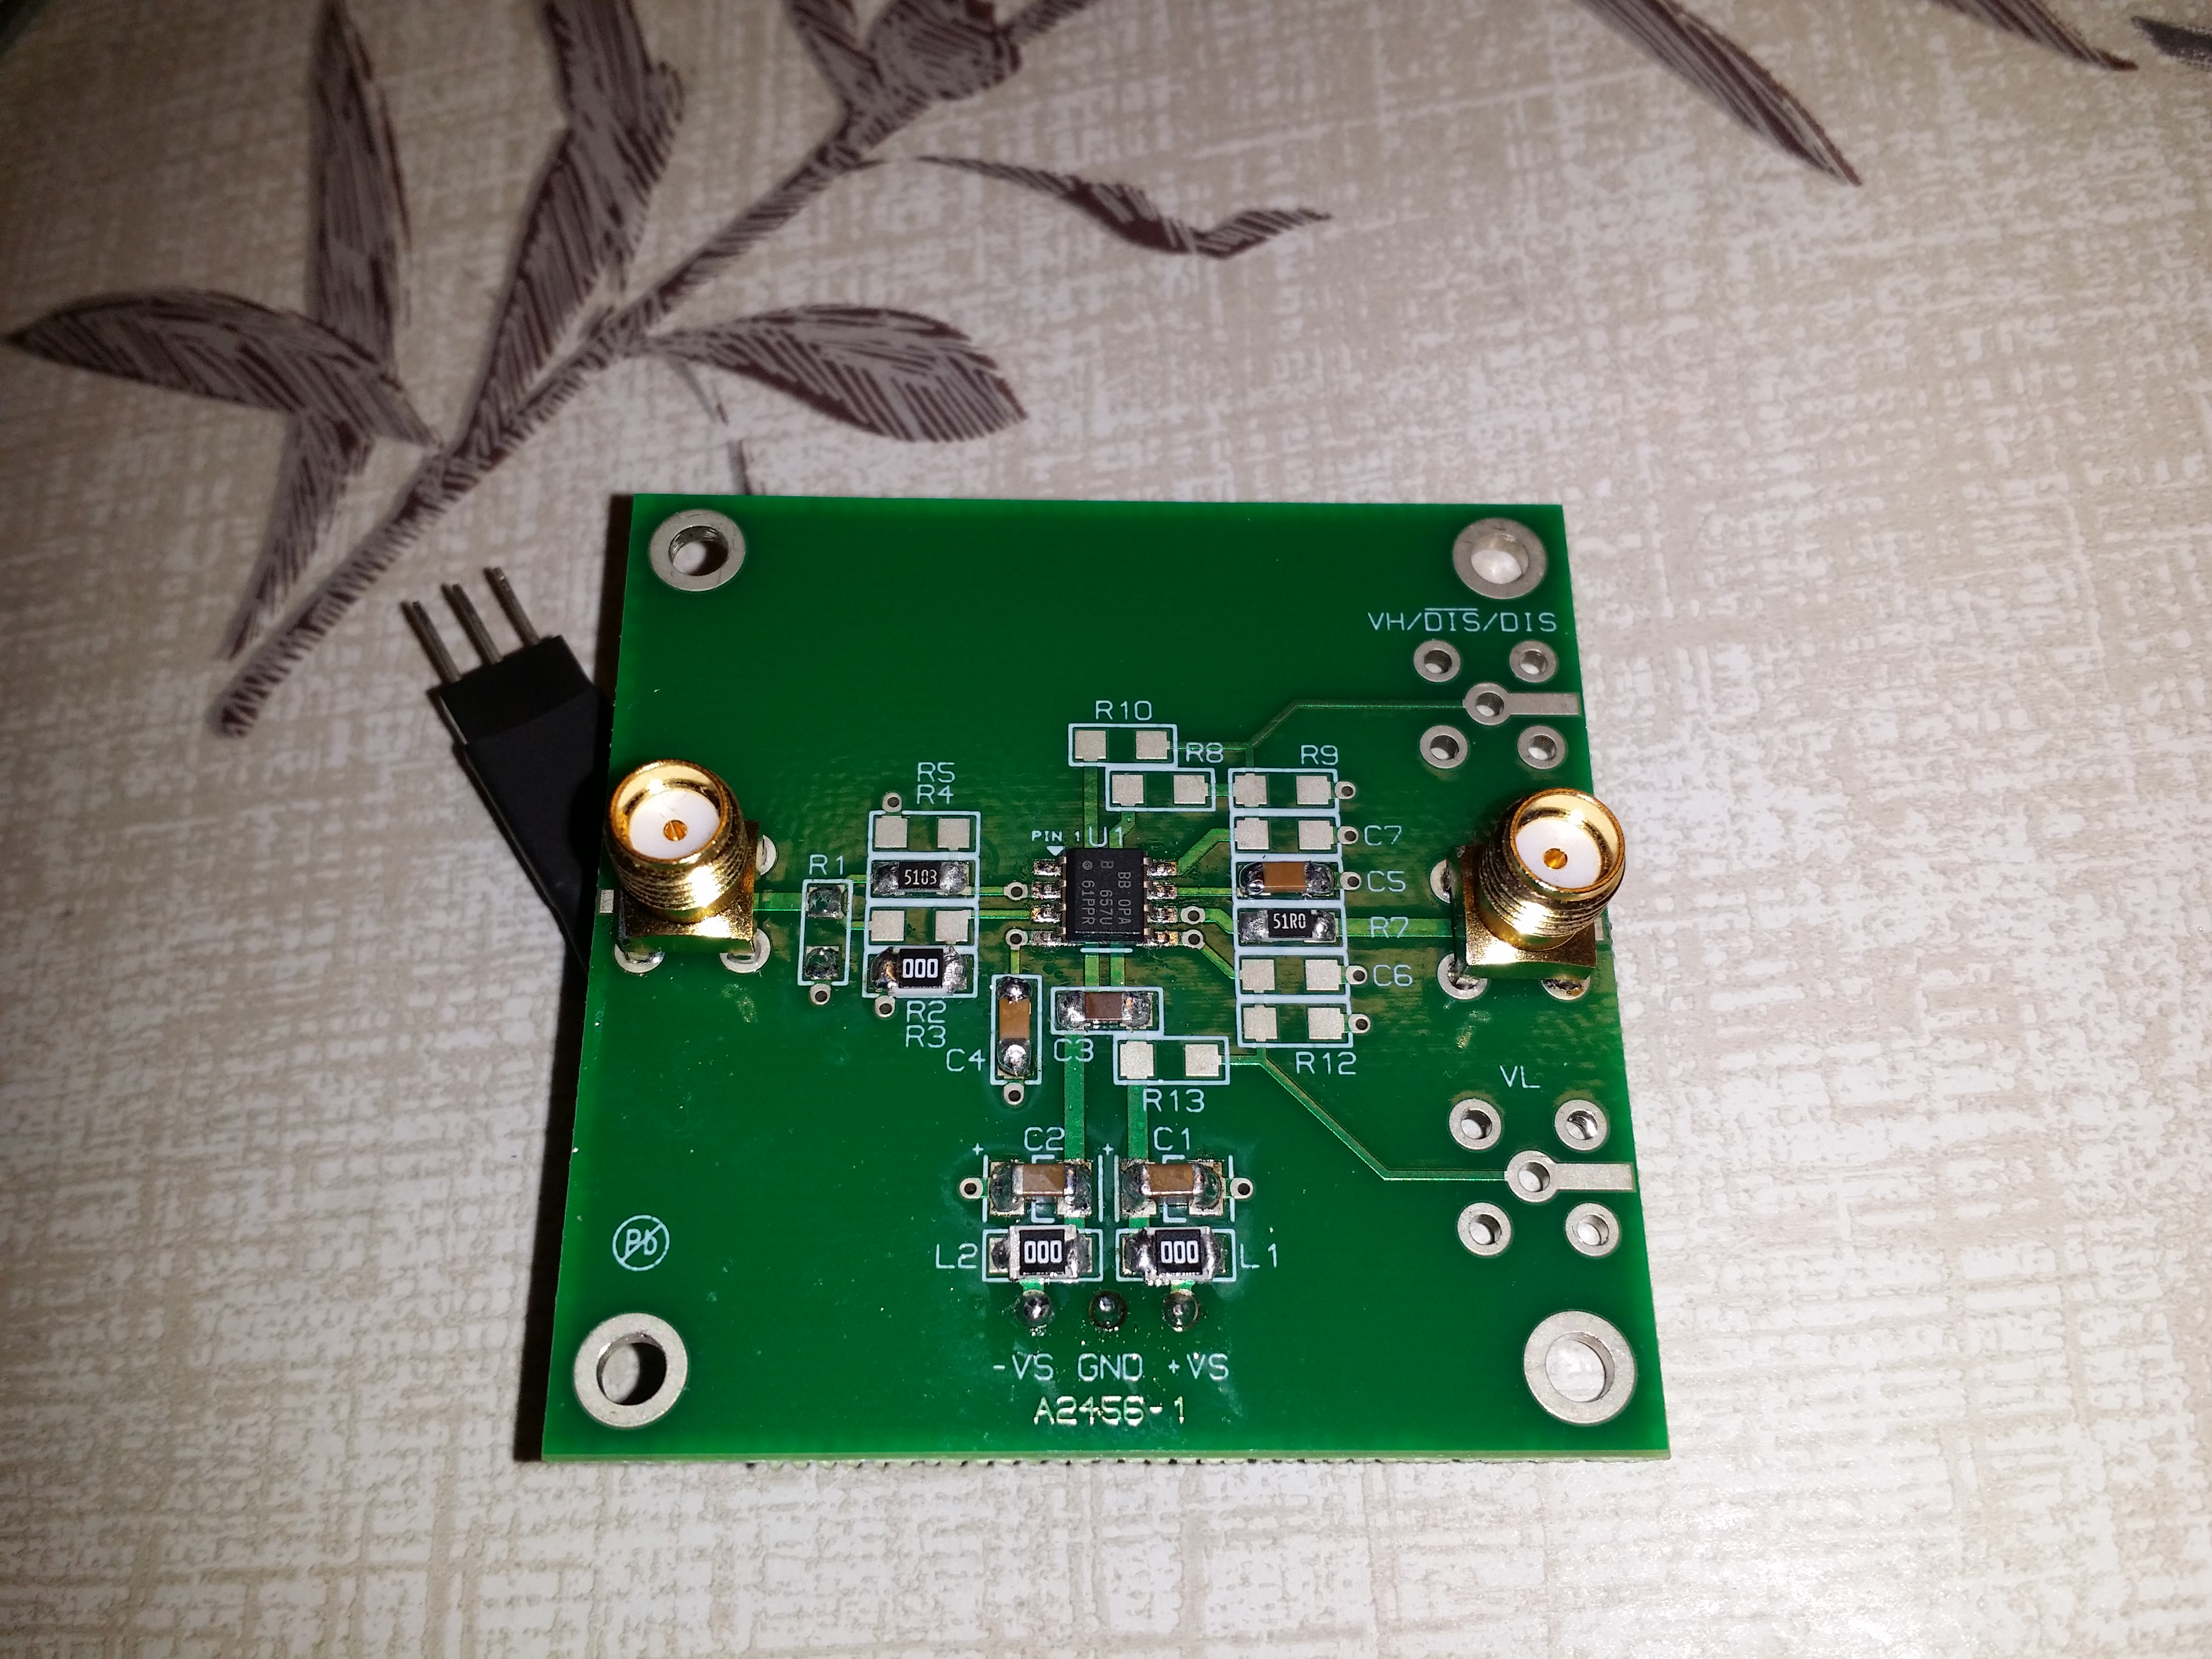
\includegraphics[width=\textwidth]{fig/IMG_20201207_121010.jpg}
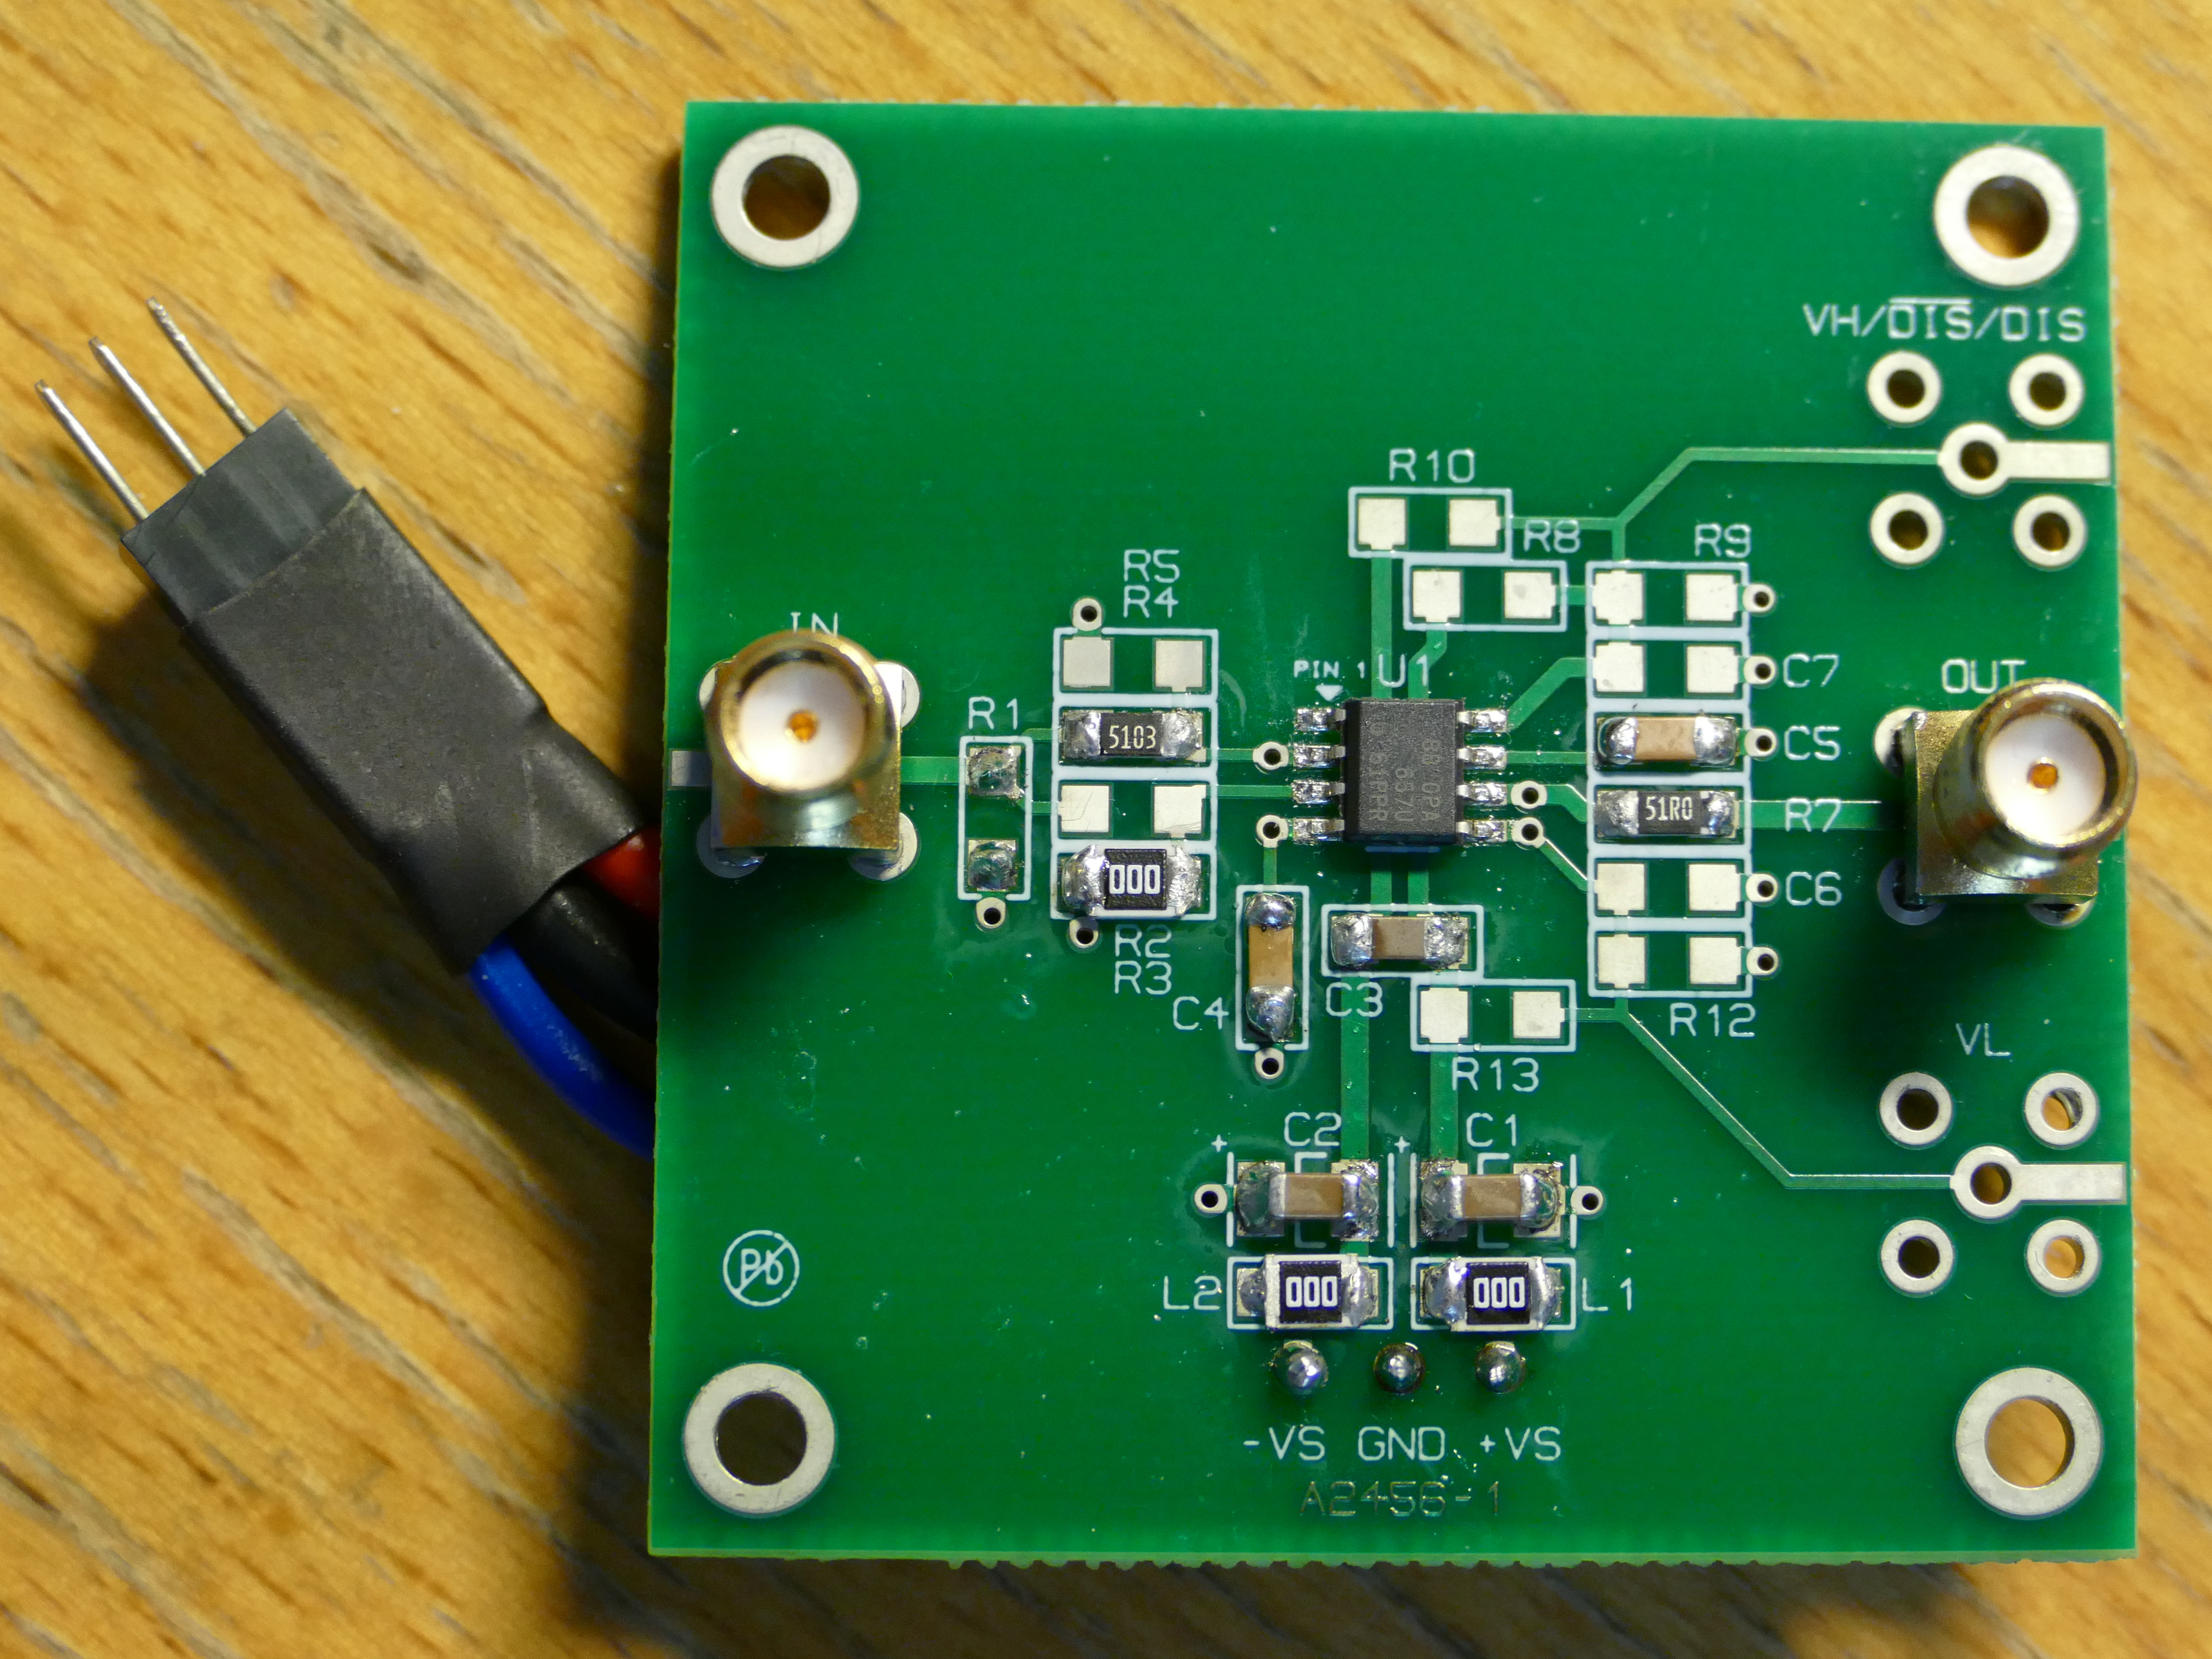
\includegraphics[width=0.9\textwidth]{fig/P1170917-cropped.jpg}
\caption{Pre-amplifier board}
\label{fig:pre_amp_board}
\end{figure}

\begin{figure}[ht!]
\centering
\begin{subfigure}[t]{0.48\textwidth}
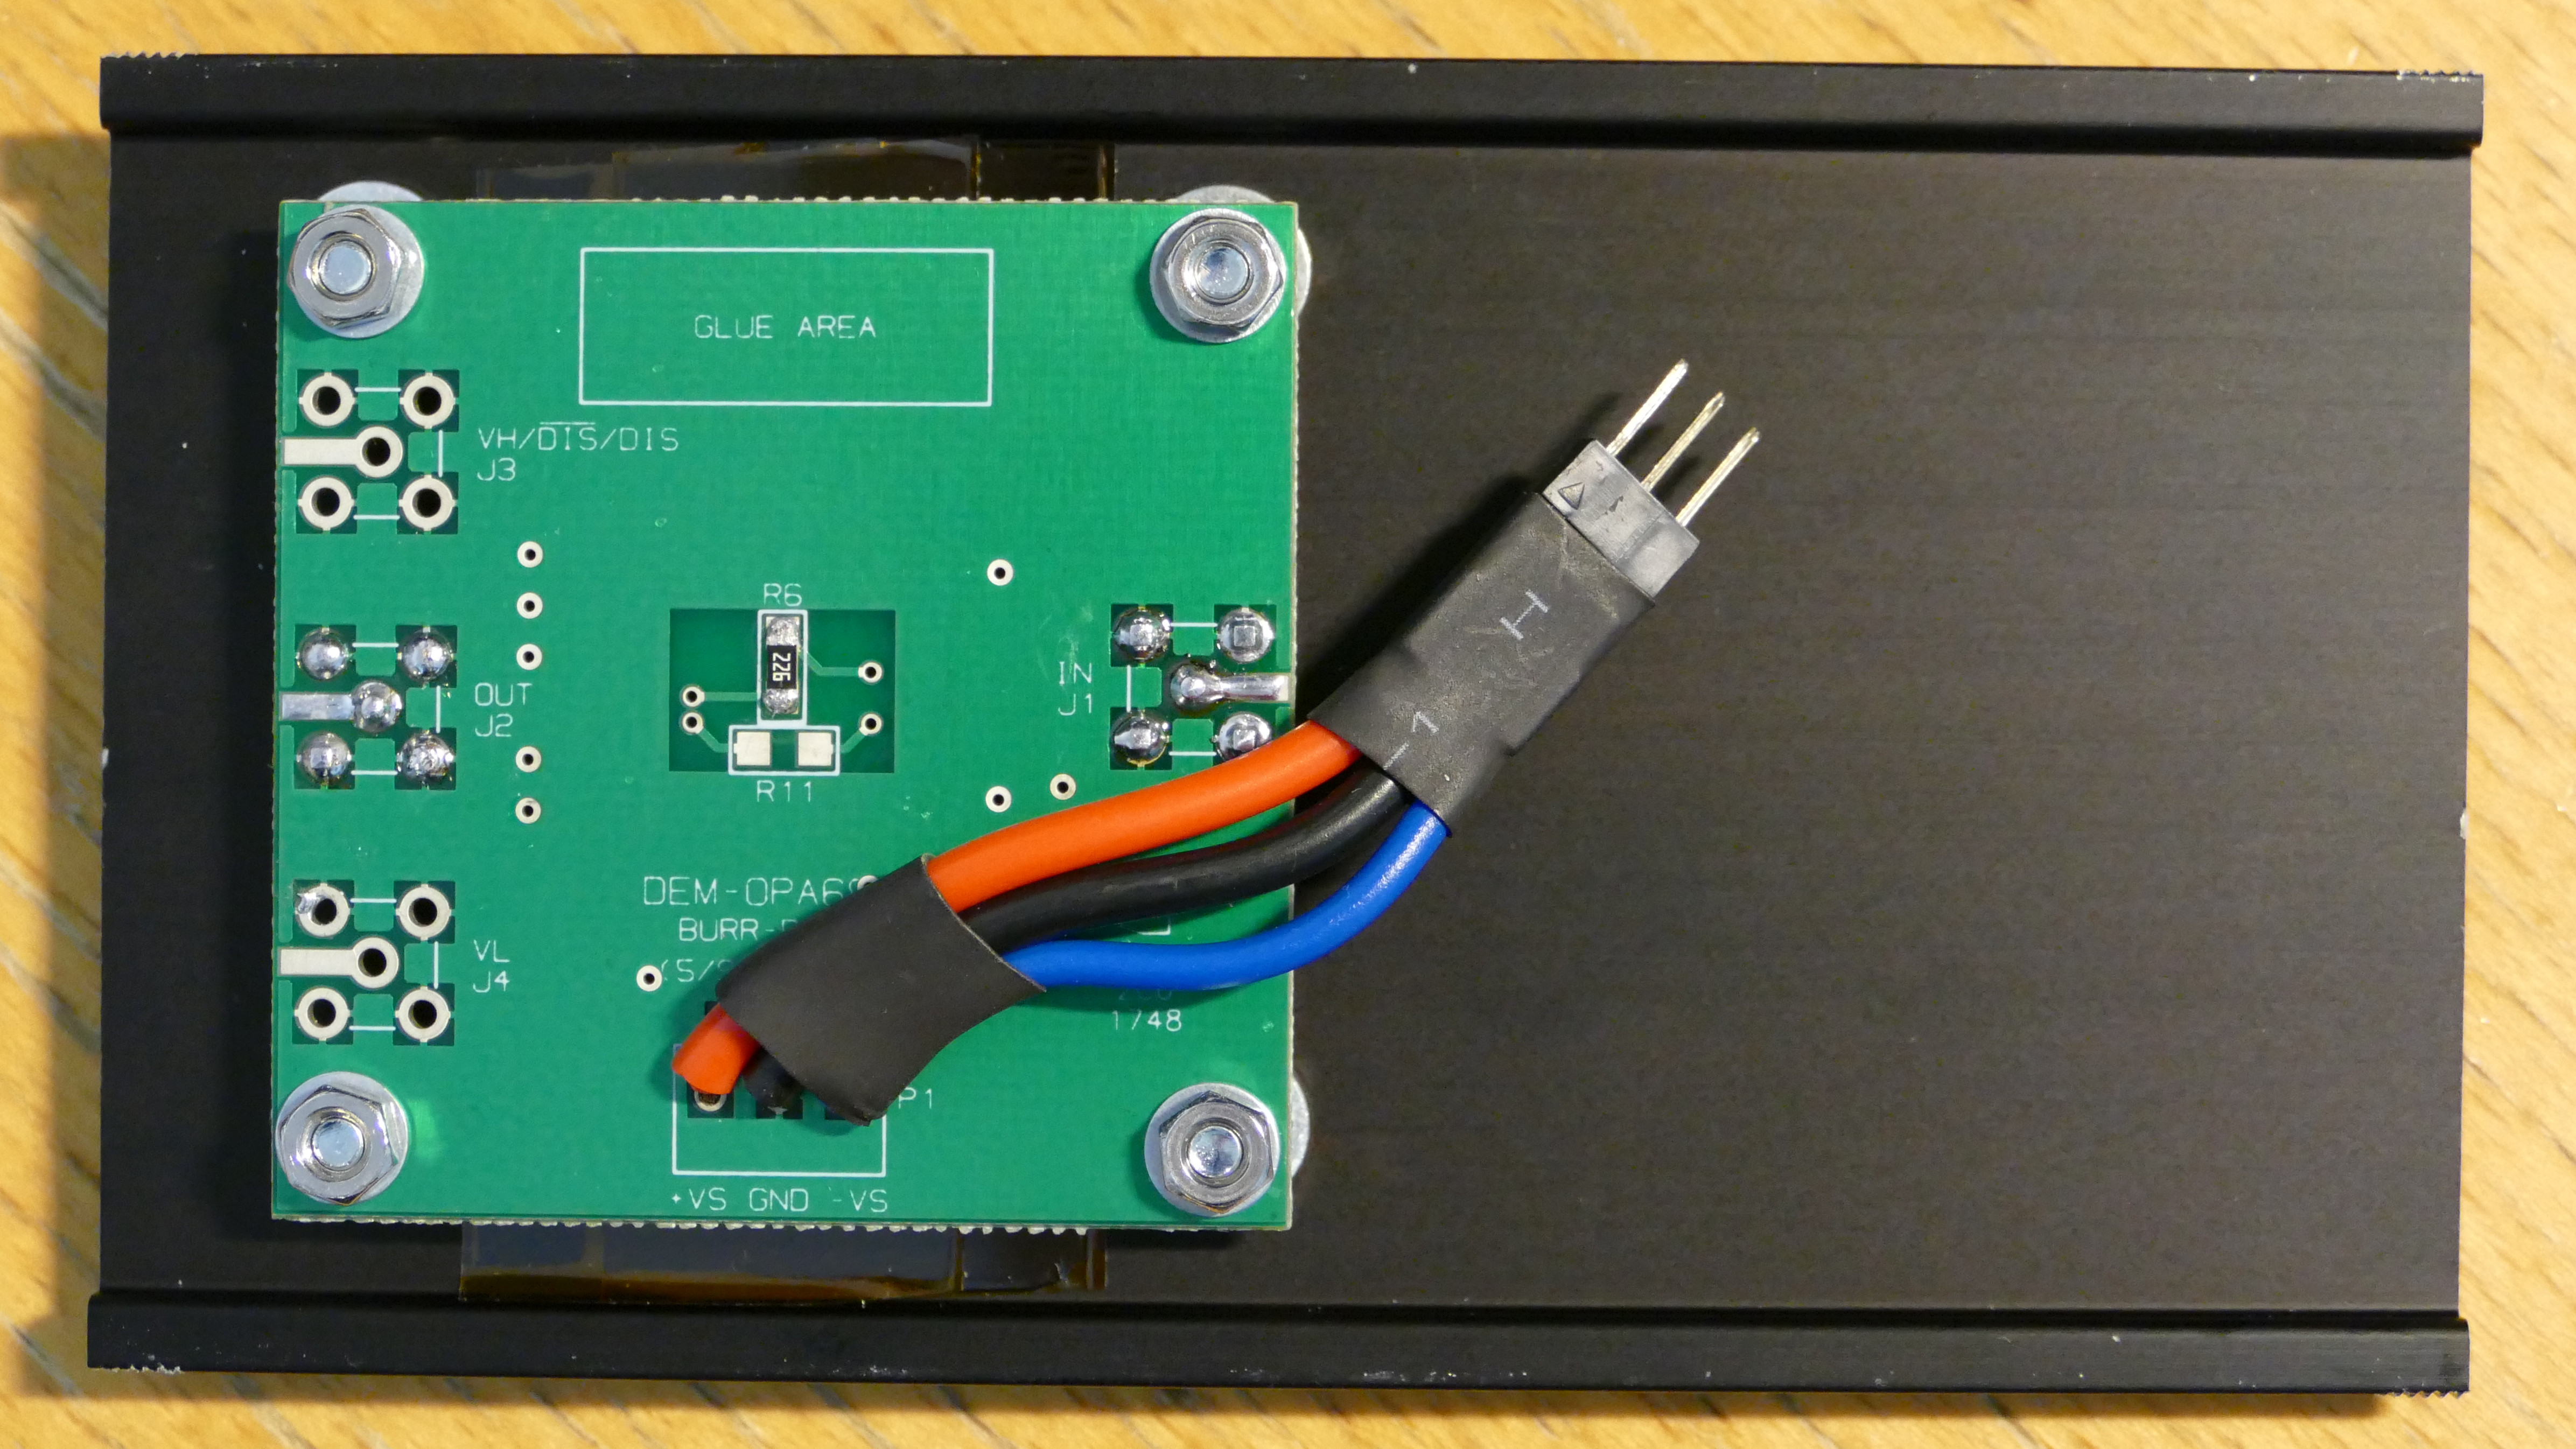
\includegraphics[width=\textwidth]{fig/P1170915-cropped.jpg}
\end{subfigure}
%
\begin{subfigure}[t]{0.48\textwidth}
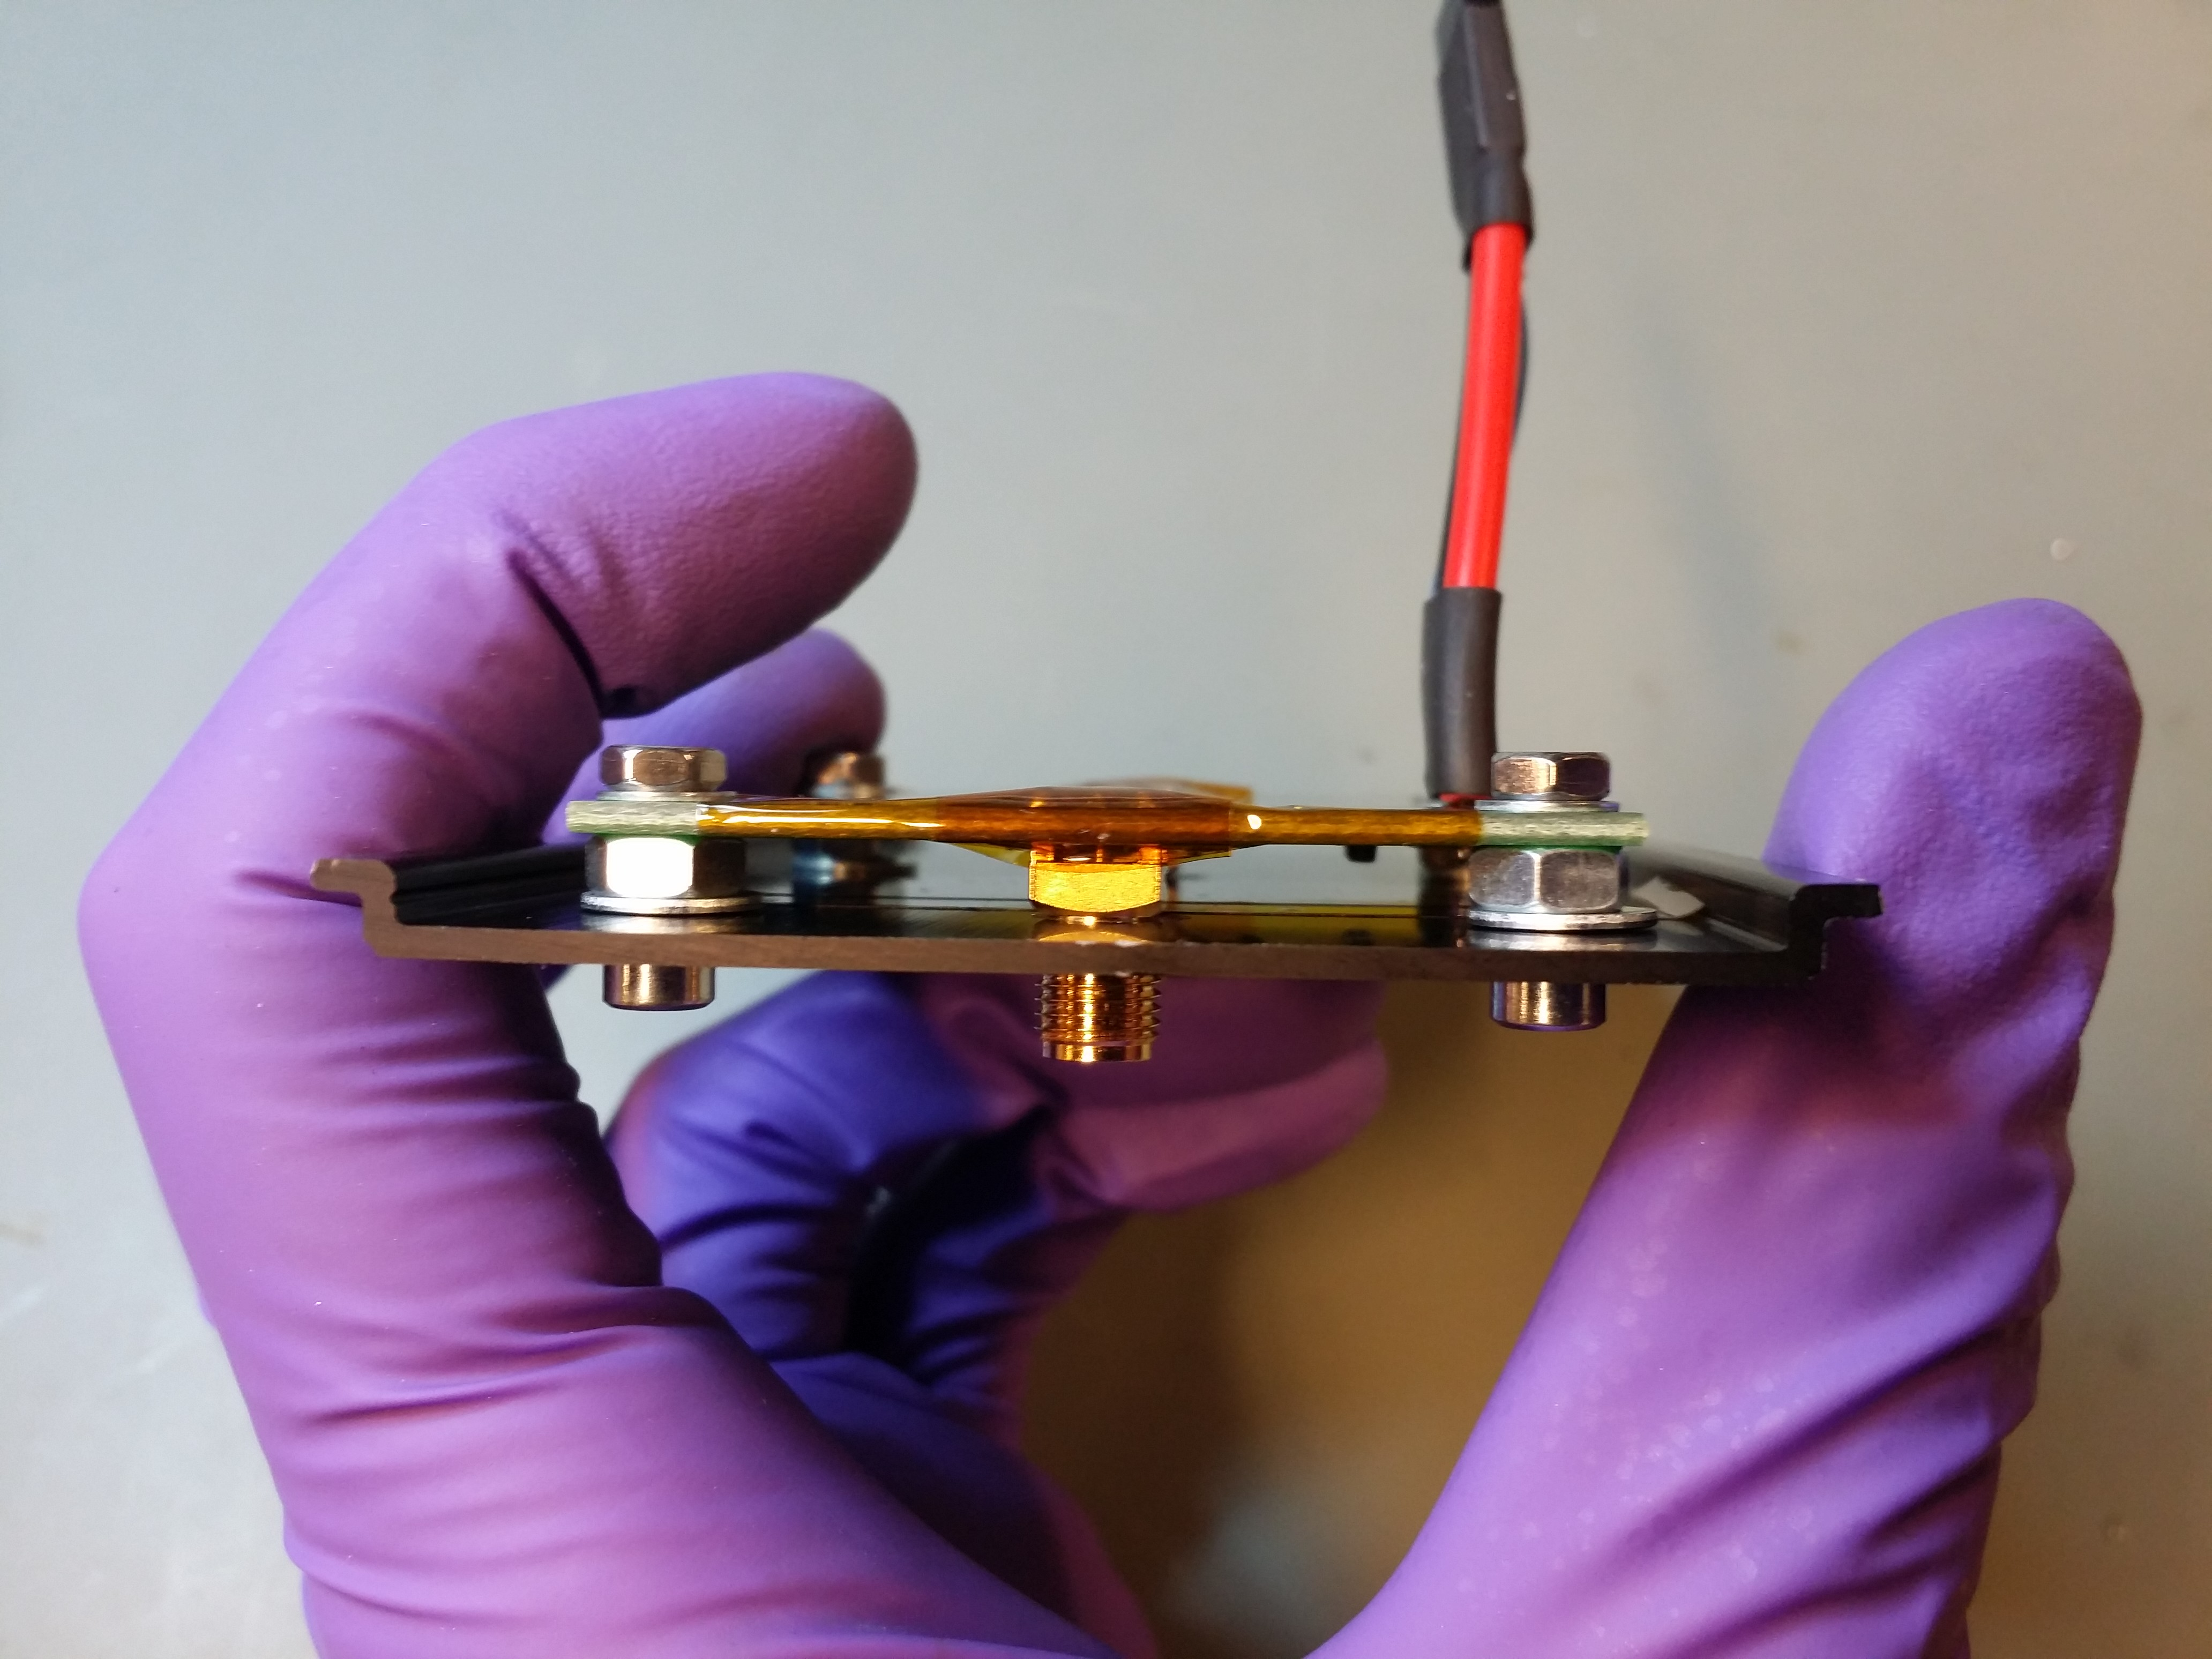
\includegraphics[width=\textwidth]{fig/IMG_20201201_121845.jpg}
\end{subfigure}

\begin{subfigure}[t]{0.48\textwidth}
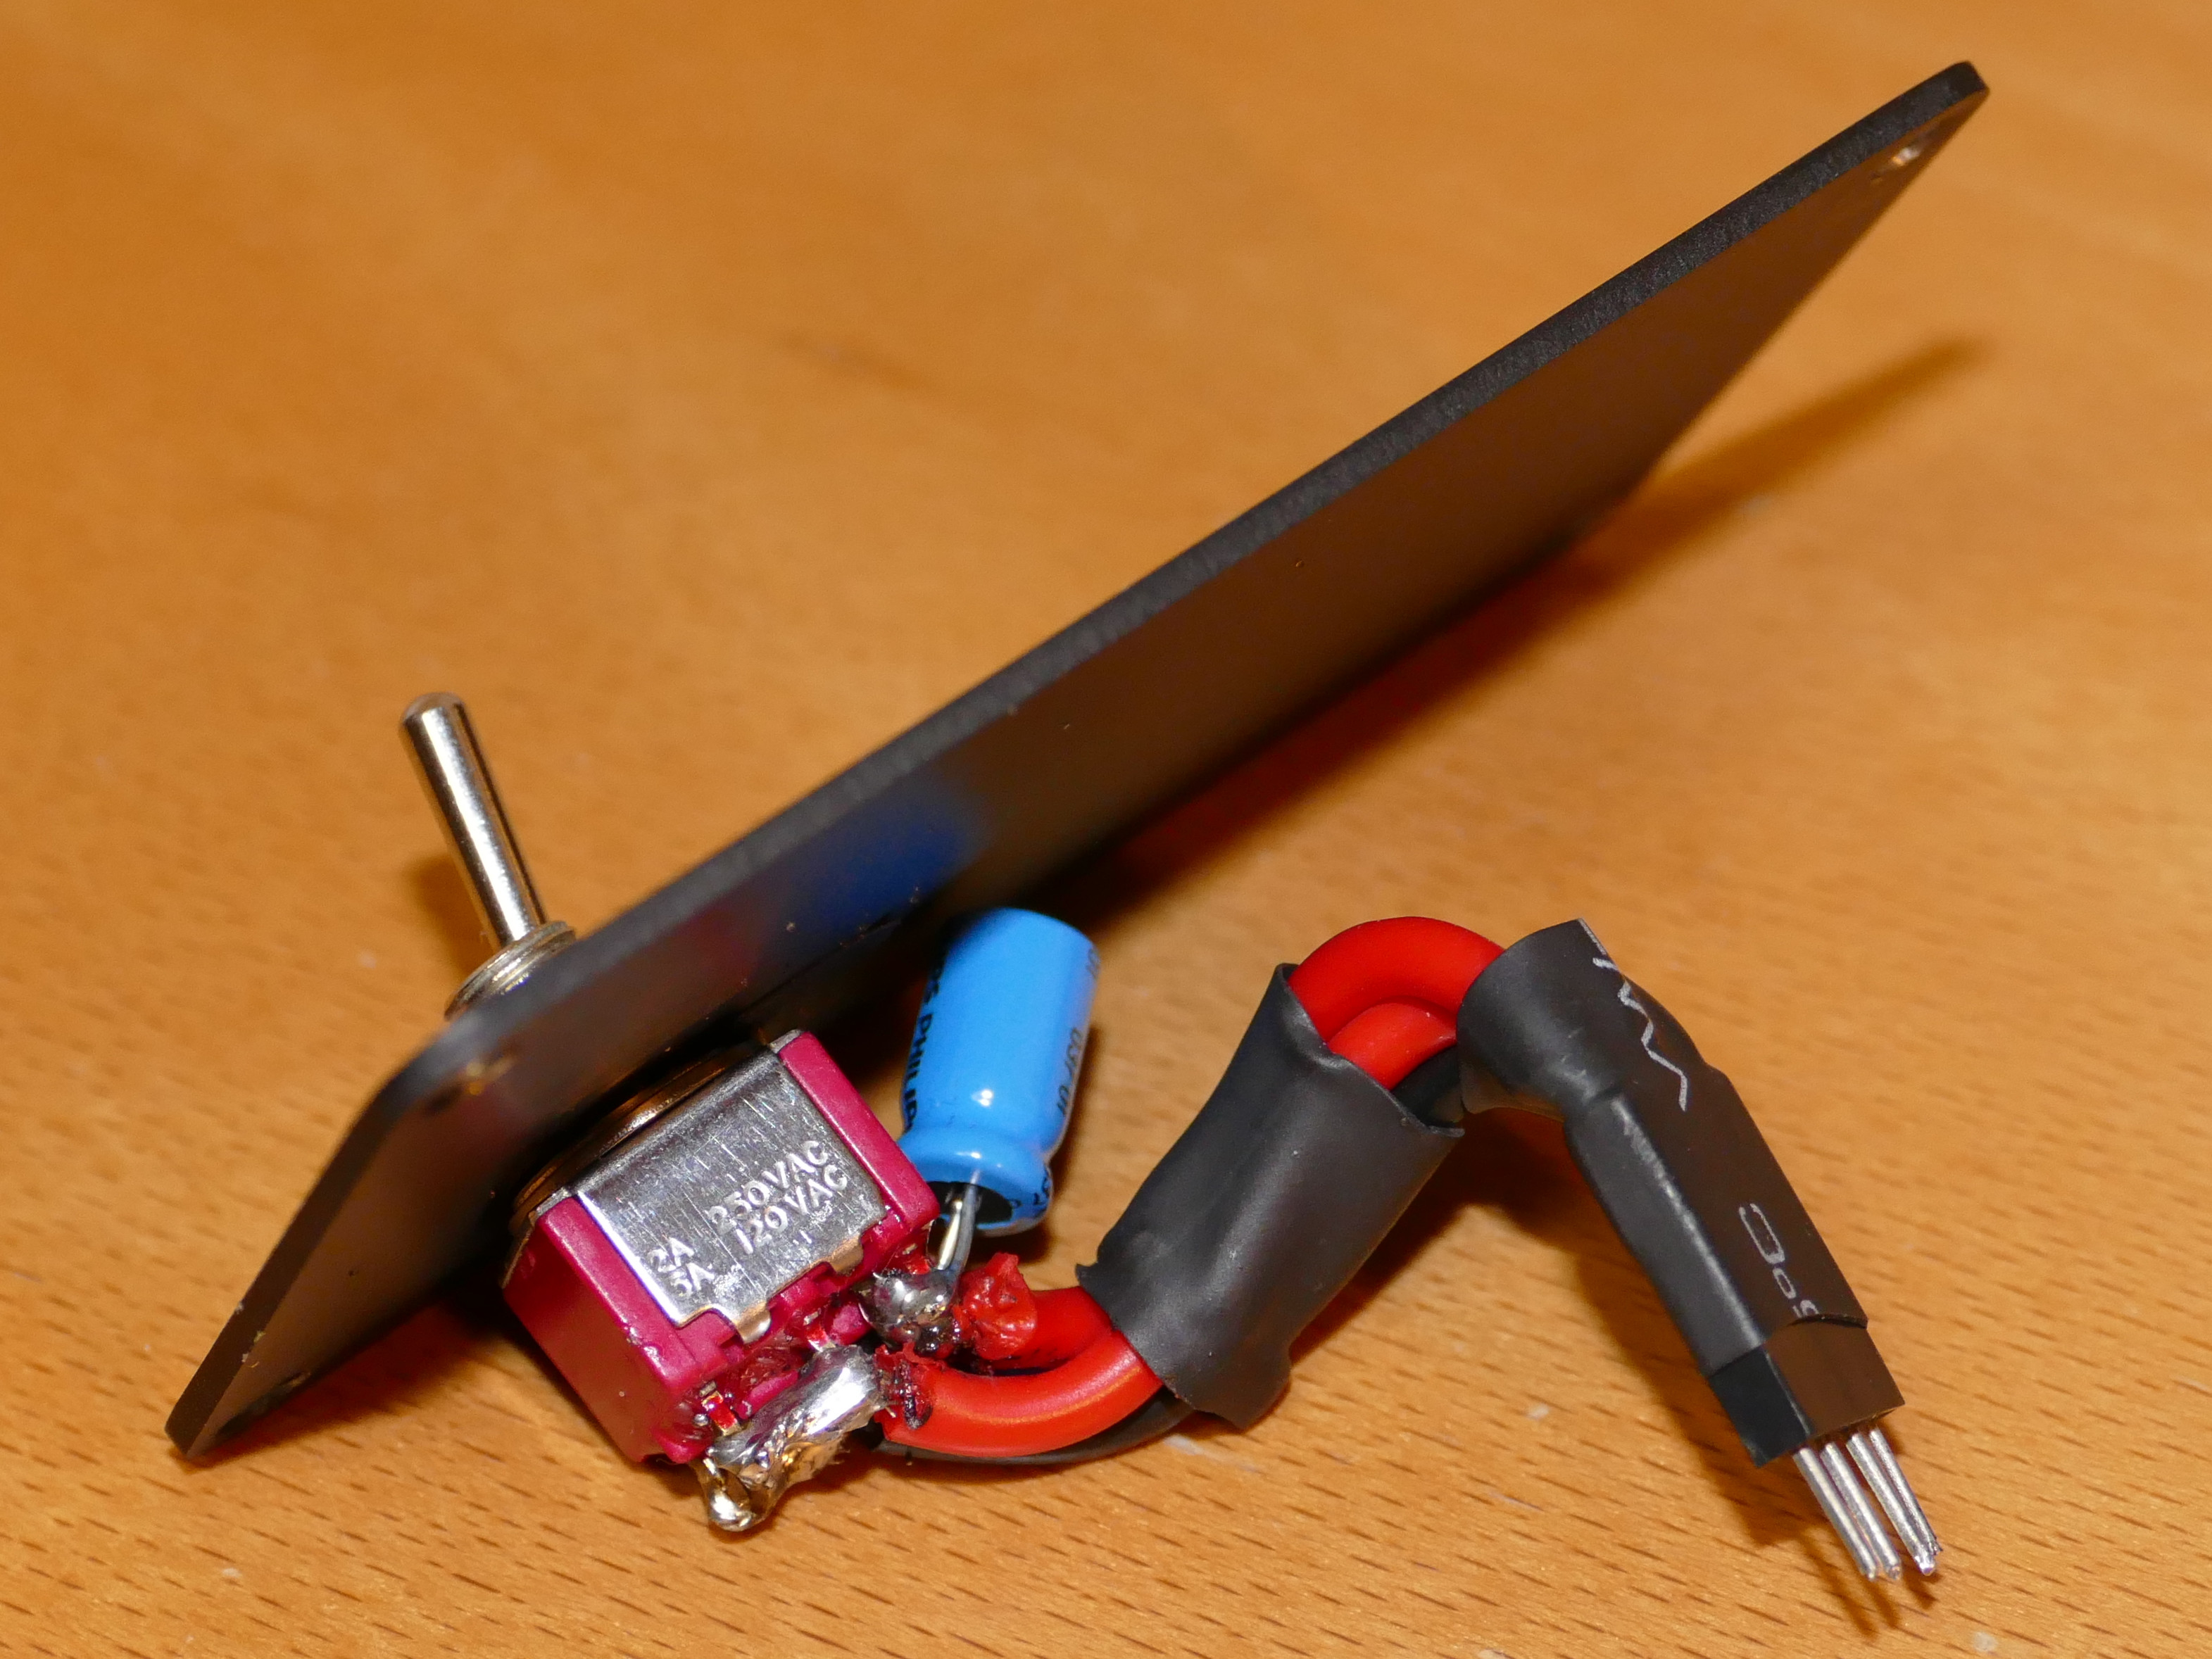
\includegraphics[width=\textwidth]{fig/P1170907-cropped.jpg}
\caption{Pre-amplifier switch panel}
\label{fig:pre_amp_switch}
\end{subfigure}
%
\begin{subfigure}[t]{0.48\textwidth}
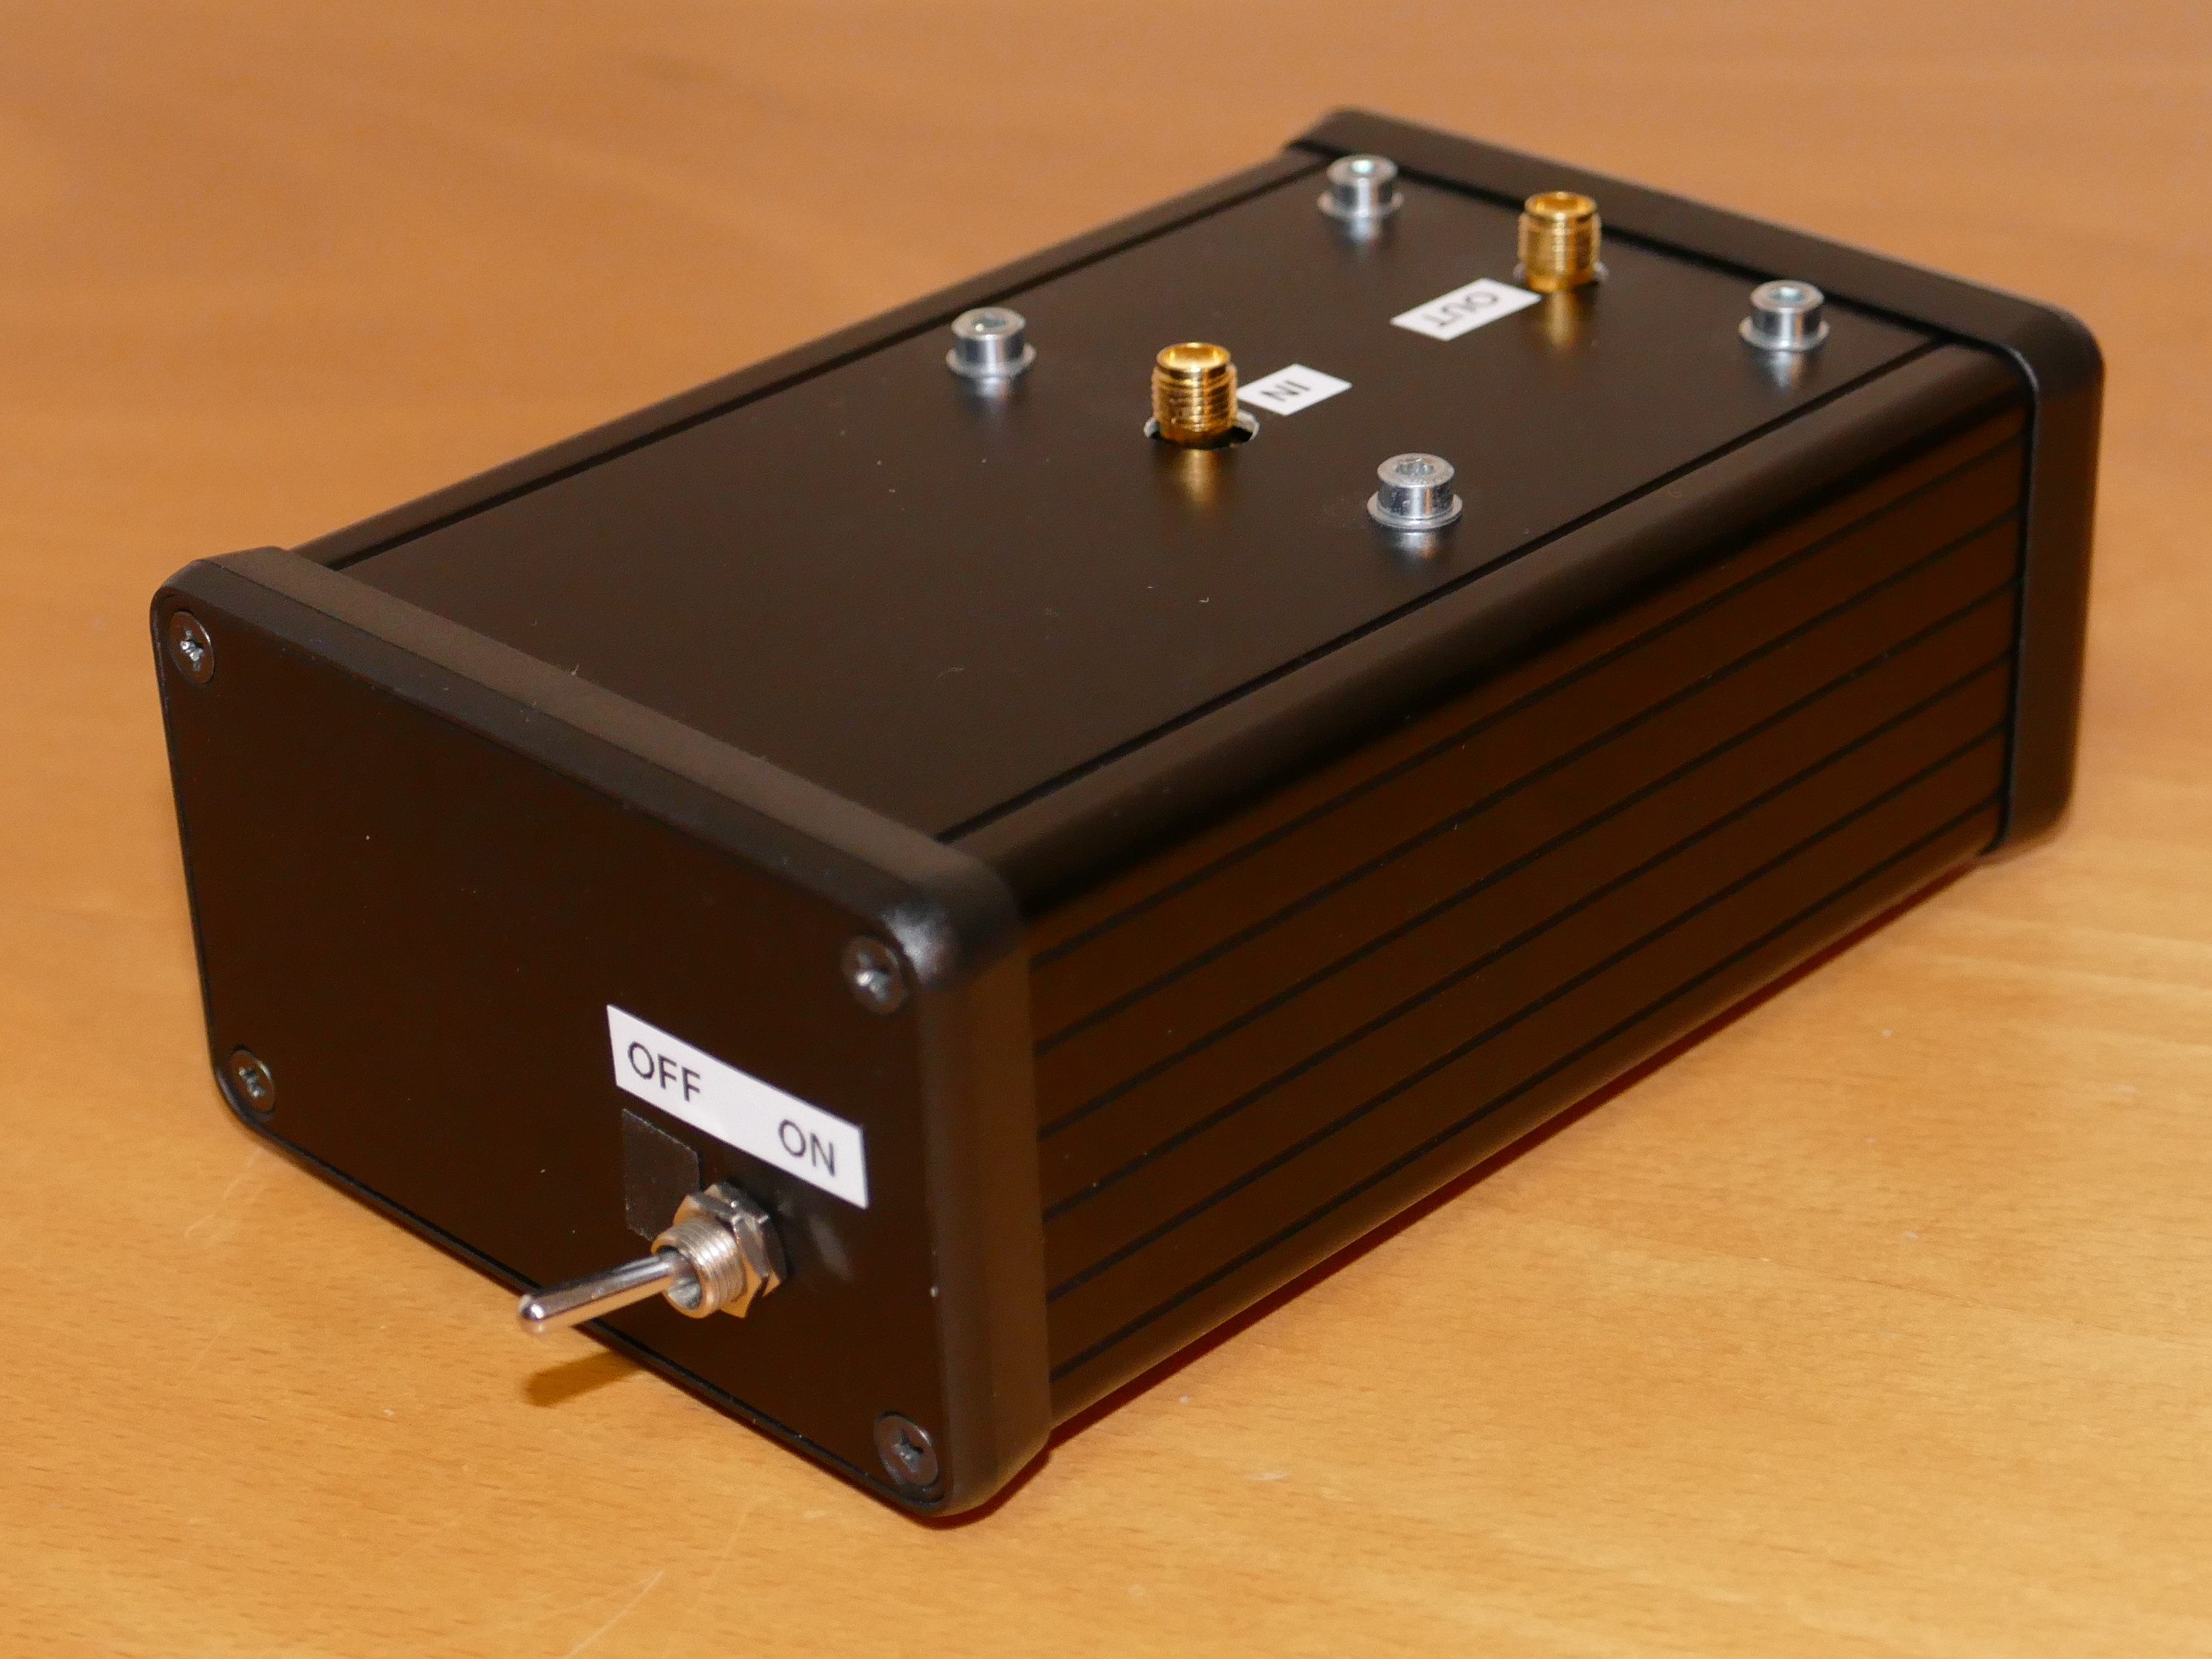
\includegraphics[width=\textwidth]{fig/P1170874-cropped.jpg}
\caption{Pre-amplifier}
\label{fig:pre_amp}
\end{subfigure}
%
\caption{Pre-amplifier case and mounting}
\label{fig:pre_amp_mounting}
\end{figure}


\clearpage
Once the pre-amplifier was assembled, we tested its frequency response with an external pulser.
These results are plotted in figure \ref{fig:pre_amp_freq_response}.
The frequency reponse is flat up to 10 kHz, but then fluctuates significantly, as the reflections of the signal within the amplifier become significant.

\begin{figure}[ht!]
\centering
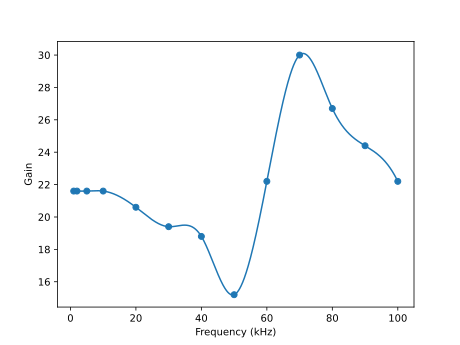
\includegraphics[width=\textwidth]{fig/python/preamp_freq_response}
\caption{Frequency response of the pre-amplifier}
\label{fig:pre_amp_freq_response}
\end{figure}


\begin{figure}[ht!]
\centering
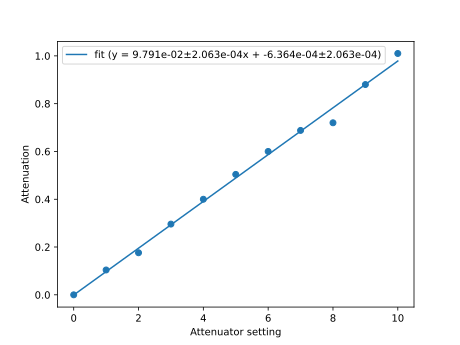
\includegraphics[width=\textwidth]{fig/python/attenuator}
\caption{Attenuator calibration at $f$ = 10 kHz}
\label{fig:attenuator}
\end{figure}

\begin{figure}[ht!]
\centering
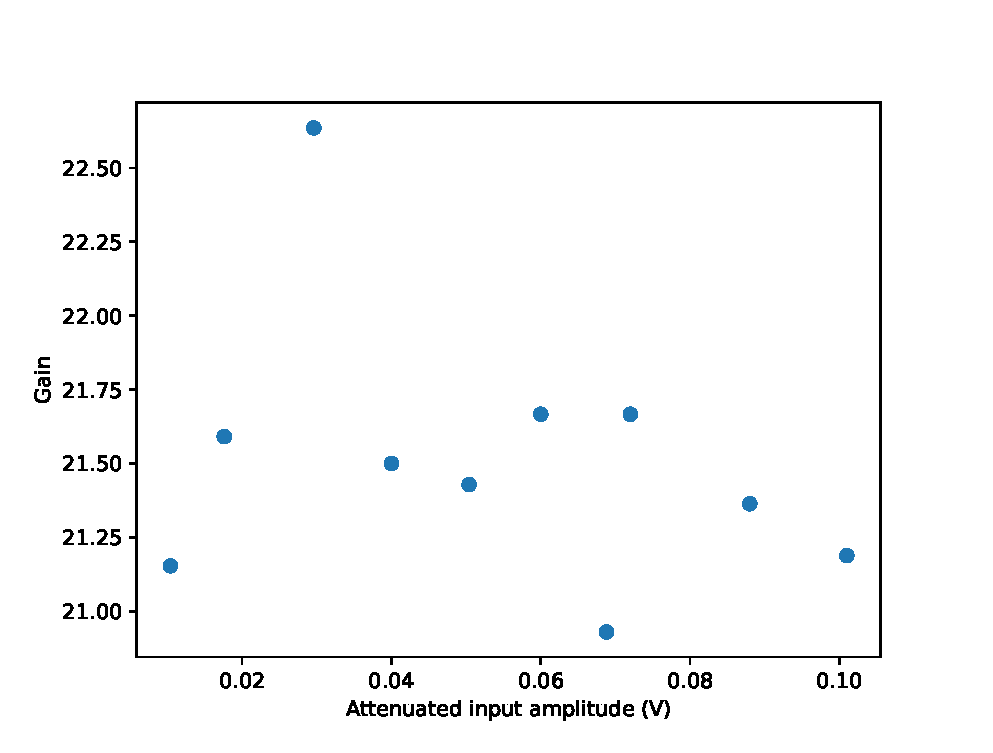
\includegraphics[width=\textwidth]{fig/python/preamp_gain}
\caption{Pre-amplifier gain by input amplitude at $f$ = 10 kHz}
\label{fig:attenuator}
\end{figure}


\begin{figure}[ht!]
\centering
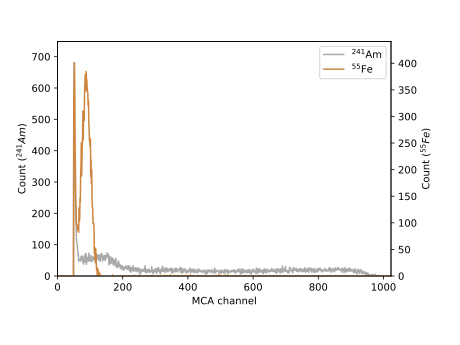
\includegraphics[width=\textwidth]{fig/python/spectra_custom_preamp}
\caption{Measured spectra with the custom pre-amplifier}
\label{fig:pre_amp_testing}
\end{figure}

\begin{figure}[ht!]
\centering
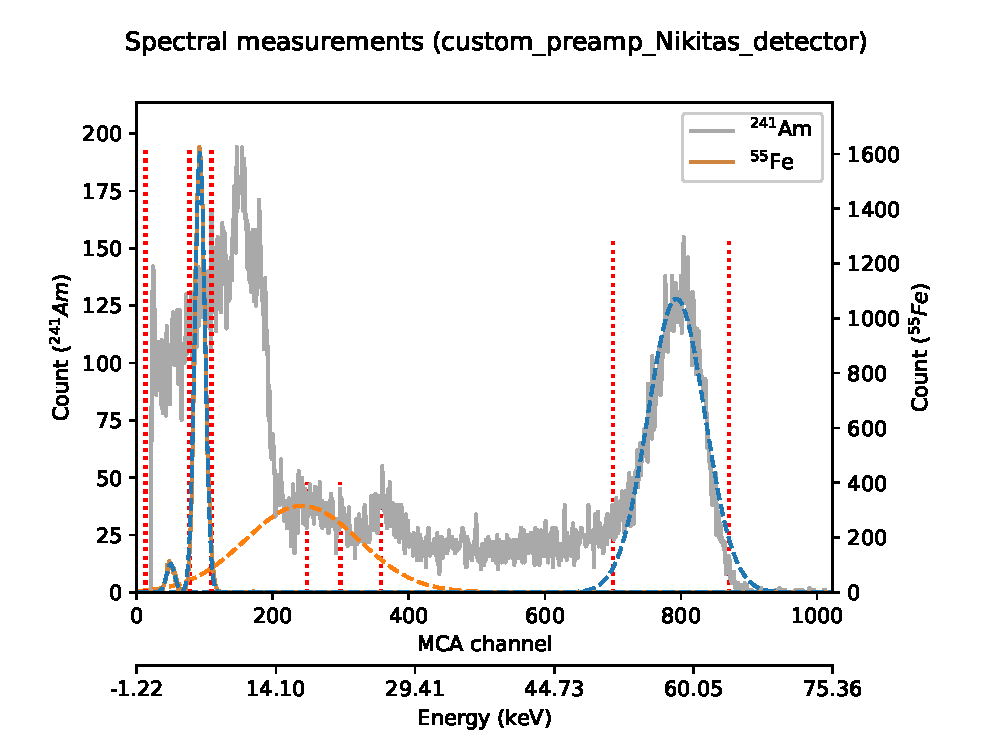
\includegraphics[width=\textwidth]{fig/python/spectra_custom_preamp_Nikitas_detector}
\caption{Measured spectra with the custom pre-amplifier and a coursemate's detector}
\label{fig:pre_amp_testing_nikita}
\end{figure}



\clearpage
\section{Measurement data}
This appendix contains additional information on the measurement results.
The numerical values of the size measurements discussed in section \ref{assembly} are provided in table \ref{table:sizes}.

\begin{table}[ht!]
\centering
\caption{Size measurements
}
\begin{tabular}{l|l|l}
Measurement & $\mu$ & $\sigma$ \\
% \begin{tabularx}{\textwidth}{l|lllll|l|l}
% Measurement & \multicolumn{5}{l}{Data} & $\mu$ & $\sigma$ \\
\hline
Can outer diameter (mm)
% & 66.01 & 65.74 & 65.81 & 65.70 & 65.89
& 65.83 & 0.11 \\
Can top end inner diameter (mm)
% & 47.50 & 47.78 & 47.58 & 47.76 & 47.47
& 47.62 & 0.13 \\
Can top end outer diameter (mm)
% & 53.84 & 53.88 & 53.98 & 53.89 & 53.82
& 53.88 & 0.06 \\
Can bottom end inner diameter (mm)
% & 45.51 & 44.93 & 45.40 & 45.43 & 45.47
& 45.35 & 0.21 \\
Can thickness (\textmu m, from top section)
% & 240 & 250 & 240 & 250 & 280
& 252 & 15 \\
Can thickness (\textmu m, from cut can)
% & 102 & 103 & 102 & 100 & 102
& 101.8 & 1.0 \\
Long brass tube length (mm)
% & 29.25 & 29.26 & 29.27 & 29.27 & 29.25
& 29.26 & 0.09 \\
Short brass tube length (mm)
% & 10.05 & 9.98 & 9.99 & 9.99 & 10.04
& 10.02 & 0.03 \\
Brass tube diameter (µm)
% & 992 & 990 & 991 & 990 & 987
& 990.0 & 1.7 \\
Brass tube + connector length from acryl (mm)
% & 27.30 & 27.15 & 27.32 & 27.59 & 27.23
& 27.32 & 0.15 \\
Anode wire diameter (\textmu m)
& 49.0 & 2.0 \\
% \end{tabularx}
\end{tabular}
\label{table:sizes}
\end{table}


\clearpage
\section{Measurement notes}

This appendix contains copies of some of the original measurement note files.
The rest are formatted as large spreadsheets and could not therefore be included here.
However, all of the files are available in the GitHub repository.
\cite{repo}

\subsection{Environmental measurements}
\lstinputlisting{../analysis/data/notes/environment.txt}

\subsection{Gas leakage test}
\lstinputlisting{../analysis/data/notes/gas_leakage_test.txt}

\subsection{Size measurements}
{
% \UseRawInputEncoding
\lstinputlisting{../analysis/data/notes/size_measurements.txt}
}


\end{appendices}


\clearpage
\printbibliography


\end{document}